%%%%%%%%%%%%%%%%%%%%%%%%%%%%%%%%%%%%%%%%%%%%%%%%%%%%%%%%%%%%
%%% Based on LaPreprint: PREPRINT TEMPLATE
%%% Source: https://github.com/roaldarbol/LaPreprint/tree/b32e34b797298ed151e979e0871b36ec06108110
%%%%%%%%%%%%%%%%%%%%%%%%%%%%%%%%%%%%%%%%%%%%%%%%%%%%%%%%%%%%


% Declare document class
\documentclass[9pt,biorxiv,lineno,onehalfspacing]{lapreprint}
% Choose between "biorxiv", "medrxiv", "arxiv" and "chemrxiv". Otherwise defaults "Preprint".
% Choose between "blue" and "red" colour scheme. Defaults to "blue".
% Use the "onehalfspacing" option for 1.5 line spacing.
% Use the "doublespacing" option for 2.0 line spacing.
% Use the "lineno" option for line numbers.
% Use the "endfloat" option to place floats after the bibliography.

% Import packages
\usepackage{pdflscape}  % For putting pages in landscape mode
\usepackage{rotating}   % For rotating specific elements
\usepackage{textgreek}  % Greek symbols
\usepackage{gensymb}    % Symbols
\usepackage[misc]{ifsym} % For the \Letter symbol
\usepackage{orcidlink}  % For the \orcidlink
\usepackage{listings}   % For inserting code chunks
\lstset{
basicstyle=\small\ttfamily,
columns=flexible,
breaklines=true
}
\usepackage{colortbl}   % For Knitr table colouring
\usepackage{tabularx}   % For making Knitr tables compatible
\usepackage{longtable}  % For multi-page tables
\usepackage[labelformat=simple]{subcaption}
\usepackage{multirow}
\usepackage{snotez}     % For sidenote environments. enotez for endnotes
\usepackage{csquotes}   % For language-based quote rules (helps BiBLaTeX)

%\usepackage[table,xcdraw]{xcolor}
\usepackage[utf8]{inputenc}
%\usepackage[all]{hypcap}
\usepackage{microtype} %makes text formatting slightly more readable
\usepackage{libertine} %uses open source font
\usepackage{svg}
\usepackage{authblk}
\usepackage[labelfont=bf]{caption}
\usepackage{adjustbox}
\usepackage{pgffor}

% for annotated equations
\usepackage{annotate-equations}
\usepackage{amsmath}
%\usepackage{amssymb}
\usepackage{mathtools}
\usepackage{tikz}
\usetikzlibrary{backgrounds}
\usetikzlibrary{arrows,shapes}
\usetikzlibrary{tikzmark} % for \tikzmarknode
\usetikzlibrary{calc} % for computing the midpoint between two nodes, e.g. at ($(p1.north)!0.5!(p2.north)$) 
\newcommand{\highlight}[2]{\colorbox{#1!17}{$#2$}}
\newcommand{\highlightdark}[2]{\colorbox{#1!47}{$#2$}}
\newcommand\ttiny{\fontsize{4}{5}\selectfont}
\newcommand\tttiny{\fontsize{2}{3}\selectfont}

\hypersetup{
  colorlinks   = true, %Colours links instead of ugly boxes
  urlcolor     = blue, %Colour for external hyperlinks
  linkcolor    = gray, %Colour of internal links
  citecolor    = gray  %Colour of citations
}

%%%%%%%%%%%%%%%%%%%%%%%%%%%%%%%%%%%%%%%%%%%%%%%%%%%%%%%%%%%%
%%% BIBLIOGRAPHY
%%%%%%%%%%%%%%%%%%%%%%%%%%%%%%%%%%%%%%%%%%%%%%%%%%%%%%%%%%%%
\usepackage[			% use biblatex for bibliography
	backend=biber,      % use biber or bibtex backend
    style=numeric-comp,   % choose style
	natbib=true,		% allow natbib commands
	hyperref=true,	    % activate hyperref support
	alldates=year,      % only show year (not month)
    uniquename=false,   % don't add firstnames when citing multiple sources by the same author
    maxbibnames=12,     % maximum number of author names to list in bibliography before 'et al' is used instead
    sorting=none,       % sort by order of appearance
]{biblatex}

\AtEveryBibitem{
    \clearfield{urlyear}
    \clearfield{urlmonth}
    \clearlist{language}
    \clearfield{url}
    \clearfield{note}
   % \clearfield{issn}
}

% Update to your bibliography file
\addbibresource{bib.bib}
\addbibresource{Dec2023-Converted.bib}


%%%%%%%%%%%%%%%%%%%%%%%%%%%%%%%%%%%%%%%%%%%%%%%%%%%%%%%%%%%%
%%% ARTICLE SETUP
%%%%%%%%%%%%%%%%%%%%%%%%%%%%%%%%%%%%%%%%%%%%%%%%%%%%%%%%%%%%

% Paper title
\title{The origin of color categories}
\shorttitle{The origin of color categories}

\author[ \orcidlink{0000-0002-4579-003X} 1 \Letter]{Daniel J. Garside}
\author[ \orcidlink{0000-0002-2532-9780} 1,2,*]{Audrey L.Y. Chang}
\author[ \orcidlink{0000-0003-1570-9576} 1,*]{Hannah M. Selwyn}
\author[ \orcidlink{0000-0001-7715-9253} 1,3 \Letter]{Bevil R. Conway}

% Affiliations
\affil[1]{Laboratory of Sensorimotor Research, National Eye Institute, National Institutes of Health}
\affil[2]{present address: Vilcek Institute of Graduate Biomedical Sciences, New York University}
\affil[3]{National Institute of Mental Health}
\affil[*]{these authors contributed equally}

% Other metadata. Feel free to add your own
\metadata[]{\Letter\hspace{.5ex} For correspondence}{ \href{mailto:danny.garside@nih.gov}{danny.garside@nih.gov} or \href{mailto:bevil@nih.gov}{bevil@nih.gov}}

%\metadata[\authfn{1}\authfn{2}\authfn{3}]{}{Here's a few symbols to denote contribution specifics, e.g. authors who contributed equally to the work.} %!!!!!!!!!!!!!
%\metadata[]{Present address}{49 Convent Drive, Bethesda, MD-20892-4435, USA} 
% \metadata[]{Data availability}{Data availability statement. 
% Preprocessed data could be available e.g. on \href{https://zenodo.org/}{Zenodo}.} %!!!!!!!!!!!!!!!!
\metadata[]{Data availability statement}{All data and code are available on \href{https://github.com/NEI-LSR/MacaqueColorCategories}{github.com/NEI-LSR/MacaqueColorCategories}}
\metadata[]{Code availability statement}{All data and code are available on \href{https://github.com/NEI-LSR/MacaqueColorCategories}{github.com/NEI-LSR/MacaqueColorCategories}}
\metadata[]{Funding}{This research was supported by the Intramural Research Program of the NIH, National Eye Institute.}
\metadata[]{Competing interests}{The authors declare no competing interests.} 

% Surname of the lead author(s) for the running footer
\leadauthor{Garside}

%%%%%%%%%%%%%%%%%%%%%%%%%%%%%%%%%%%%%%%%%%%%%%%%%%%%%%%%%%%%
%%% ARTICLE START
%%%%%%%%%%%%%%%%%%%%%%%%%%%%%%%%%%%%%%%%%%%%%%%%%%%%%%%%%%%%


\begin{document}
\maketitle
\begin{refsection}

\begin{abstract}

To what extent does concept formation require language? Here we exploit color to address this question and ask if macaque monkeys have color concepts evident as categories. Macaques have similar cone photoreceptors and central visual circuits to humans, yet they lack language. Whether Old World monkeys such as macaques have consensus color categories is unresolved, but if they do, then language cannot be required. If macaques do not have color categories, then color categories in humans are unlikely to derive from innate properties of visual encoding and likely to depend on cognitive abilities such as language that differ between monkeys and humans. We tested macaques by adapting a match-to-sample paradigm used in humans to uncover color categories from errors in matches, and analyzed the data using computational simulations that assess the possibility of unrecognized distortions in the perceptual uniformity of color space. The results confirm that humans have consensus cognitive color categories and show that macaques do not. One animal showed evidence for a private color category, demonstrating that monkeys have the capacity to form color categories even if they do not form consensus color categories. Taken together, the results imply that consensus color categories in humans, for which there is ample evidence, must depend upon language or other cognitive abilities.

\end{abstract}

\begin{figure}
    \begin{fullwidth}
    \centering
    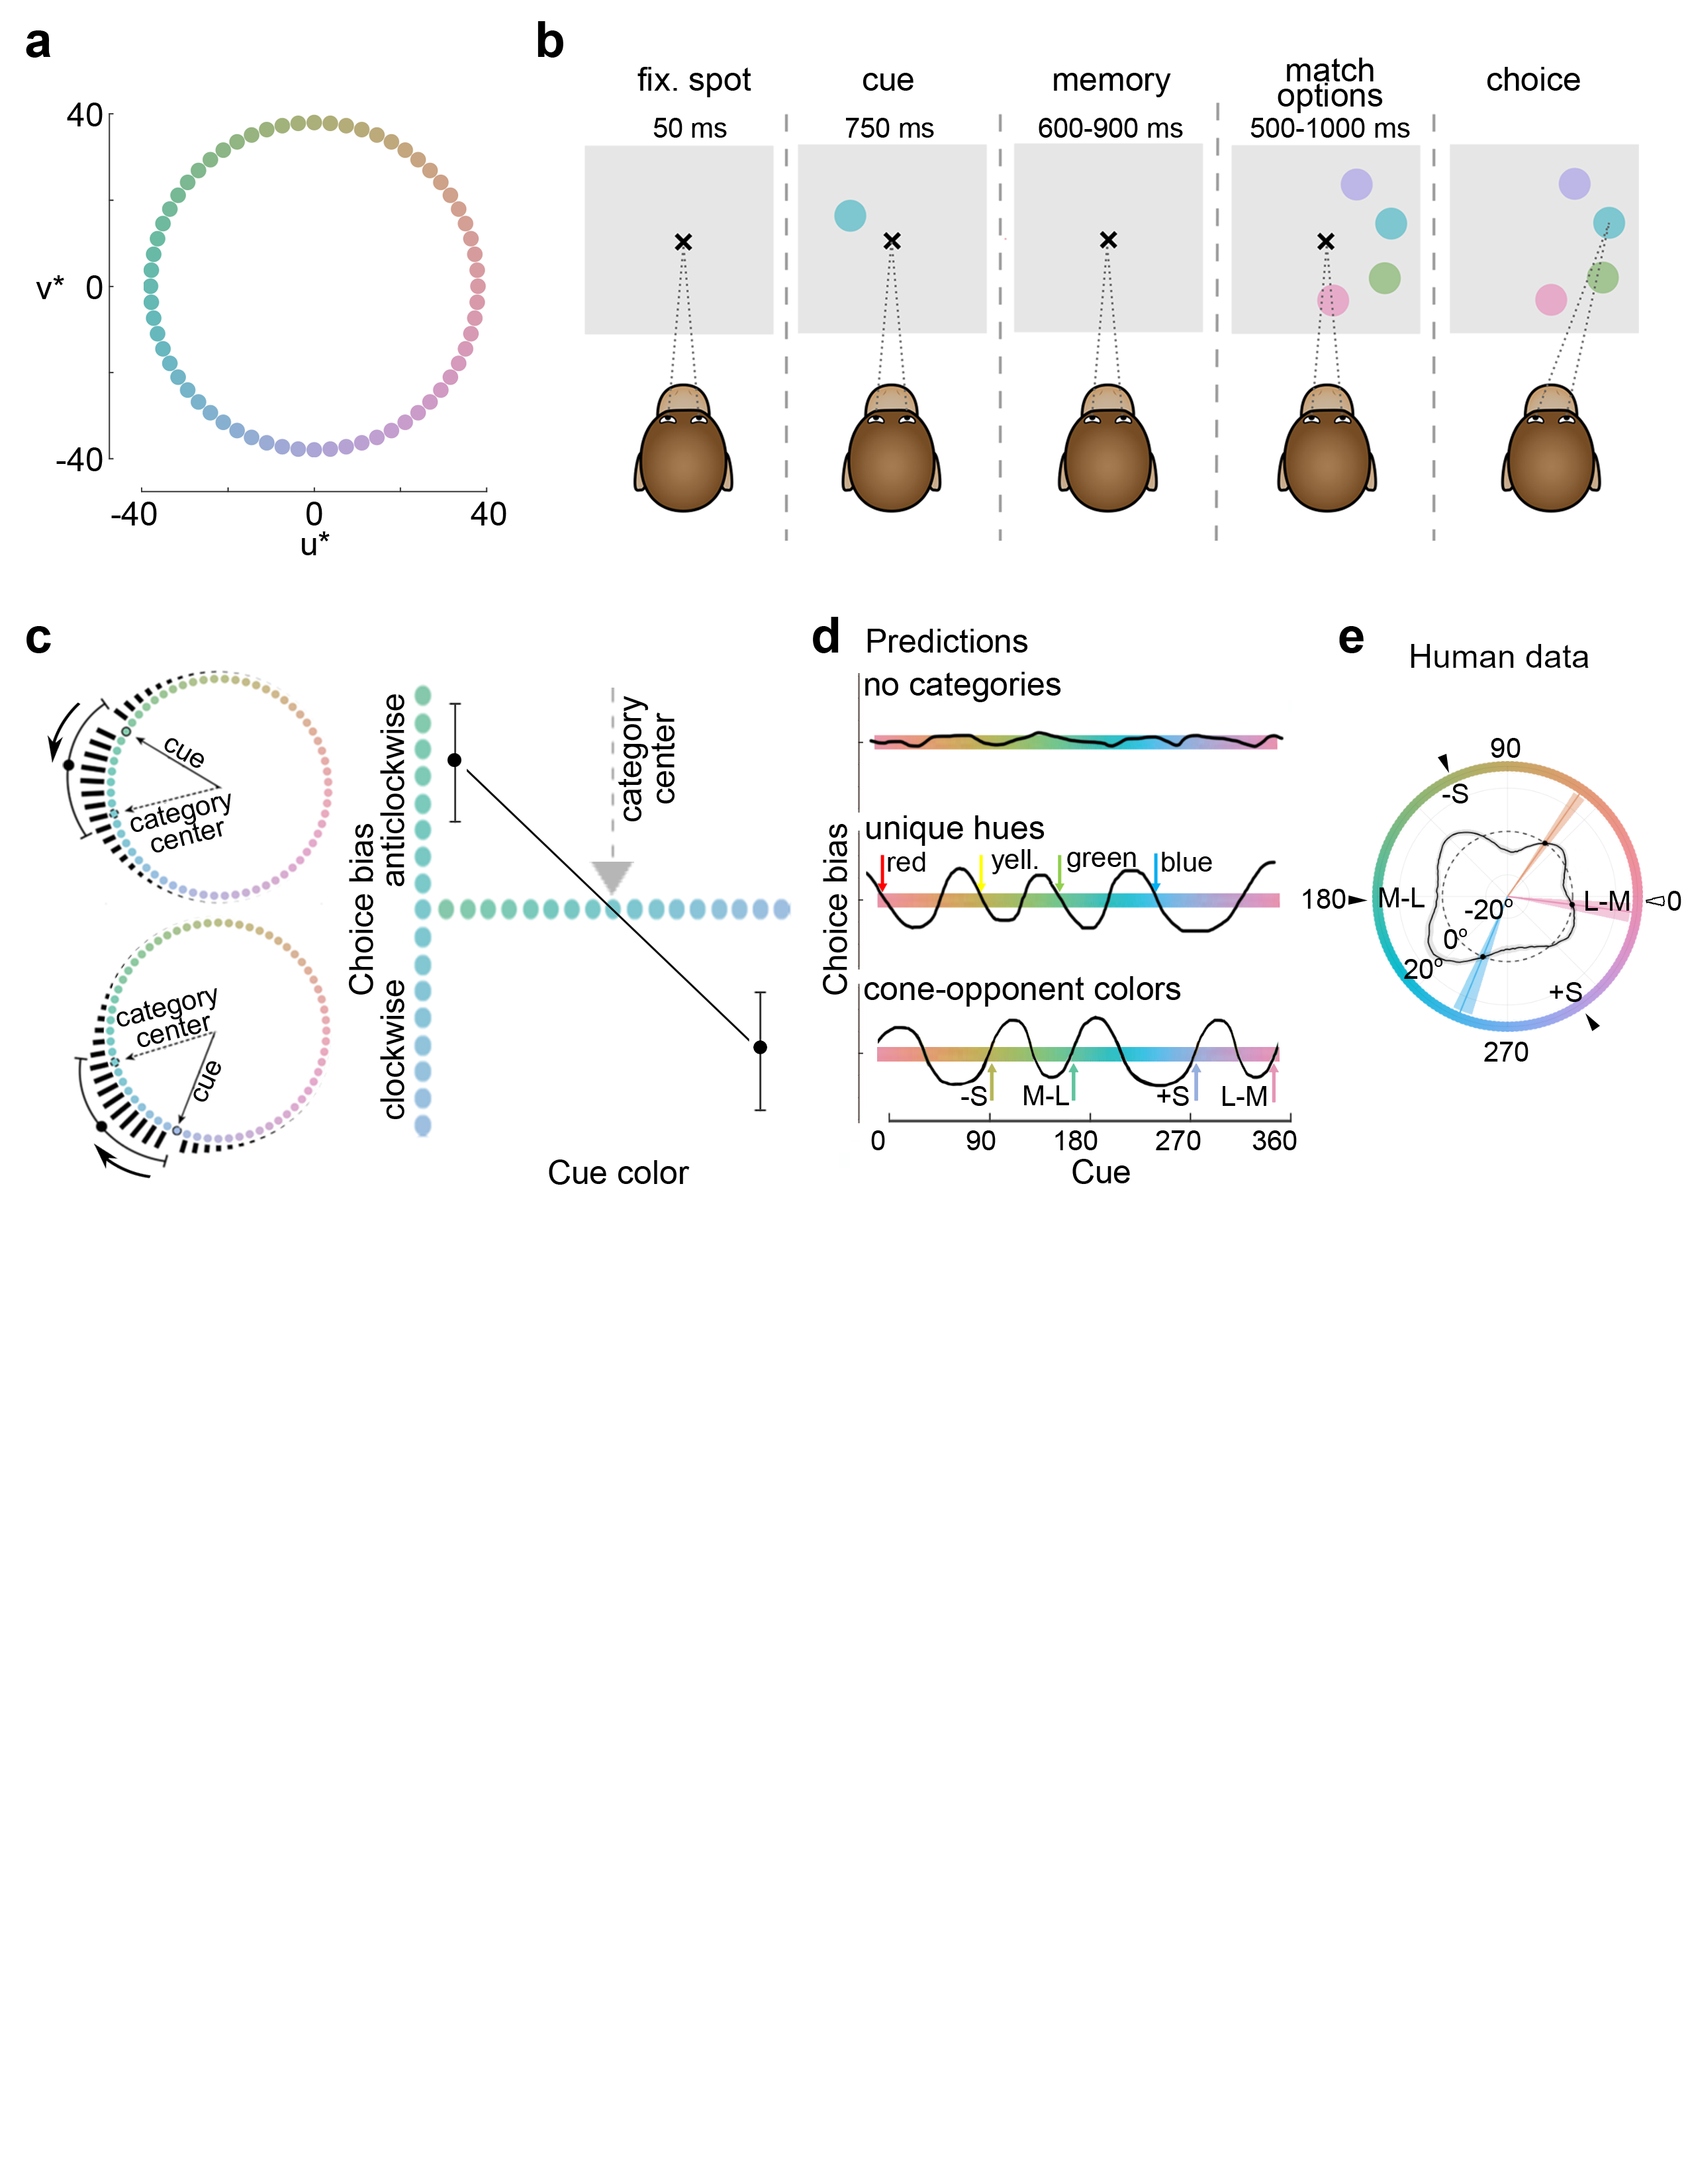
\includegraphics[width=\textwidth+4cm,trim={0 12.5cm 0 0},clip]{Outputs/Paper/Figures/flat/F1_ParadigmPredictions_9.png}
    \caption{\textbf{Non-verbal paradigm to recover color categories in non-human primates.}
    \textbf{a}, Sixty-four Colors defined in CIELUV color space. 
	\textbf{b}, Animals were trained to initiate a trial by fixating a small cross on a computer monitor and to maintain fixation throughout the trial until the fixation cross disappeared, which was their instruction to make a choice; trials in which the animals broke fixation were aborted. 
	A 3\degree{} diameter cue was presented within the central 2.5 – 6\degree{}, followed by a variable memory delay (600-900ms) and the presentation of four choice options. 
	To mitigate impulsive choices, the choice options were shown for a variable amount of time (500-1000 ms) during which the animals needed to maintain fixation to avoid aborting the trial. 
    After the fixation cross disappeared, the animals were free to make their selection. 
	\textbf{c}, Predicted distribution of choices for two cues if a color category exists at the specified location in the color space (dashed arrow). 
	The average of the distribution of choices will be biased counterclockwise from the cue if the cue is displaced clockwise to the category center (top) and biased clockwise from the cue if the cue is displaced counterclockwise to the category center (bottom). 
    This pattern of results would be captured as the zero-crossing of the negative slope in a plot of the choice bias versus cue color (right). 
	\textbf{d}, Predicted pattern of results for three hypotheses: no categories (top); categories defined by attractors to the four common basic color categories (middle); and categories defined by repellors to the cone-opponent retinal encoding mechanisms (bottom). 
	\textbf{e}, Data obtained in prior work on a related task in human subjects showing evidence of four color categories. 
    Though there are only 3 zero-crossings in the dataset presented here (that of \citet{bae_why_2015}) the data shows a periodic structure with 4 cycles, with a fourth attractor point suggested at roughly 180\degree{} (green). 
    See SI Figure 2 for two additional data sets in human subjects including the prior work of \citet{panichello_error-correcting_2019} and new data using the present task; all infer the existence of four consensus color categories. 
    The negative slopes demarking category centers are recovered by tracing the line in a counterclockwise direction, at points where the trace crosses the dashed circle marking zero choice bias. 
    For reference, arrowheads show the colors that would isolate the retinal cone-opponent encoding mechanisms (L-M, M-L, +S, -S; where L, M, S are the three cone types).}
    \label{fig:ParadigmAnalysisPredictions}
    \end{fullwidth}
\end{figure}

Color categories are identified by color terms, of which the Basic Color Terms are considered prominent \citep{berlin_basic_1969}.
One hypothesis is that a subset of these terms---red, green, blue, yellow---express universal concepts \citep{heider_universals_1972,regier_focal_2005}
that are endowed by hard-wired neural mechanisms present at birth \citep{bornstein_categories_1976,lindsey_universality_2006}. 
This idea, put forth 150 years ago \citep{hering_zur_1875}, predicts common patterns in color naming across cultures \citep{baronchelli_modeling_2010,lindsey_hunter-gatherer_2015,abbott_focal_2016}
and finds some neurophysiological support in human infants \citep{clifford_electrophysiological_2009,yang_cortical_2016}. 
Behavioral work in infants also provides evidence for a biological origin of color categories \citep{franklin_new_2004,ozturk_language_2013} and suggests that color categories may build on an innate scaffolding defined by retinal cone-opponent mechanisms \citep{skelton_biological_2017}. 
The infants in all these experiments were at least several months old, by which stage they would have had substantial cultural exposure, so the evidence that they express color categories cannot be conclusively ascribed to an innate origin. 
Another hypothesis is that color categories emerge in development, instructed by language and culture \citep{davidoff_colour_1999,roberson_color_2005}, possibly involving an interplay of innate and developmental factors \citep{webster_variations_2002,kay_language_2006,franklin_lateralization_2008,regier_language_2009,paramei_online_2018}. 
Support for this hypothesis is provided by the variability in color-naming patterns across languages \citep{davidoff_colour_1999,webster_variations_2002,roberson_color_2005,kay_language_2006,gibson_color_2017, paramei_online_2018}. 
Current consensus is that at least some aspect of color category behavior is acquired through experience. But the extent to which color categories are innate remains unresolved \citep{davidoff_nature_2009,RN18696,RN18699}(see also chapter 6 in \citep{block_border_2023}). Computational theories of color term evolution have been constructed that do not require innate mechanisms (REFS). 

Another approach to studying the origin of color categories could be provided by behavioral experiments in trichromatic non-human primates \citep{sandell_color_1979,carey_where_2009,RN18699,siuda-krzywicka_biological_2019} since they lack language but have almost identical perceptual systems to humans and presumably the same perceptual color space \citep{schnapf_spectral_1987,stoughton_psychophysical_2012,gagin_color-detection_2014, horwitz_what_2015}. Monkeys are widely used as models of human visual cognition because they are thought to have the similar mechanisms of visual memory and visual decision making \citep{panichello_error-correcting_2019,horwitz_what_2015}. The few studies on this topic have come to different conclusions: one found color categories in macaque monkeys consistent with categories in human adults \citep{sandell_color_1979}, implying that color categories do not depend on language and may be innate.
This study inadvertently made comparisons substantially easier for cross-category than within-category trials, undermining its conclusion \citep{davidoff_cross-species_2010}. 
A later study tested for the existence of color categories across a limited range of colors and found a blue-green boundary in humans but not baboons \citep{fagot_cross-species_2006,RN18699}. The lack of color categories in the baboons might reflect the limited survey of color space (blues and greens are categorized with high variability in all languages, including English \citep{gibson_color_2017}). A third study, designed to investigate visual working memory, uncovered a different pattern of results in the two animals tested \citep{panichello_error-correcting_2019}, raising the possibility that the two animals had private color categories. 

\paragraph{Measuring color categories in macaque monkeys}

Addressing the question of color categories in monkeys requires overcoming several challenges. 
First, how can color categories be measured non-verbally, without teaching the animals the categories or reinforcing idiosyncratic biases \citep{essock_color_1977,matsuno_color_2004}? 
Second, how should the color stimuli be chosen \citep{siuda-krzywicka_biological_2019}?
For example, choosing colors according to their wavelength equivalent 
\citep{sandell_color_1979} is not appropriate 
\citep{davidoff_cross-species_2010}.
Third, how can data across the full circle of hues be obtained so as to avoid missing categories \citep{fagot_cross-species_2006}? 
A match-to-sample paradigm, using colors defined in a perceptually uniform color space \citep{stockman_colorimetry_2010} (Figure 1a), provides a potential solution to these challenges, because, as demonstrated for human subjects, color categories introduce biases in the distribution of matches \citep{bae_why_2015}. 
So color categories could be inferred from any observed biases across the space of colors without requiring participants to understand or produce linguistic labels.  

This works in human participants who can follow instructions but introduces complications in monkeys because it is not clear how to reward the animals. 
Rewarding them for picking a color in the vicinity of the color of the cue could reinforce idiosyncratic biases, which is not a problem for addressing certain questions \citep{panichello_error-correcting_2019} but would be a problem for recovering consensus categories; moreover, the response metric (an eye movement or pointed finger) could confound the perceptual decision with motor noise. 
To overcome these complications, we adapted the paradigm as an alternative-forced-choice task in which a direct match to the cue was available in every trial and the monkeys were only rewarded for making the direct match with an eye movement (Figure 1b). 
The precision of the eye tracker (\textasciitilde0.3\degree{} of visual angle) was considerably finer than the size of the choice options (3\degree{} diameter). 
One consequence of the adapted paradigm is that it requires a much larger number of trials to satisfactorily assess the similarity relationships of each color to every other color. 
Four animals performed the task, completing a total of 209456 trials over 232 sessions (SI Figure 1).

Following the logic of \citet{bae_why_2015} - if a monkey has a color category, the category center will be an attractor in the color space. 
An attractor would be captured by a zero-crossing of negative slope in a plot of choice bias (Figure 1c). 
Repellors, meanwhile, would be captured by zero-crossings of positive slope. 
The approach is data-driven, so it will recover whatever categories exist; nonetheless, before collecting the data we considered three possibilities. 
First, that the monkeys would show no color categories, predicted by the work sampling a limited range of colors in baboons \citep{davidoff_cross-species_2010} (Figure 1d, top). 
Second, that the monkeys would show four color categories, predicted by attractor points defined by the four putatively universal basic color terms (Figure 1d, middle). 
Third, that the monkeys would show four color categories, but predicted by data in human infants corresponding to repellor points defined by physiological cone-opponent mechanisms not basic color terms \citep{skelton_biological_2017} (Figure 1d, bottom).

For reference, Figure 1e shows the results of a prior study in human adults \citep{bae_why_2015}, where the results are compatible with the second and third possibilities outlined above. 
Note that the authors of the original study show that the data is best explained by a model with four attractors, even though there are only three zero-crossings. 
The four recovered color categories do not perfectly line up with the four common basic terms; instead they correspond to pink, orange, green, blue.
The discrepancy may arise because of limitations imposed by ensuring equal saturation and luminance among the colors (the resulting set of stimuli has neither a good red nor a good yellow) (see \citep{bae_why_2015}). 
The four categories could also be seen as corresponding to the physiological cone-opponent mechanisms - each pole (denoted by labeled arrowheads) seems to roughly correspond to a repellor point (positive zero-crossing), with the exception of the L-M pole.
The recovery of four categories, at roughly matching locations, has been replicated in English speakers \citep{panichello_error-correcting_2019} across multiple versions of the task, including by us in new data collected using the discrete-matching version used presently (SI Figure 2). 

\begin{figure}
    \begin{fullwidth}
    \centering
    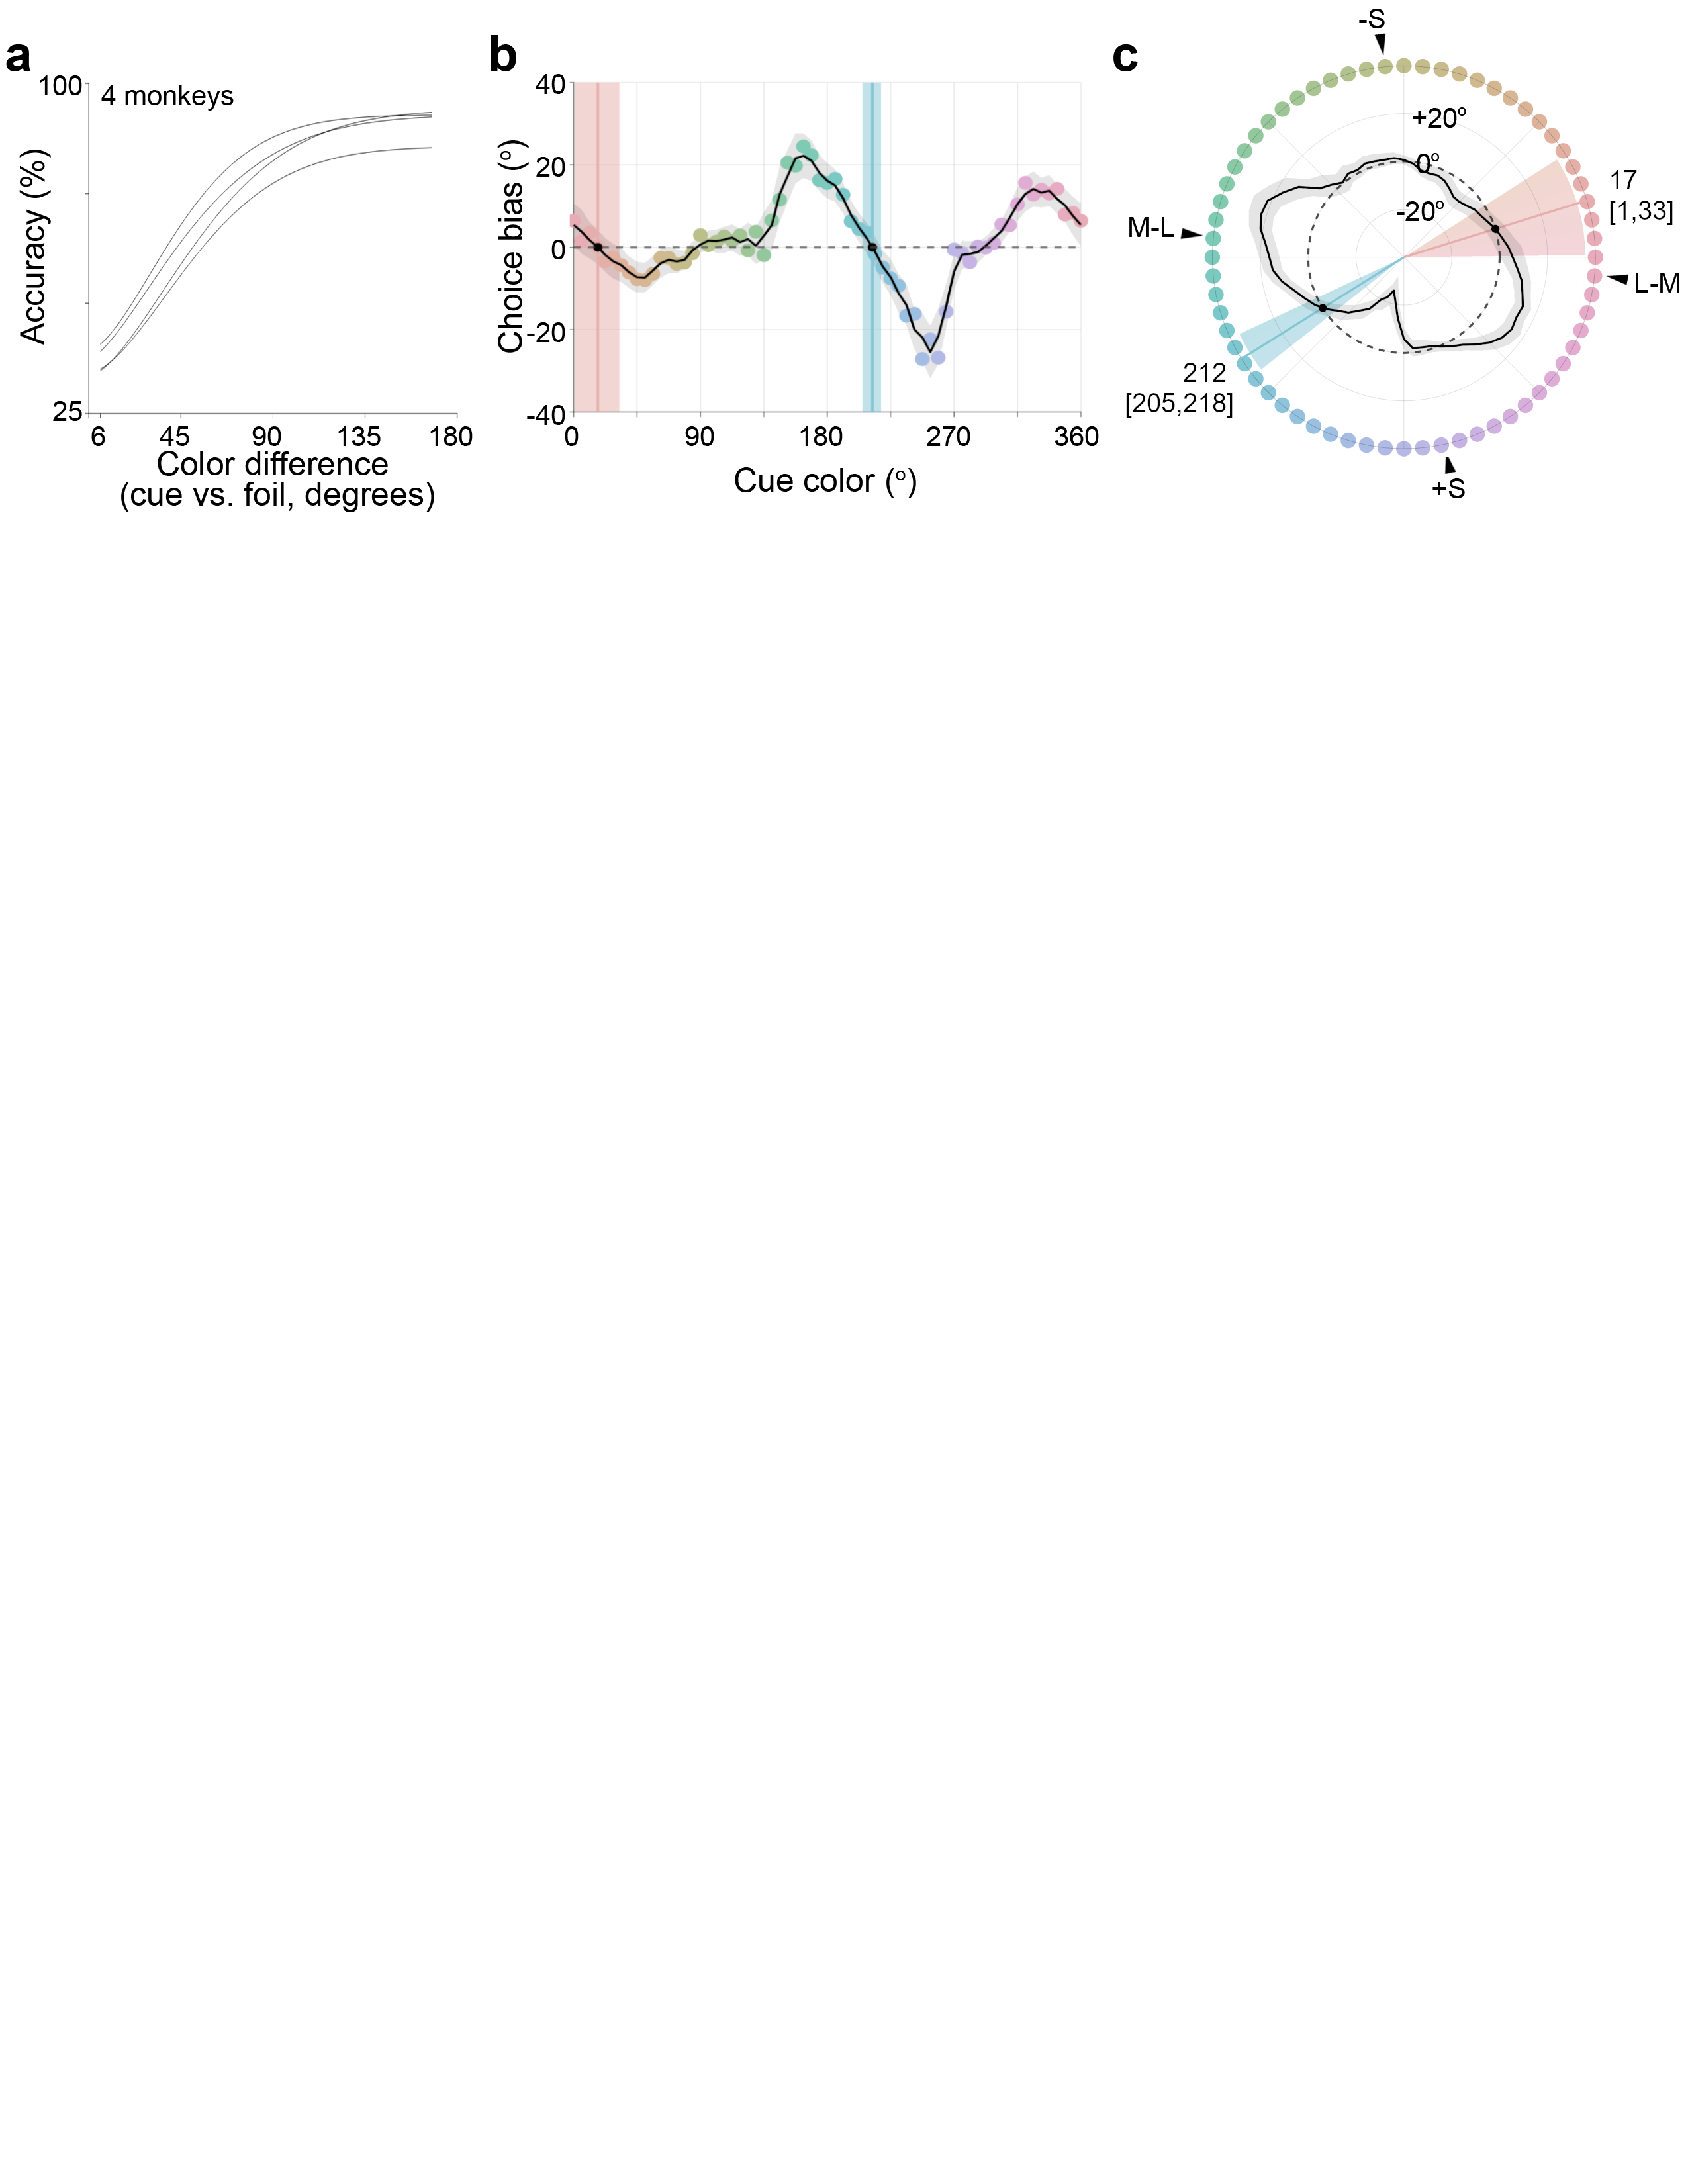
\includegraphics[width=\textwidth+4cm,trim={0 21cm 0 0},clip]{Outputs/Paper/Figures/flat/F2_CombinedMMResults_6.png}
    \caption{\textbf{Macaque monkeys appear to show two consensus color categories when the data are analyzed with a mixture model that computes the average distribution of the choices for each cue.}
	\textbf{a}, Psychometric functions for the four animals showing the accuracy of the matches as a function of the difference in hue angle between the cue and the foil that is closest in color to the cue. 
	The easiest trials were defined as those where the foil color nearest to the cue color were almost on the opposite side of the color circle. See SI Figure 2 for 95\% CI. 
	\textbf{b}, Mixture model results averaged across the four animals. 
    The data were subsampled so that the same number of completed trials for each animal (24526) were included in the analysis, corresponding to [9475, 9694, 10665, 9783] incorrect trials respectively for PO, CA, BU, MO. 
    Error shading shows 95 \%CI. 
	The data recover two significant negative-slope zero-crossings (black dots), corresponding to two color categories. 
	\textbf{c}, Polar plot of the results in (b) with the zero-crossings of the negative slope (following the trace counterclockwise) again indicated by black dots. 
    The angle of the two inferred color categories [95 \% C.I.] are 17 [1, 33] (a peach color) and 212 [205, 218] (a teal color). }
    \label{fig:AvResults}
    \end{fullwidth}
\end{figure}

The four animals performed well on the task, achieving lapse rates of 7.0\%, 7.1\%, 5.8\%, 14.3\% respectively on the easiest trials (Figure 2a; the plots of individual animals showing 95\% CI are provided in SI Figure 1). 
The results averaged across the four animals, analyzed using the mixture model as used previously to analyze data collected in humans \citep{bae_why_2015,zhang_discrete_2008} (see Methods), provided clear evidence of choice biases (Figure 2, SI Figure 3). 
But the apparent color categories shared among all animals inferred using this analysis do not support any of the predictions: the animals appeared to show two consensus color categories, not four as in humans. 
To the extent that the macaque is an accurate model of a non-linguistic human, these results show that the four color categories manifest in humans are not innate. 
The centers of the two apparent consensus color categories recovered in the monkeys were at 17\degree{} (a peach color) and 212\degree{} (a teal color). 
All four animals showed evidence of these two color categories (SI Figure 4).

\paragraph{Two possible explanations for choice biases in macaque monkeys}

\begin{figure}
    \begin{fullwidth}
    \centering
    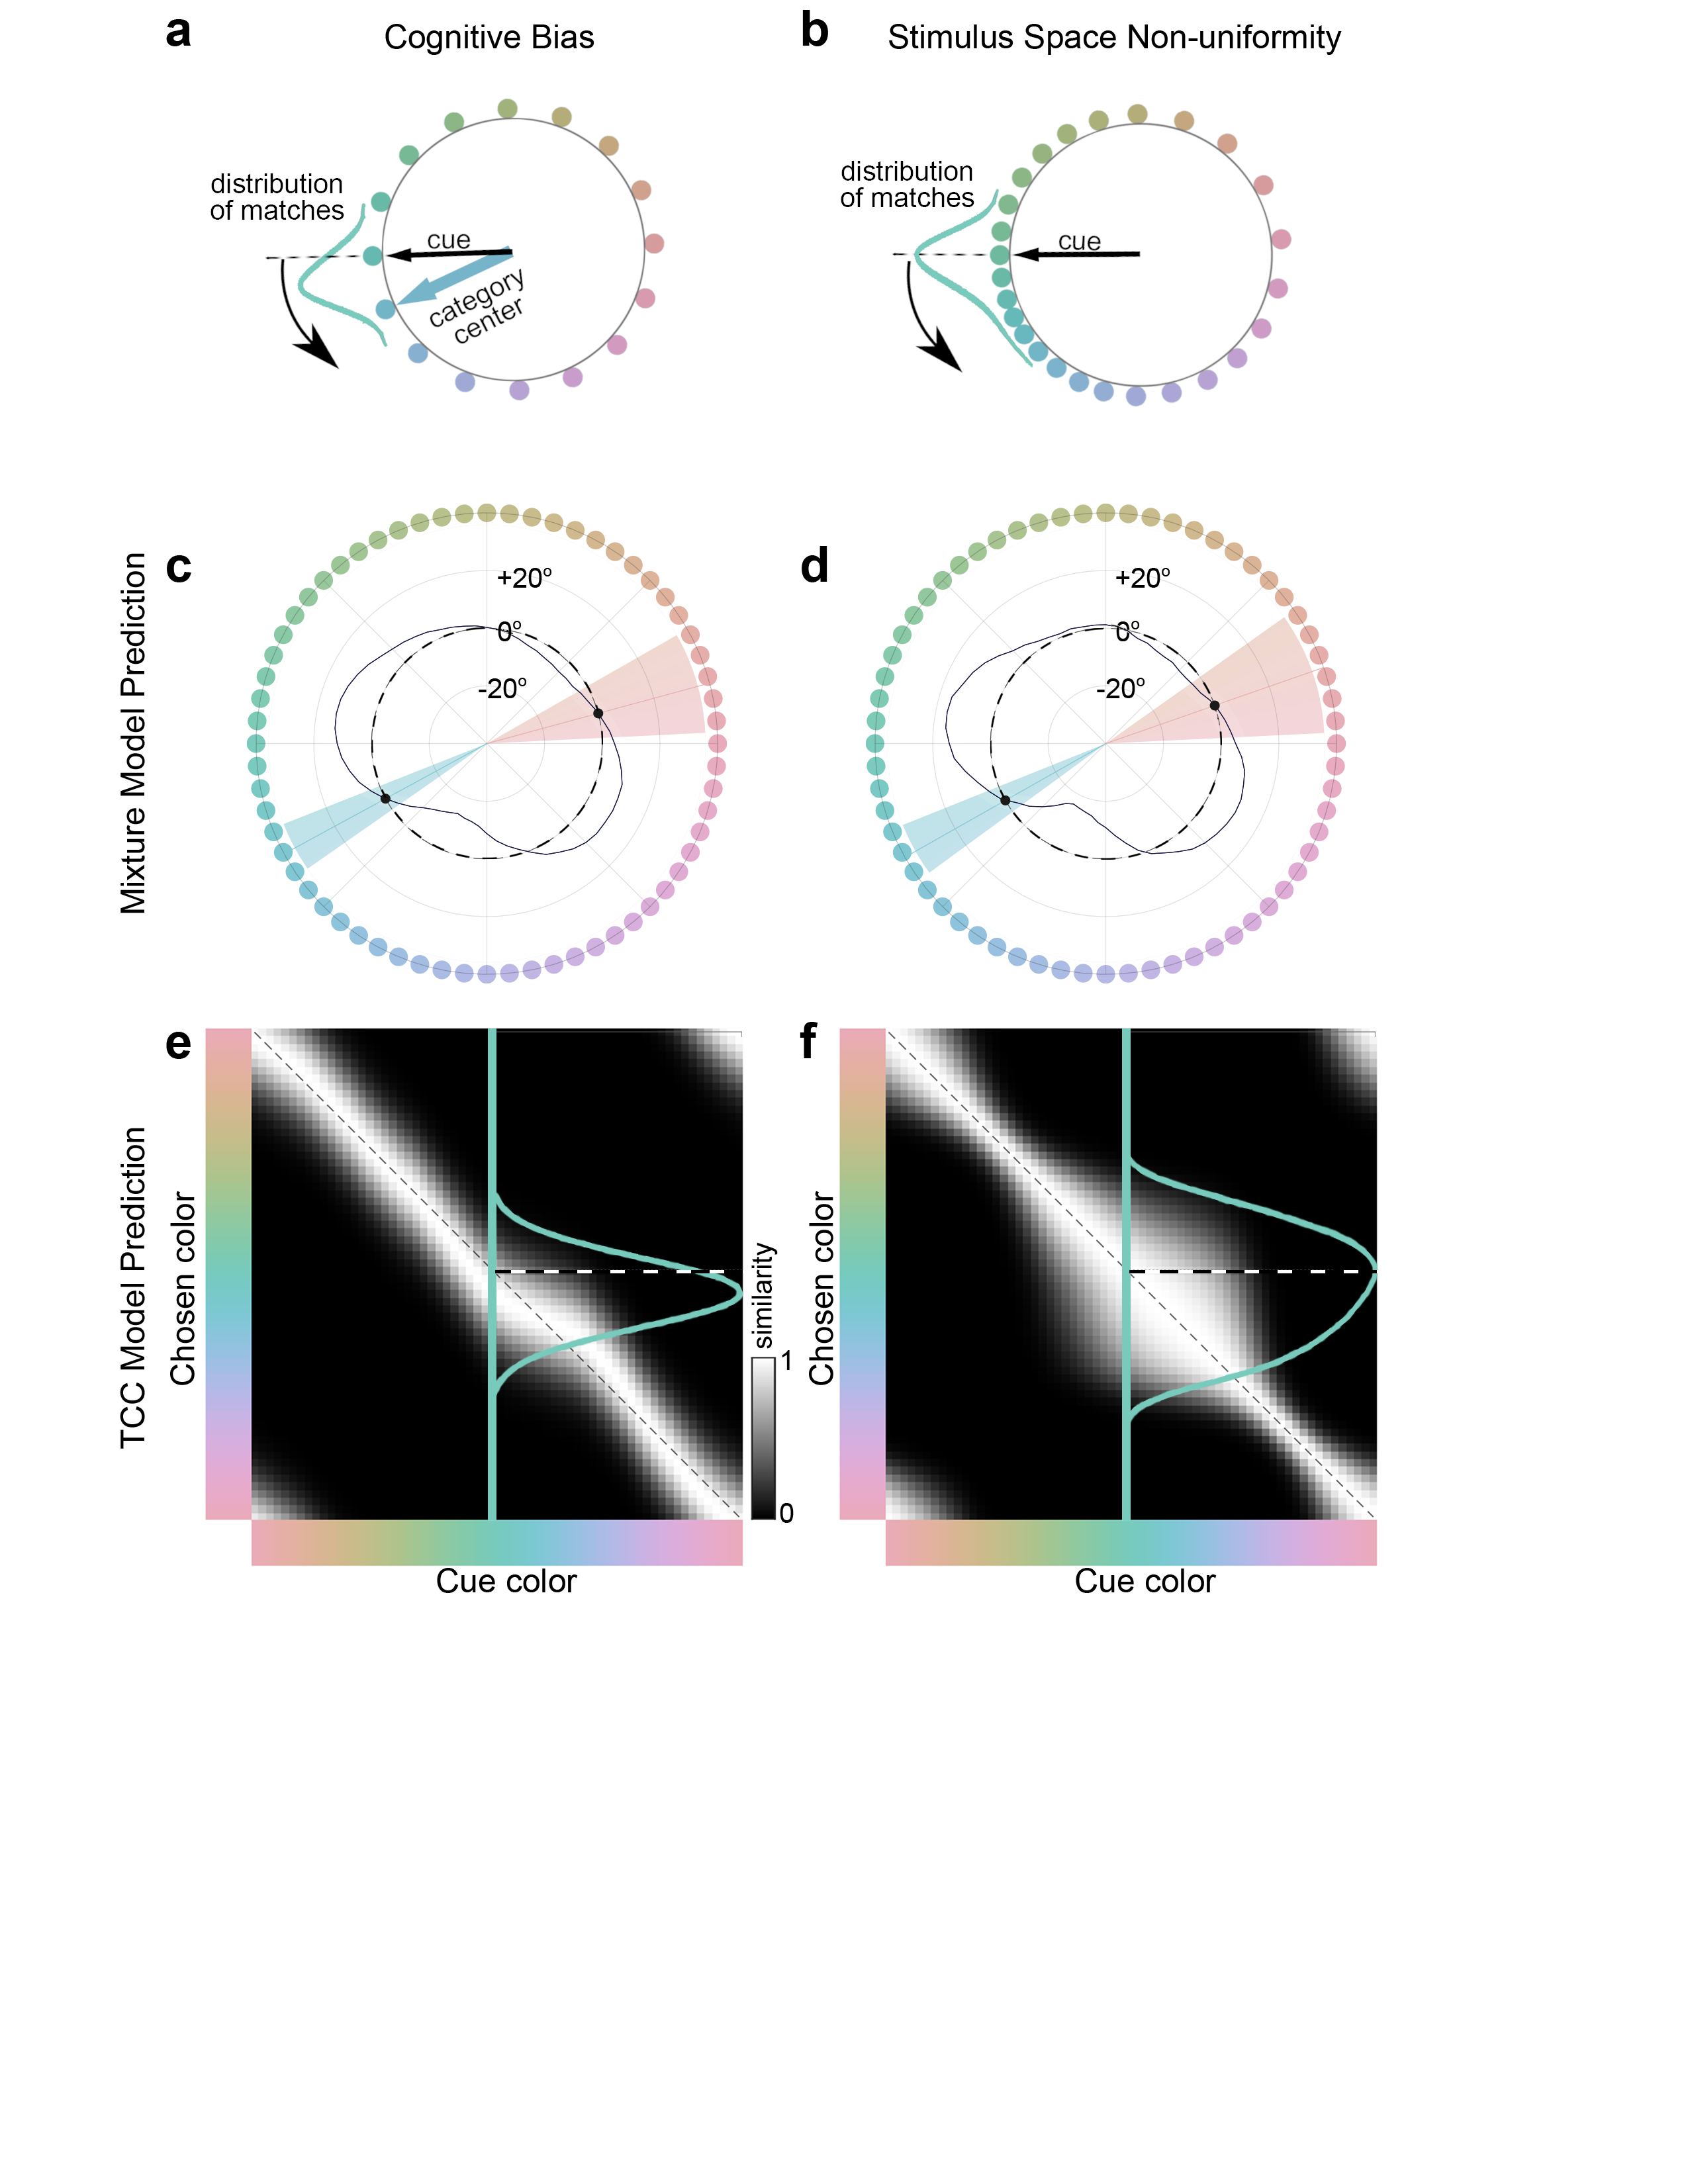
\includegraphics[width=\textwidth,trim={0 7cm 0 0},clip]{Outputs/Paper/Figures/flat/F3_TCCModel_7.png}
    \caption{\textbf{Computational simulations showing that color choice biases recovered by mixture model \citep{zhang_discrete_2008, bae_why_2015} could be explained by a non-uniformity in the stimulus space, without invoking cognitive mechanisms.} 
    \textbf{a}, Color matches made by an agent with a cognitive color category, using a paradigm with stimuli that uniformly sample a truly uniform perceptual color space (gray circle). 
    The distribution of matches has a peak biased towards the category center.
    \textbf{b}, Color matches made by an agent lacking a cognitive color category, with stimuli that non-uniformly sample an underlying uniform color space (gray circle). 
    The distribution of matches is biased towards the densely sampled region of the space because there are more choice options. 
    The average of the distribution of matches is similarly biased counterclockwise to the cue in both a and b, although the similarity functions differ in shape. \textbf{c}, Mixture-model analysis of a simulated data set with a cognitive bias; \href{https://github.com/NEI-LSR/MacaqueColorCategories/blob/main/Outputs/Paper/Figures/working/F3_TCCModel/Code/F3ace_TCCModel_OffsetGaussian.m}{Code for F3c} \textbf{d}, Mixture-model analysis of a simulated data set with a stimulus space non-uniformity. 
    \href{https://github.com/NEI-LSR/MacaqueColorCategories/blob/main/Outputs/Paper/Figures/working/F3_TCCModel/Code/F3bdf_TCCModel_StimulusSpaceNonUnifomity.m}{Code for F3d}
    \textbf{e}, Similarity matrix for the simulated data analyzed in c; axes are CIELUV color space. 
    Each column shows the similarity function for the corresponding cue on the x axis. 
    The trace shows the similarity function for the cue in a. 
    Note that the shape of the similarity function is symmetric like the distribution of matches. \href{https://github.com/NEI-LSR/MacaqueColorCategories/blob/main/Outputs/Paper/Figures/working/F3_TCCModel/Code/F3ace_TCCModel_OffsetGaussian.m}{Code for F3e} \textbf{f}, Similarity matrix for the simulated data analyzed in panel d; other details as in e. 
    \href{https://github.com/NEI-LSR/MacaqueColorCategories/blob/main/Outputs/Paper/Figures/working/F3_TCCModel/Code/F3bdf_TCCModel_StimulusSpaceNonUnifomity.m}{Code for F3f}. The shape of the similarity function is different in e and f, yet both have the same mean bias relative to the cue. 
    The similarity function in f and the distribution of matches in b are both asymmetric but differ in shape because the color spaces are different in b and f.}
    \label{fig:TCCDemo}
    \end{fullwidth}
\end{figure}

The colors we used were sampled in CIELUV - a colorspace defined by the International Commission on Illumination with the goal of being perceptually uniform. 
But it has long been recognized that there may be non-uniformities in all color spaces, including this one \citep{stockman_colorimetry_2010}; some authors have argued that perceptual uniformity may be task-dependent or simply unattainable \citep{judd_ideal_1970,bujack_non-riemannian_2022}. 
One might even suppose that if language influences color perception, as stipulated by the cultural-relativity hypothesis \citep{roberson_color_2005}, then all color spaces generated by human observers could be shaped by language. 
Could the macaque consensus color categories be attributed not to a true cognitive category (Figure 3a) but to unrecognized distortions in the presumed uniform space of colors (Figure 3b)? 
Both explanations could introduce biases in the distribution of matches (the mean for the distribution of matches will be biased away from the cue, curved arrows Figure 3a and 3b).

The difference in the two explanations can be understood by considering the relationship between two neighboring colors in the color space. 
For the cognitive-bias account, there is an asymmetry between neighbors if there is a category center nearby. 
The color further from the category center will be more likely mistaken for the color closer to the category center than the other way around. 
In the non-uniform color space explanation however, there is no asymmetry in mismatches between neighboring colors, but if a neighbor on one side is more confusable than a neighbor on the other side then a bias will be introduced. 
Both explanations lead to a distribution of matches that is shifted away from the cue. 
We refer to the distributions of matches for a given cue, plotted in CIELUV, as the similarity function for that cue, and the family of similarity functions for all cues as the similarity matrix.
A cognitive bias would yield similarity functions of constant width for all cues around the color circle, but the function peaks would deviate from their respective cues depending on the proximity of the category center. 
A stimulus space non-uniformity, meanwhile, would yield an asymmetric similarity function which peaks at the cue but varies in width and shape depending on sampling density of the true underlying uniform color space, with regions that are relatively densely sampled having broader distributions.

To illustrate that the behavioral data could be explained by either a cognitive-bias account or a stimulus-space non-uniformity, we generated two sets of simulated data.
One data set was generated with a simulation that used a uniform space and a bias arising from two cognitive categories, and the other data set was generated with a simulation that used non-uniform sampling of an underlying uniform color space and no cognitive categories. 
The data sets from both simulations gave rise to the same pattern of results when analyzed with a mixture model \citep{zhang_discrete_2008, bae_why_2015} (Figure 3c and 3d). 
These simulated data sets were specified to match the pattern of biases recovered in our behavioral results (compare the simulated results in Figures 3c,d, with Figure 2c). 

To decide which of these explanations best accounts for the macaque behavioral data, we developed computational models of each mechanism and analyzed the data with an extension of the Target Confusability Competition (TCC) model \citep{schurgin_psychophysical_2020} (see Methods). 
The standard implementation of the TCC model assumes the same similarity function for each color. 
The version developed presently allows the shape and/or location of the similarity function to vary per color (we refer to the modified TCC model as TCC-v, for "vary"). 
Let's consider three versions of the TCC-v model. 
First, the simplest ("null") model has the same similarity function for each color, centered on the target color (this is conceptually equivalent to the original TCC model). 
This model has two free parameters ($\sigma$, $d'$) which control the width of the Gaussian similarity function and the amount of noise present in the system respectively.
Second, the "cognitive bias" version of the model specifies similarity functions for each color with peaks that can deviate from the target color but in which all similarity functions for the set of colors have the same symmetric (Gaussian) shape (Figure 3a). 
In addition to $\sigma$ and $d'$, this model has an additional set of 64 parameters which control the offset of the peak of the similarity function - one for each color.
The result is a similarity matrix that has a band of constant height along the inverse diagonal but deviates to one side near color-category locations in the color space (Figure 3e). 
Third, the "stimulus-space non-uniformity" version of the model has a fixed similarity function across colors, but the perceptual distances between colors can differ, which results in a similarity function which is distorted when it is plotted as a function of stimulus index.
In addition to $\sigma$ and $d'$, this model has an additional set of 64 parameters which control the relative angular perceptual distance between each successive color.
This results in a similarity matrix that is symmetric about the inverse diagonal, but which bulges out away from the diagonal at locations in the color space that are oversampled (Figure 3f). 
The stimulus-space non-uniformity model and the cognitive-bias model have the same number of parameters. 

To recap, the similarity matrix in 3e is constructed using the same data as the polar plot in 3c, and the similarity matrix in 3f is constructed using the same data as the polar plot in 3d. 
Panels c,d use the standard mixture-model approach which does not allow an asymmetry in the shapes of the similarity functions. 
Panels e,f, use the TCC-v approach, which permits the similarity functions to vary. 
The results of these computational simulations show that different underlying mechanisms could explain the appearance of choice biases in color-matching tasks when evaluated with the standard mixture model.

In an additional version of the TCC-v model ("free-similarity") we treat every cell in the similarity matrix as an independent model parameter (Figure 4a, 4b; the data for both panels are the same, centered on one or the other of the putative category centers recovered in the mixture model; free similarity matrices for the individual animals are shown in SI Figure 5). 
The free-similarity matrix makes no assumptions about the underlying functions that determine the similarity between any pair of stimuli (in contrast to the prior models which assume a Gaussian with specific manipulations). 
Such a model is hugely flexible, which would allow for non-hypothesized mechanisms to be surfaced (for example: a "favorite color" bias would appear as a vertical line).
It also gives us a very intuitive and visual way to ask: is the average free similarity matrix better explained by the stimulus space non-uniformity model or the cognitive bias model? 
In other words, do the panels in Figure 4a and 4b show mirror symmetry with bulges about the diagonal (like Figure 3f) or asymmetry about the diagonal without bulges (like Figure 3e)? 

\begin{figure}
    \begin{fullwidth}
    \centering
    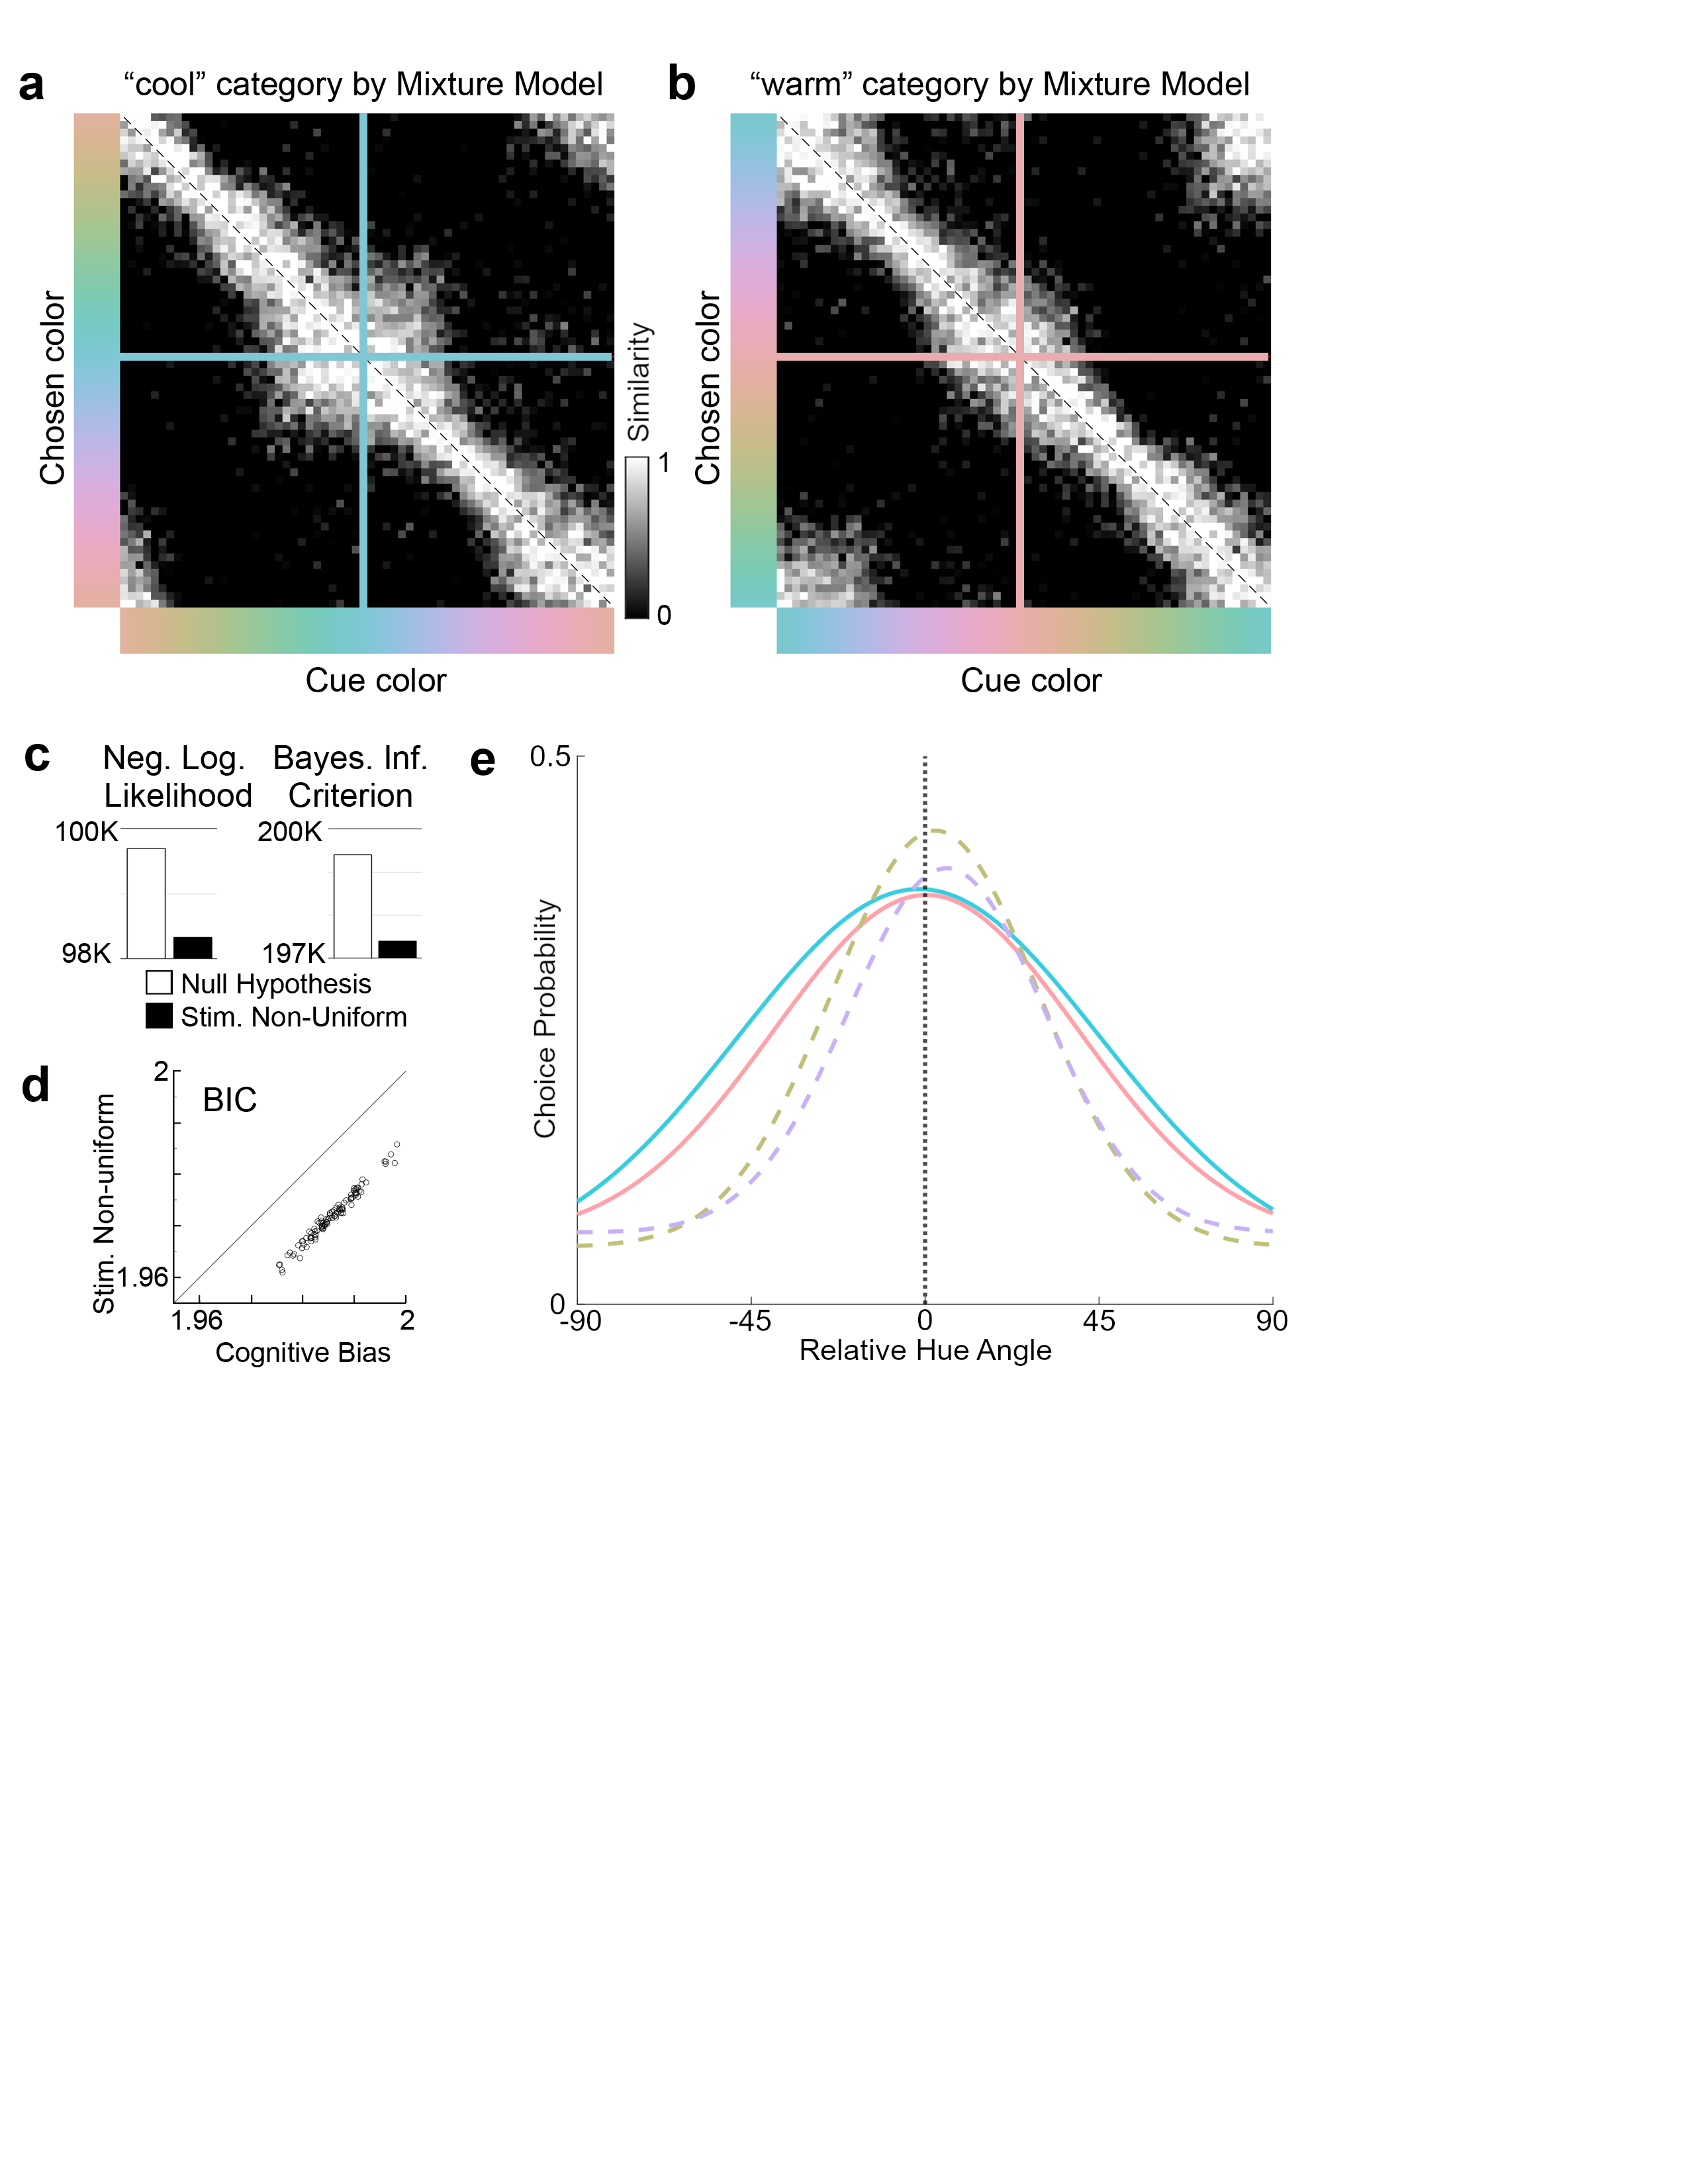
\includegraphics[width=\textwidth,trim={0 10cm 4cm 0},clip]{Outputs/Paper/Figures/flat/F4_TCCResults_4.png}
    \caption{\textbf{Similarity matrices for behavioral data averaged across four monkeys}
    \textbf{a}, Data centered on the teal-colored category recovered in the mixture model.  
	\textbf{b}, Data centered on the peach-colored category recovered in the mixture model. The pattern of results in a, b is better predicted by stimulus space non-uniformity (Figure 3f) than cognitive bias (Figure 3e). 
	\textbf{c}, Negative Log Likelihood (left) and Bayesian Inference Criterion (BIC, right) of the fit of the null model and the stimulus-space non-uniformity model. 
	\textbf{d}, BIC values of the fit provided by the stimulus-space non-uniformity model were always lower than BIC values of the fit for the cognitive bias model for 100 bootstrap repeats of the analysis. 
    For each boostrap repeat, the number of trials for each animal were the same, set by the animal that completed the smallest total number of completed trials, and that number of trials was drawn with replacement from the total number of completed trials for each animal. 
    The stimulus space non-uniformity model and the cognitive bias model have the same number of parameters. 
    \textbf{e}, Gaussian fits (extracted from a mixture model) showing broader gaussians at the two attractor points (solid lines) than at cues 90\degree{} offset (dashed lines).
    } 
    \label{fig:TCCOutput}
    \end{fullwidth}
\end{figure}

By visual inspection, the data are better explained by the stimulus space non-uniformity model, a conclusion affirmed by statistical tests (AIC/BIC for null, cognitive bias, and stimulus-space non-uniformity models respectively are: [199397,198005,196792]/[199416,198616,197402]). 
First, the stimulus space non-uniformity model provides a better fit of the data than the null model (Figure 4c). 
Second, the data are better explained by the stimulus-space non-uniformity model than the cognitive bias model (Figure 4d). 
These results show that the apparent two consensus color categories recovered by the mixture model are explained by a non-uniformity in the underlying color space, and that there is a non-linear mapping of a true perceptually uniform color space and the presumed uniform color space we used. 
These results therefore suggest that macaque monkeys do not have any innate consensus color categories. 
If the macaque is an accurate model of the human, then the results imply that humans do not have innate consensus color categories either. 

\begin{figure}
    \begin{fullwidth}
    \centering
    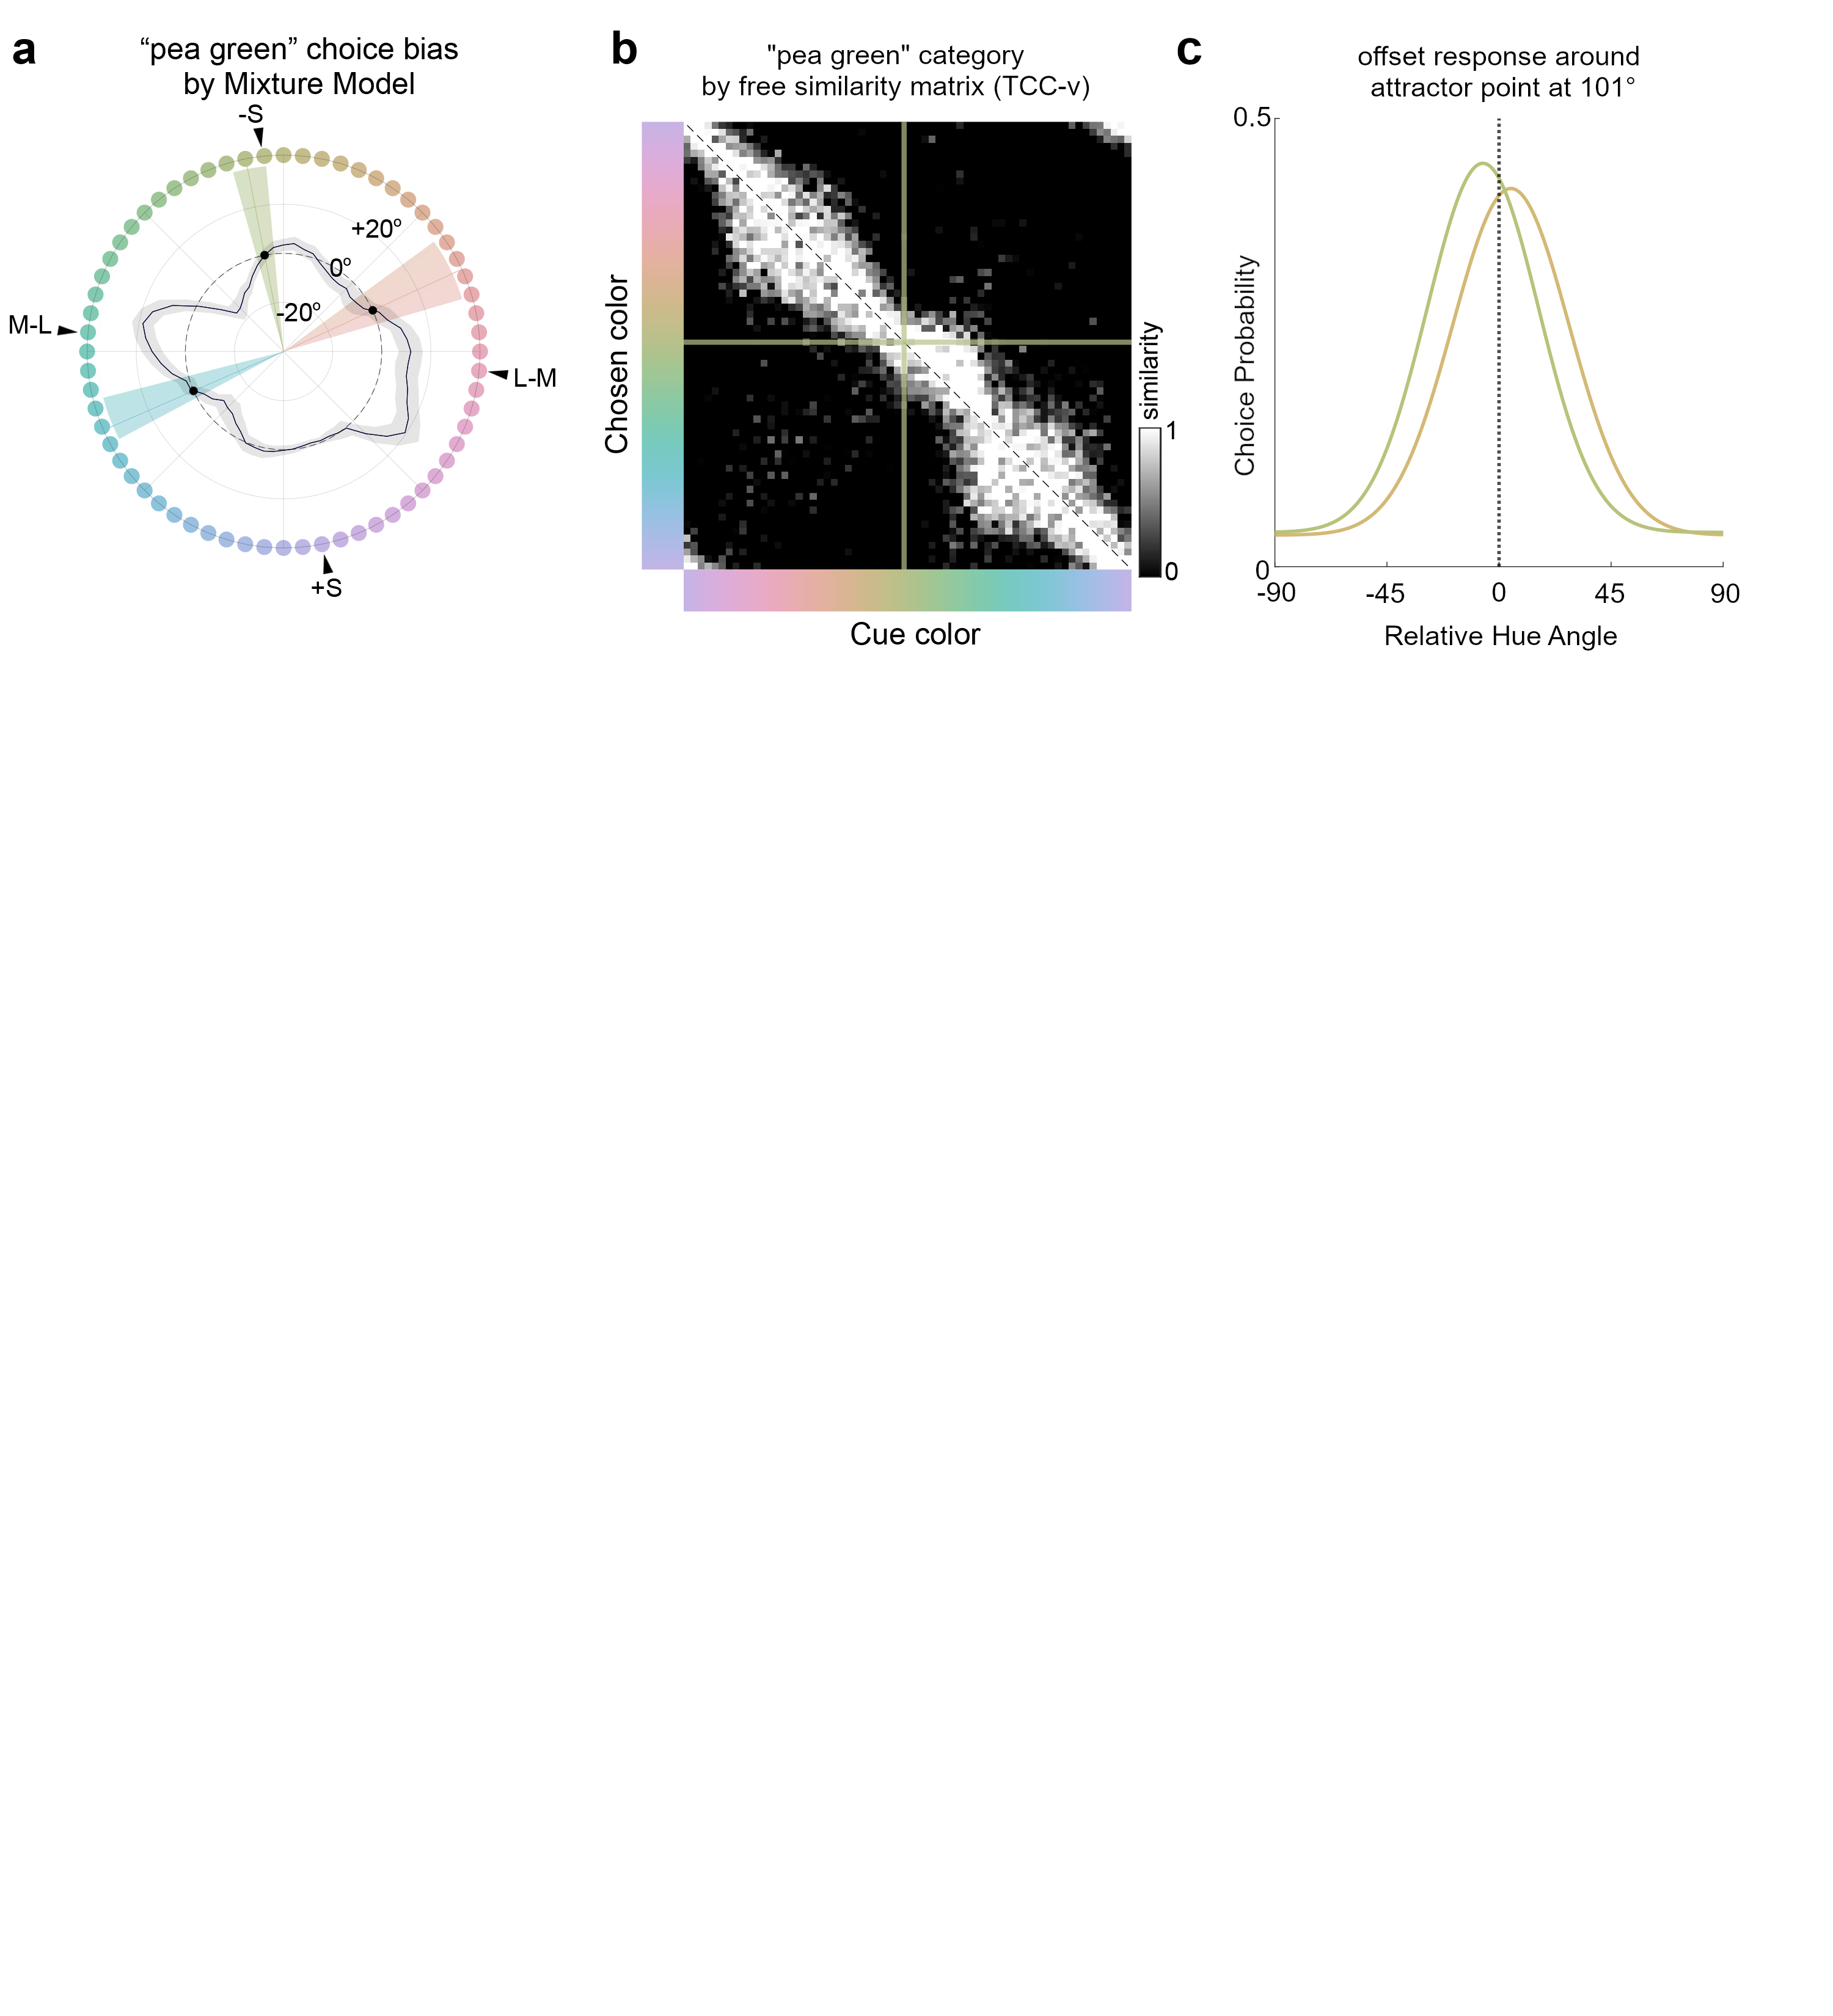
\includegraphics[width=\textwidth+4cm,trim={0 18cm 0 0},clip]{Outputs/Paper/Figures/flat/F5_CastorCogBias_8.png}
    \caption{\textbf {Color-matching data for one monkey (CA) showing evidence for a cognitive color category bias.} 
    \textbf{a}, Mixture-model analysis (same format as Figure 2c). 
	\textbf{b}, Free-similarity matrix (same format as Figure 4a,b) with an asymmetry in the green region indicated by the cross.
    \textbf{c}, Gaussians extracted from the mixture model on either side of the identified attractor point (101\degree{}) showing offsets. 
    Plotted curves are for hue angles 90\degree{} (right, offset to positive values) and 112.5\degree{} (left, offset to negative values).}
    \label{fig:IndiDataCogBias}
    \end{fullwidth}
\end{figure}

The data presented so far are for the four animals combined, which allowed us to assess the existence of consensus color categories. 
But we noted that the individual animals showed some idiosyncratic patterns of results (SI Figure 4, SI Figure 5). 
By mixture-model analysis, one animal showed not only the two consensus choice biases that are explained by stimulus space non-uniformities but also a third bias, for pea green (Figure 5a). 
The free similarity matrix for the data from this animal shows an asymmetry about the diagonal at this location in the color space (Figure 5b), showing that this animal has a cognitive bias---a true color category---for pea-green, in addition to the consensus biases driven by stimulus-space non-uniformities. 
The result in this animal, and trends that the other animals also have idiosyncratic cognitive biases, show that macaque monkeys have the potential to form cognitive color biases, and that the TCC-v model can recover them. 
This is important not simply because it confirms that the ability to form cognitive categories does not require language, as suggested previously \citep{panichello_error-correcting_2019}, but also because it shows that if macaques had consensus color categories, we would have been able to observe them.
AIC/BIC for null, cognitive bias, and stimulus-space non-uniformity models, fit to just this animal's data, are: [97181,96352,95242]/[97200,96962,95853] respectively.
Ideally we would fit a model which allows for the presence of multiple mechanisms simultaneously - while this is already possible in our computational model, there are currently unresolved challenges involved in fitting such a model to real data due to the increased dimensionality. 

\begin{figure}
    \begin{fullwidth}
    \centering
    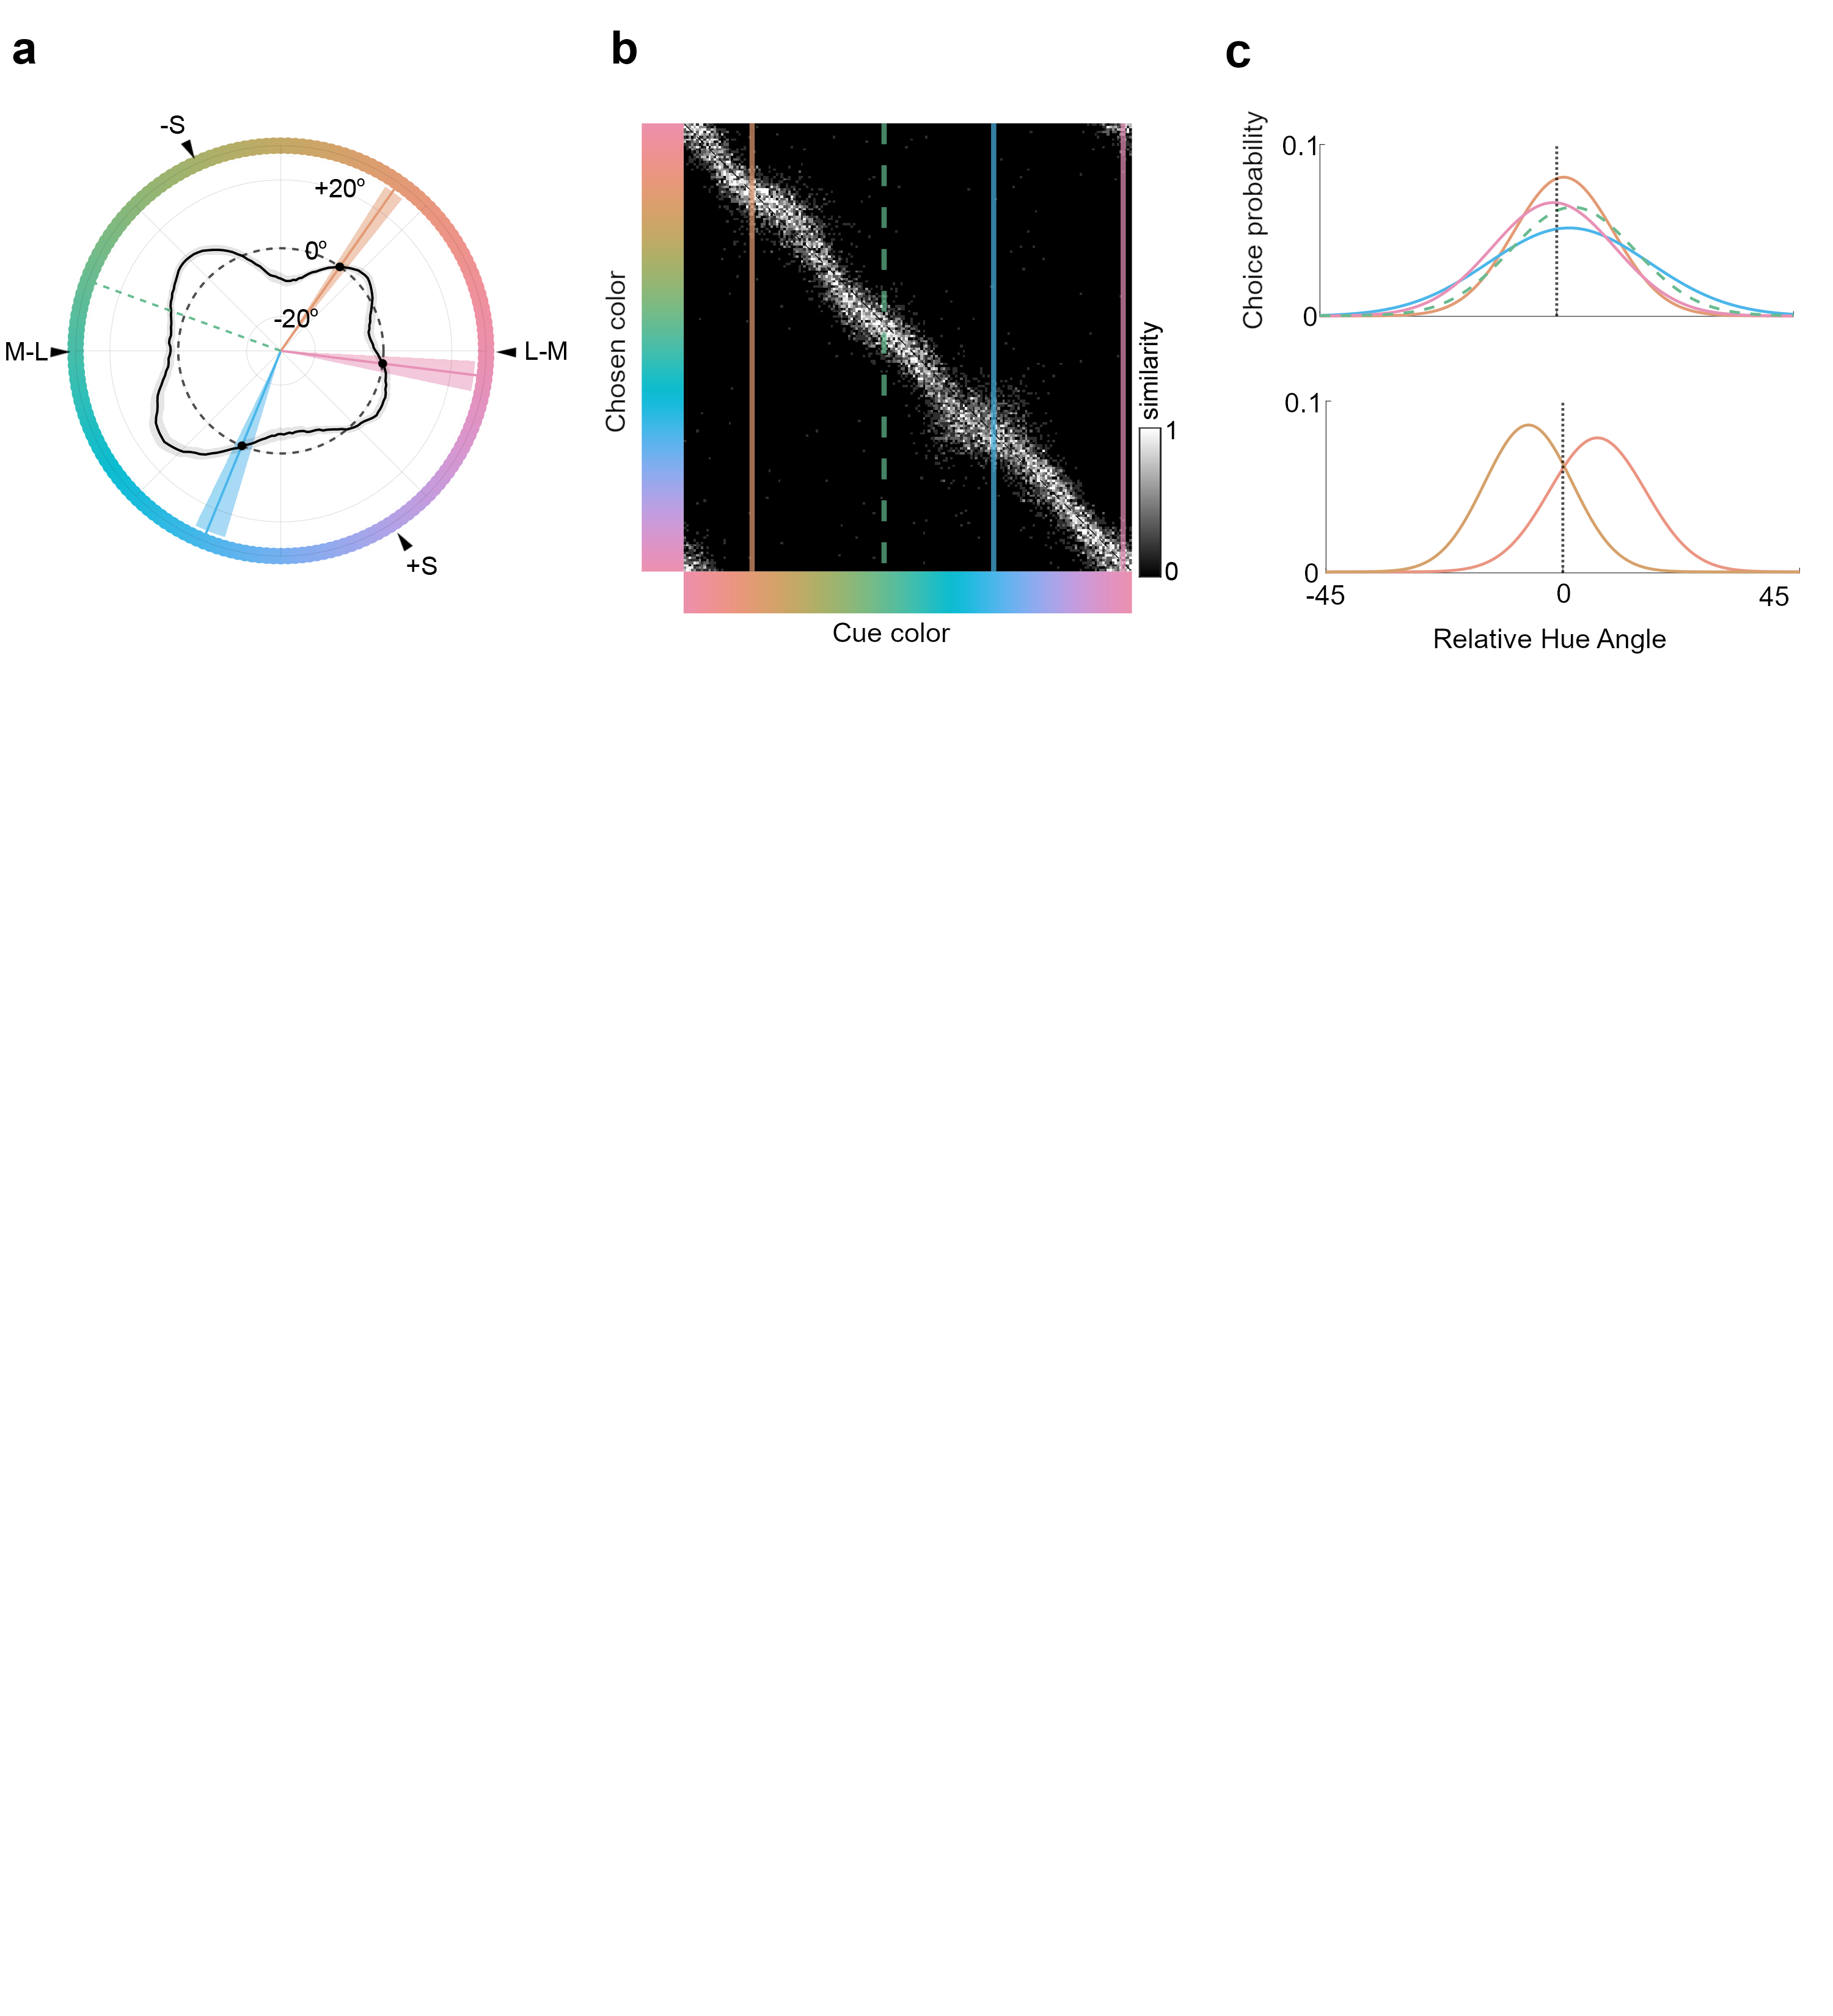
\includegraphics[width=\textwidth+4cm,trim={0 18cm 0 0},clip]{Outputs/Paper/Figures/flat/F5b_HumanMainText_3.png}
    \caption{\textbf {Reanalysis of the data of \citet{bae_why_2015} - what mechanisms underly the observed biases?}
    \textbf{a}, Mixture model analysis of the data of \citet{bae_why_2015} (as in Figure 1e, reproduced for easy reference).
    \textbf{b}, Choice probability matrix of the same data, with the attractor points recovered by the mixture modeling analysis highlighted.
    \textbf{c}, Gaussian fits extracted from the mixture model. 
    Above: Gaussians at the attractor points, showing a range of widths. 
    Below: Gaussians at either side (right, 38\degree{} and left, 70\degree{}) of the orange attractor (54\degree{}), showing offsets towards the attractor.}
    \label{fig:HumanMainText}
    \end{fullwidth}
\end{figure}

\paragraph{Revisiting the human data}

The analysis of the average data collected in monkeys shows no evidence for cognitive biases and strong evidence for stimulus-space non-uniformities, which suggest there are no consensus color categories in monkeys, in contrast with humans. 
But this conclusion depends on (1) the capacity of the task and analysis to recover cognitive biases; and (2) the existence of consensus cognitive color categories in humans, recoverable with the task/analysis. 
Regarding (1), the data in one individual monkey shows clear evidence for an idiosyncratic cognitive bias (Figure 5). 
Regarding (2), we re-analyzed the data collected by \citet{bae_why_2015} in human subjects using a TCC-v model to investigate the mechanisms underlying the response biases they recovered. 
The average across human participants shows strong evidence for cognitive cognitive biases (Figure 6b,d). 
It also shows evidence for biases being driven by stimulus-space non-uniformities (Figure 6b,c).

Attractor points, recovered using a mixture modeling analysis, are highlighted in choice probability matrix in Figure 6b (Our use of choice probability matrices rather than similarity matrices for this analysis is the result of a computational limitation, see Methods).
Visual inspection of this choice probability matrix reveals the presence of both the structure associated with stimulus-space non-uniformity and the structure associated with cognitive bias - the blue attractor seems to be predominantly driven by the former whereas the orange attractor seems to be driven predominantly by the latter.
For the blue attractor we see a general dilation of responses away from the diagonal (resulting in a similarity function fit by a wider Gaussian, see upper panel of Figure 6c), whereas for the orange attractor we see a fairly narrow Gaussian (upper panel, Figure 6c) but with nearby hues having offset responses (lower panel, Figure 6c) to the left of the orange attractor the responses appear to drop below the unity diagonal and to the right they appear to rise above (highlighted in the lower panel of Figure 6c).
For quantitative assessment, we can fit generative models to this data. 
For a "null" model, a "cognitive" bias model, and a "stimulus-space non-uniformity" model we find AIC values of [76563,74864,75585] respectively, which suggests that both mechanistic models explain the data better than a null model to the extent that the increased parameter dimensionality is worthwhile, and that of the two mechanistic models the cognitive bias model performs better than a stimulus space non-uniformity model for this dataset.
BIC values ([76577,76191,76912]) suggest that when the number of trials is factored in, the stimulus-space non-uniformity model is not sufficiently superior to the null model to justify the increased parameter dimensionality in this case.

\paragraph{The potential impact of task differences}

Modifications made to the task to make it suitable for use with monkeys may affect our results.

It is possible that a continuous response space is more likely to prompt behavior which points to a cognitive bias mechanism, and an alternative-forced-choice task to prompt behavior which points to a stimulus-space non-uniformity mechanism.
To fully understand the interaction between task and mechanism, further data will need to be collected in humans on a task precisely matched to the one deployed here in monkeys, however, our prediction is that this data will further support the conclusions we reach here.
Our confidence is based on the fact that this task does appear to recover cognitive biases where they are present - there are clear asymmetries in the similarity matrix of individual animals (Figure 5x).
We also present new data for humans on a similar task (specifically, a version of the task where the response mode is alternative-forced-choice rather than continuous reproduction) and provisionally find support for both stimulus-space non-uniformity and cognitive bias mechanisms (Figure SI X).

It is also possible that the provision or lack of feedback might modify the type, or extent, of biases recovered from the data - we provided feedback in our monkey experiment whereas experiments conducted with human participants (\citep{bae_why_2015,panichello_error-correcting_2019} and our own) generally do not.
Our prediction regarding the effect of this would be that a) feedback might train a participant out of making errors and b) feedback might increase motivation on the task, both of which would lead to reduced biases and an improved performance.
Our monkeys still exhibited strong response biases (Figure 2b,c), and made many errors (Figure 2a).

\begin{figure}
    \begin{fullwidth}
    \centering
      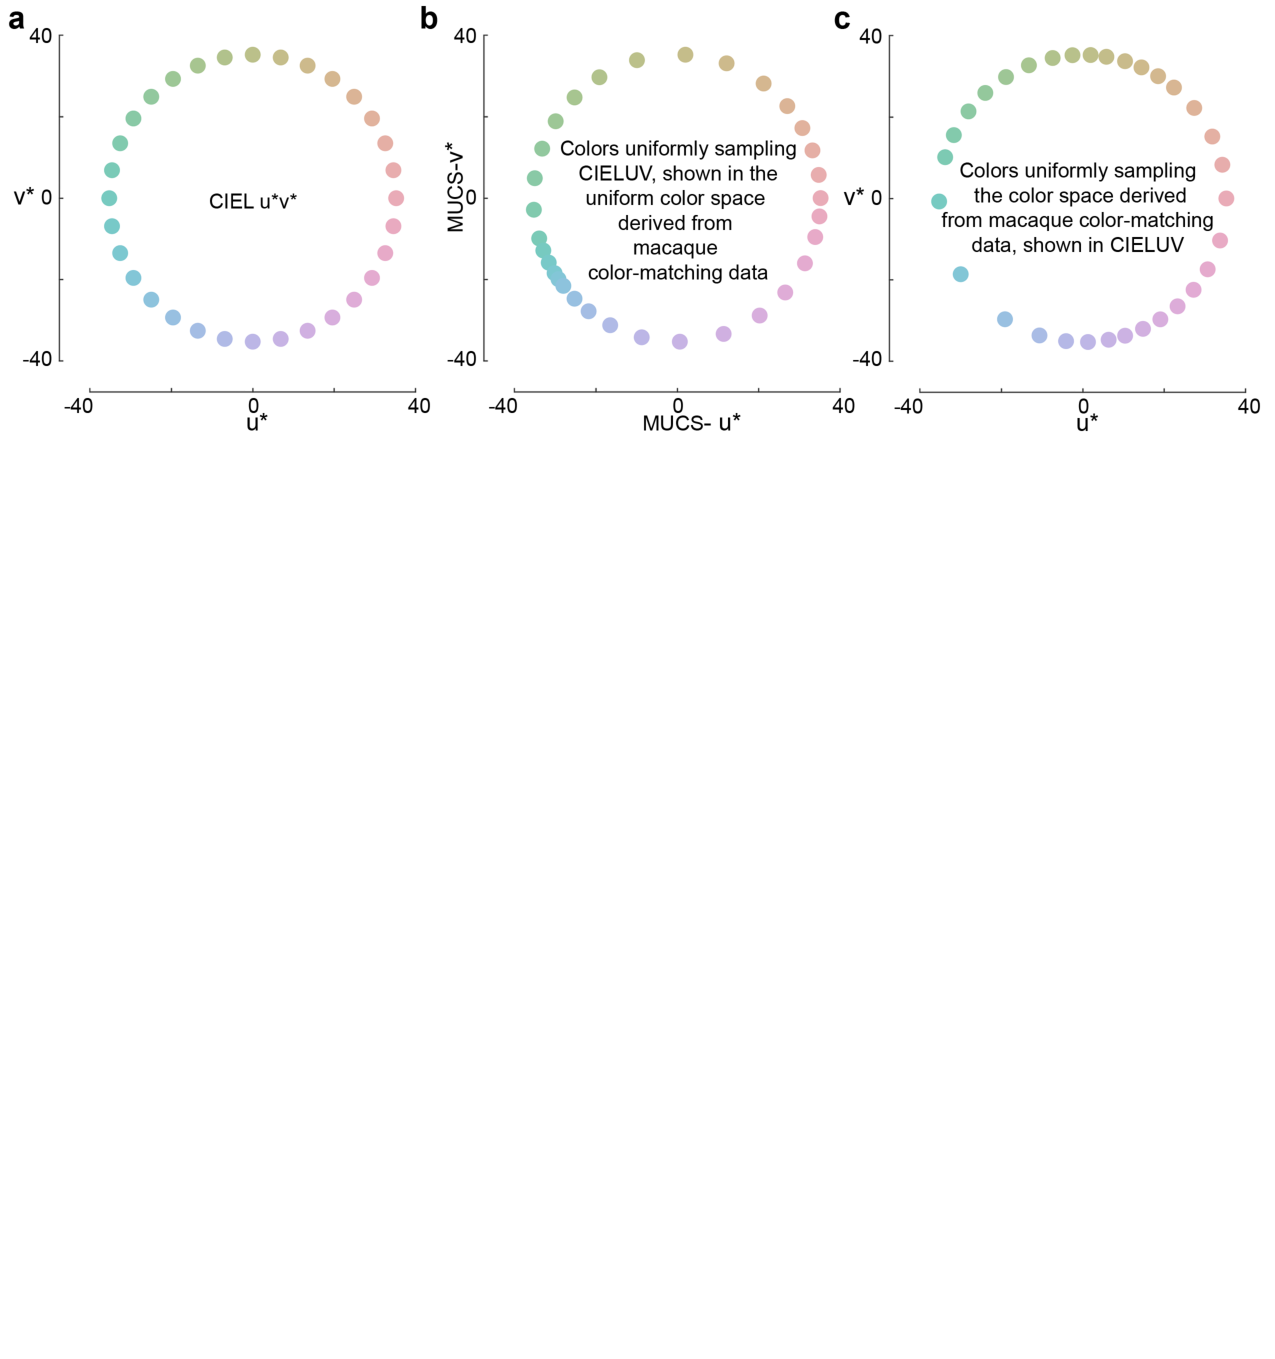
\includegraphics[width=\textwidth+4cm,trim={0 15cm 0 0},clip]{Outputs/Paper/Figures/flat/F6_ColSpace_2}
           \caption{\textbf{Perceptually uniform color space derived from the color-matching data in macaque monkeys.} 
			\textbf{a}, CIELUV color space with 64 color samples at even intervals in hue angle. 
			\textbf{b}, The same color samples plotted in the uniform color space derived from macaque monkeys; note that the axes are not CIELUV but MUCS (macaque uniform color space). 
			\textbf{c}, Colors sampled evenly from the uniform color space derived from macaque monkeys, projected into CIELUV.}
		\label{fig:MACBEHcolorspace}
    \end{fullwidth}
\end{figure}

\paragraph{A perceptually uniform color space unconfounded by language}

Ample behavioral and neurophysiological data support the hypothesis that the perceptual systems that enable color vision are similar in macaques and humans \citep{schnapf_spectral_1987,gagin_color-detection_2014,horwitz_what_2015,lafer-sousa_color-biased_2016}. 
The weight of this prior evidence gives us confidence that the present results obtained in monkeys also apply to humans. 
That is, it seems likely that the CIELUV color space is not perceptually uniform for human observers either, which aligns with the findings of others \citep{stockman_colorimetry_2010,judd_ideal_1970,bujack_non-riemannian_2022}. 
The non-uniformities in CIELUV and other nominally uniform colorspaces likely have multiple sources; in many cases such colorspaces are strongly constrained to have a small number of parameters, and are designed with very specific viewing conditions in mind.
A task such as ours, paired with a stimulus-space non-uniformity TCC-v model gives a method by which a minimally constrained uniform colorspace may be created.
To the extent to which language is a factor in producing color-space non-uniformities, the behavioral data in macaques provide an opportunity to reconstruct a uniform color space unconfounded by language, which may provide a useful insight into colorspace progression along the visual pathway in humans. 

To generate such a space, we computed, empirically, a transformed color space such that the macaques would, on average, show no choice bias. 
We refer to this space as the Macaque Uniform Color Space (MUCS). 
When colors evenly sampled from the CIELUV space (Figure 6a) are plotted within this macaque-derived uniform color space, colors are bunched around the teal part of the space, and to a lesser extent, around the peach-colored part of the space (Figure 6b). We can also take colors sampled at uniform intervals in MUCS and project them into CIELUV (Figure 6c). 
This arrangement shows relative bunching around lime colors and lavender colors, which correspond to the colors of the poles of the S-cone-opponent axes. 
These results provide clues to the origin of the stimulus space non-uniformity in CIELUV.

At present our "colorspace" has only minimal coverage - it only considers colors which are isoluminant and in a ring which was originally specified in CIELUV.
Using it beyond a very specific range of applications would require extrapolation, either through cautious mathematical extrapolation or through the collection of new data determined by the need at hand.

\paragraph{Discussion}

Throughout this paper, our linking of cognitive biases to color categories has relied heavily upon the conclusion of \citet{bae_stimulus-specific_2014} that categorical processing of color results in biases towards color category centers.
While this seems like a reasonable hypothesis, supported by the evidence so far, it seems likely that as future research is conducted additional nuance will be added to this picture, which may in turn refine our understanding of the experiments reported here.
For example, it is currently unclear to what extent biases are driven by attractor points versus repellor points - to our knowledge there has so far been no study which has been able to separate these two potential mechanisms.
Further, almost all work we are aware of (with the partial exception of \citet{muchhala_does_2022}) has limited the stimulus space to a set of isoluminant and isosaturated colors - this is an understandable and practical compromise but clearly leaves a great deal to be desired.
We are hopeful that new techniques might soon allow for the collection of data which more comprehensively explores the connection between attractor points and color categories.

We conclude from the current results that monkeys do not have color categories.
Some enthusiastic reviewers would like us to consider non-linguistic possibilities and have provided two for our consideration: (1) Perhaps monkey cognition is different in how sensory signals are processed to form categories in a fashion which means they are not recovered in our task, (2) that macaques are born with innate color categories, but that our particular macaques lost them at some point in their development.

To the first possibility: monkeys have similar cones, similar color-detection thresholds (if anything more sensitive than humans, see \citep{gagin_color-detection_2014}), similar visual cortex (up through the ventral visual pathway, see \cite{lafer-sousa_color-biased_2016}), and show similar attentional mechanisms to humans, all of which suggest that alternative explanations cannot be found in the normal operation of the visual system. 
This leaves differences in cognition, which is the explanation we appeal to, to explain the results. 
We believe that this is semantically equivalent to the claim we are making.

To the second possibility: we agree that many innate behaviors require appropriate developmental experience to be expressed as adults. 
It is possible that the animals have innate color categories and that they do not have the appropriate environmental or other experience to retain these. 
We very much doubt that this has occurred in this case. 
The animals live in social colonies with lots of enrichment - they eat natural fruits and have many colored toys. 
While this is not "nature", it provides sufficient experience for the expression of every other measured cognitive behavior in the animals (including memory, face recognition, vocalization, etc.). 
As far as we are aware, the developmental literature indicates that this environment is permissive of the expression of innate behaviors, and that there must be radical limitations in the environment for innate behaviors to be lost - for example deprivation of face exposure.

The mixture-model results in macaque monkeys are strikingly different from those in humans, but are similar in one regard: they both show repeller points aligned with the poles of the S-cone axis (compare the zero-crossings of the positive slopes in Figure 1e with those in Figure 2c; SI Figure 2) \citep{skelton_biological_2017,bae_why_2015,panichello_error-correcting_2019}. 
This commonality supports the idea that the present results apply to the human case, and suggests that the non-uniformity in CIELUV arises because the contribution of S-cone signals to supra-threshold color matching (in monkeys or humans) has not been accurately estimated. 
Such an inaccuracy may reflect differences between threshold measurements (such as were used in the measurement of the CIE standard observers, the data from which was subsequently used to develop colorspaces such as CIELUV) versus appearance measurements (such as those made presently), along with differences in the neural circuits that handle S versus L/M signals \citep{RN655, conway_color_2014}. 

We have thus far worked on the assumption that cognitive biases (represented by offsets in responses) and stimulus-space non-uniformities are fundamentally different mechanisms - one active and purposeful, and the other an unintended side-effect of how we define colorspace.
Taken this way our study shows that there are differences between monkeys and humans in high-level processes: humans show consensus color categories and monkeys do not. 
But it is also plausible that the relationship between these two mechanisms is less clear-cut; could it be that stimulus-space non-uniformities (perhaps task-dependent ones) are also an active mechanism by which beneficial biases might be introduced?
Further work will be required to understand how these mechanisms might interact, and to what extent each exists with purpose.

The present results are consistent with the idea that color ordering and the capacity to form color categories are innate - if the monkeys showed no capacity for color ordering, their pattern of errors would be entirely random and there would be no structure in the similarity matrices, i.e. the matrices would be uniform across the whole square and wouldn't show strong clustering along the diagonal. 
But contrary to longstanding arguments in empirical philosophy \citep{RN18743}, the present results imply that perception by itself is not sufficient to generate consensus color categories. 
Prior work with congenitally blind people has shown that color perception is unnecessary for people to generate rich conceptual knowledge of color, including color categories \citep{kim_shared_2021}. 
The prior work and the present work taken together show that perception is neither necessary nor sufficient for the emergence of consensus color categories, and consensus color categories are therefore likely not innate. 

If color categories are not innate, where do they come from? 
Color categories appear to reflect the behavioral relevance of colors in the world \citep{RN18616,gibson_color_2017}; the relevance of things is partially culturally determined, introducing a role for language in shaping consensus color categories. Given that color categories can be learned, as clearly evident in at least one macaque in our study (Figure 5) and two macaques in another study \citep{panichello_error-correcting_2019}, the introduction of language provides a mechanism by which cultures can form consensus about color categories. 
For example, universal patterns in color naming predict which parts of scenes are labeled as objects \citep{gibson_color_2017}. 
We speculate that the choice biases in humans will partially reflect the stimulus-space non-uniformities observed in monkeys as well as cognitive biases that have achieved consensus through shared behavioral relevance communicated by language \citep{RN18511,RN18514,RN18602}. 


\printbibliography[title=Main Text References]
\end{refsection}

% DON'T EDIT. If "endfloat" option is enabled all floats appear before appendices
\if@endfloat\clearpage\processdelayedfloats\clearpage\fi 

\begin{refsection}
\newpage

\section{Methods}

\subsection{Subjects}

Data were collected in four adult male rhesus macaques (Macaca mulatta)("PO, CA, BU, and MO") weighing 8–10 kg. 
All experimental procedures were approved by the Animal Care and Use Committee of the National Eye Institute and complied with the regulations of the National Institutes of Health. 
Plastic headposts were mounted with sterile surgical procedures, using procedures described in detail elsewhere \citep{lafer-sousa_parallel_2013}. 
The animals were acclimatized with positive reinforcement to sit in a custom-made chair positioned with the eyes 70cm in front of a computer monitor and to perform visual tasks as described below. 
At the beginning of each testing session, we positioned a mouthpiece to deliver fluid reward to the animal. 
An infra-red camera was directed at the eye to monitor eye position with the ISCAN system. 
The precision of the eye tracking was \textasciitilde0.3\degree{}. 

\subsection{Behavioral task}

The animals were trained to perform a 4-Alternative Forced Choice (4-AFC), Delayed Match to Sample task, in which they were shown a colored cue and rewarded for selecting the match option that had the identical color (see Figure 1). 
The colors, described in more detail below, were drawn from a set of 64 colors that evenly sample hue angle of CIELUV color space \citep{stockman_colorimetry_2010}. 
Each trial was initiated when the animal fixated a small cross at the center of the screen; trials were aborted if the animal did not maintain fixation until the fixation cross disappeared toward the end of the trial. 
Fixation was defined as within a 1.5\degree{} wide area centered on the fixation cross, well within the precision of the eye tracker.
The trial sequence was as follows. 
50 ms after initiating the trial by fixating the central cross, a 3\degree{}-diameter "cue"  of a color randomly drawn from the set of 64 colors appeared for 750ms. 
The cue was positioned on the monitor at the same location for all trials during a given daily recording session.
From day to day, the position of the cue could vary, from 2.5\degree{} to 6\degree{} eccentricity (measured at the center of the cue) and be at any angle from fixation.
The cue was followed by a gray screen for a brief "memory" period of 600-900 ms, after which four match options appeared along an arc at an eccentricity of 6\degree{}. 

One match option was always a direct match to the cue, and the other three were randomly sampled without replacement from the remaining 63 stimuli. 
The match options had the same shape and size as the cue (3\degree{}-diameter discs); they were evenly spaced along the arc, with a gap of 2\degree{} separating each option. 
In all animals except one (CA), the arc along which the match options were placed was in the visual hemifield opposite to the cue. 
The exact position of the arc within the hemifield varied from trial to trial, so the animals could not anticipate where the choice options would appear. 
Animal CA had a small scotoma spanning \textasciitilde3\degree{} of visual angle in a quarter of the visual field as the result of a \textasciitilde3 mm diameter V1 lesion, so the cue and choices were placed in the same (intact) hemifield, taking care to avoid overlap of the position of the cue and the choices. 

After a random period from 500-1000 ms, the fixation cross disappeared, instructing the monkey to direct its eyes to one of the choices. 
This random period helped guard against the animals making impulsive responses because they could not anticipate when exactly the choice options would appear. Reward was given only if the animal selected with an eye movement the choice that was identical to the cue. 
If the monkey failed to make a choice within 5 seconds or broke fixation at any point before the termination of the fixation cross, the trial was aborted.

The experiment was controlled with custom software written in MATLAB and Psychtoolbox \citep{kleiner_whats_2007}.

\paragraph{Stimuli}
Stimuli were 3\degree{} diameter discs presented on a Cambridge Research Systems Display++ screen. 
Colors were defined to be on an equiluminant plane in CIELUV color space, with the luminance matched to the adapting gray background (L* = 76.0693, 38.5 cd/m$^2$; adapting field chromaticity was xy\textsubscript{1931}: 0.2684, 0.2409). 
The stimulus set included 64 colors, evenly sampling CIELUV hue angle (5.625\degree{} between adjacent stimuli), of equal CIELUV saturation (radius 37), the highest saturation possible for a set of stimuli of equal saturation and luminance given the gamut of the display.
Luminance contrast noise was randomly added to each pixel of the cue and the match options to mitigate chromatic aberration. 
The luminance added to each pixel was updated every frame and drawn uniformly from a continuous range of +/- 5 L* units (the resulting stimulus looks like a colored disc viewed behind a thin veil of television snow). 
CIELUV was used to define the stimuli because it has an associated chromaticity diagram, but the stimuli can readily be transformed into other spaces such as CIELAB and DKL. 

The color stimuli corresponding to the poles of the cone opponent cardinal axes, labeled in the polar mixture model plots, were computed as follows. 
CIELAB and CIELUV values were transformed to XYZ coordinates using the PsychToolbox functions "LabToXYZ" and "LuvToXYZ" respectively.
An XYZToLMS matrix was constructed using MATLAB's "mldivide" function with the Smith-Pokorny cone fundamentals and the CIE XYZ standard observer color matching functions as inputs.
The PsychToolbox function "ComputeDKL\_M" was then used to compute a conversion matrix for converting between LMS and cone opponent cardinal axes that define the DKL colorspace. 
The code which accomplishes the above is available \href{https://github.com/NEI-LSR/MacaqueColorCategories/blob/main/Analyses/DKL/computeDKL_XYZ.m}{here}.

\paragraph{Human Data}

Data from published reports using two related tasks completed in human subjects were kindly provided by Gi-Yeul Bae \citep{bae_why_2015} and Timothy Buschman \citep{panichello_error-correcting_2019}.
Both these data sets involved a paradigm in which participants matched the color of a cue to a ring of colors showing a continuous progression of colors around the color circle (a "color wheel"). 
The results of the two prior studies are consistent with each other: when analyzed with a mixture model, both data sets show four color categories corresponding to blue, green, orange, and pink (SI Figure 1); moreover, the results on a version of the task that omits the memory delay period also recover these four color categories \citep{bae_why_2015}.
This prior work shows that the results on the color-matching task are reproducible and robust. 
It is therefore likely that the results of the present version of the task, which is distinguished from the prior work by providing as options discrete targets as opposed to a continuous colored wheel, would also be similar. 

But to test this likelihood, we recruited human participants via Amazon Mechanical Turk to perform the same task used in the macaque monkeys in the present work. 
To request a trial, participants used a mouse to adjust the location of a cursor to click on a fixation cross, after which a cue was shown to one side of the fixation cross, and the cursor disappeared. 
The cue was displayed for 750 ms. 
After the cue was extinguished, a fixation cross was shown but the cursor remained hidden to de-incentivize mouse movement (1500 ms). 
Four choices were then shown, and the cursor reappeared; participants made their selection by using the mouse to move the cursor to their choice and clicking the mouse. 
Most other aspects of the experimental design were the same as the experiment deployed with the monkeys: 64 colors of equal saturation and luminance (we assumed the monitor that each on-line participant was using matched the sRGB standard), evenly sampling CIELUV. 

We did not provide feedback to human participants (in line with prior human work \citep{bae_why_2015,panichello_error-correcting_2019}). 

We collected data from 72 participants in blocks of 400 trials; 400 - 2000 trials from each (mean: 639 trials).

The pattern of results was consistent with the published studies using the continuous ring of colors, recovering four significant color categories corresponding to blue, green, orange, and pink (SI Figure 1). 

\subsection{Data Analysis}

\paragraph{Psychometric functions}

Psychometric functions (see Figure 2a, SI Figure 2) were estimated with a Weibull cumulative density function: %!!!!

\begin{equation} \label{eq:Weibull}
    y=\zeta+(100-\zeta-\gamma) *\left(1-e^{-(\omega / \lambda)^k}\right) 
\end{equation}

Where animal performance (y) is a function of trial difficulty ($\omega$), computed for each trial as the angular difference between the color of the cue and the color of the foil with the closest color to the cue. 
The other parameters are the floor of the function ($\zeta$), the ceiling ($\gamma$), slope ($\lambda$), and inflection point ($k$). 
All completed trials were included in the analysis of the psychometric functions. 
The number of completed trials for each animal were: 76121 (PO); 54555 (CA); 24526 (BU); 54252 (MO). 

\paragraph{Mixture Modeling}\label{para:MixtureModeling}

Following experiments in human subjects, we analyzed the distribution of color matches made to each color using a mixture model \citep{zhang_discrete_2008,bae_why_2015}; this model assumes that the shape of the distribution is normal and provides an estimate of the width of the distribution, the offset (or bias) of its peak relative to the target color, and the guess rate.
Prior work has done this analysis with a von Mises distribution \citep{zhang_discrete_2008,bae_why_2015}.
We found it simpler to implement it with a Gaussian function, $f(\theta)$:

% demo annotated-equation code from here: https://mirrors.concertpass.com/tex-archive/macros/latex/contrib/annotate-equations/annotate-equations.pdf

%\newpage %Sometimes the annotations don't show up, the hacky solution is to force them onto a new page

\begin{equation} \label{eq:GaussianEquation}
    f(\theta) = {\alpha} \cdot e^{-\frac{(\theta-{\mu})^2}{2{\sigma}^2}} + {\zeta}        
\end{equation}

% \vspace{2em} 
% \begin{equation} \label{eq:GaussianEquation}
%     f(\theta) = 
%     \eqnmarkbox[purple]{alpha}{\alpha}
%     \cdot
%     e^{
%     -\frac{(x-
%     \eqnmarkbox[violet]{mu}{\mu}
%     )^2}{2 
%     \eqnmarkbox[blue]{sigma}{\sigma}^2}}
%     +
%     \eqnmarkbox[gray]{zeta}{\zeta}        
% \end{equation}

%\annotate[yshift=1em]{above,left}{alpha}{height of the curve's peak}
%\annotate[yshift=1em]{above}{mu}{position of the center of the peak}
%\annotate[yshift=-0.75em]{below,left}{sigma}{standard deviation}
%\annotate[yshift=-1em]{below}{zeta}{floor}
%\vspace{2em} 

where $\alpha$ is the height of the curve's peak, $\theta$ is the hue angle, $\sigma$ is the standard deviation (width), $\mu$ is the center of the peak (so the offset is $\theta$-$\mu$), and $\zeta$ is the floor (guess rate). 
To do the analysis, we used the MATLAB fit function, which was provided with the number of times each choice color was an option for the given cue across all completed trials and produced the best-fitting function along with the 95\% CI values for those parameters (SI Figure 3; note that the tails of the distributions in SI Figure 3 reach an asymptotic floor, justifying the use of the simpler Gaussian fitting procedure). 
The offset values for each cue were smoothed with a moving average spanning three colors (16.875\degree{}) (Figure 2b and 2c, Figure 5a, and SI Figure 4). Negative-slope zero-crossings in which the 95\% CI exceeded the zero-crossing were considered category centers (see Figure 1).

The width of distribution of matches varied among the colors; this was also observed by \citet{bae_why_2015} (see their Figure 7). 
This variation implies that the assumption of uniformity of the colorspace is not valid. 
Moreover, such a non-uniformity could yield an offset in the mixture model (see Figure 3), so any offsets recovered by the mixture model need not require a cognitive origin.  
The alternative hypotheses for the origin of offsets recovered by the mixture model (a cognitive origin versus a stimulus-space non-uniformity), prompted us to analyze the data with a more sensitive model, the Target Confusability Competition model \citep{schurgin_psychophysical_2020}.
We recognize that in principle, the mixture model could distinguish these alternative hypotheses, but we encountered some limitations using the mixture model that were readily overcome by the TCC model. 

\paragraph{Modified Target Confusability Competition Model (TCC-v)}\label{para:TCC}

The key elements of the TCC model are a similarity function, which determines the similarity between stimulus $s_i$ and stimulus $s_j$ through a non-linear mapping of distance in colorspace to perceptual similarity, and a value of $d'$, which can be thought of as describing the amount of noise acting in the system. 
These two elements can be used to predict the probability that a choice of colour $s_j$ will be picked from the set of $\left[s_{j1}...s_{jn}\right]$, on a trial where the cue is $s_i$. 

The probability of a particular choice being selected on a particular trial ($p_t(\text{selected choice} = \text{choice}_n)$) is dependent on the cue, the set of choices, the similarity function ($f(\theta)$), the value of $d'$, and the perceptual distances between stimuli ($D$).

\begin{equation} \label{eq:pt}
    p_t\left(\text{selected choice} = \text{choice}_n \mid \text{cue},\text{choices}_{i:j}, f(\theta), \delta, D\right)
\end{equation}

where $f(\theta)$ is the Gaussian equation (\autoref{eq:GaussianEquation}), $\delta$ is the value of $d'$, and $D$ is the perceptual distances between stimuli.

The TCC model has been deployed with the assumption that the colorspace is perceptually uniform \citep{schurgin_psychophysical_2020}; this assumption is implemented as a single similarity function fit for all stimuli. 
But, as \citet{schurgin_psychophysical_2020} demonstrate the similarity function need not be fixed (see their Figures 1d and Extended Data Figure 5). 
Our implementation of the model, which we call TCC-v, permits the similarity function to vary for each cue (the "v" is for vary). 

We created four versions of the TCC-v model: the "null" model (with only parameters for the Gaussian width of the similarity function and $d'$, and thus no allowance for bias), the "cognitive bias" model (with 64 parameters corresponding to offset values shifting the peak of the similarity function for each stimulus to higher or lower hue angles, in addition to $d'$ and gaussian width), and the "stimulus-space non-uniformity model" (with 64 parameters corresponding to the relative distance between each pair of neighboring stimuli, in addition to $d'$ and gaussian width). 
Finally, the "free-similarity" model, does not pre-suppose any specific similarity function; every cell in the similarity matrix is an independent parameter. 
This flexibility allows for patterns of similarity that are not captured by our hypotheses. 

In fitting the model parameters, our goal is to minimize the negative log likelihood (NLL) of the observed data. 
The NLL is computed as the sum of the negated log of the probabilities of the choices that were selected being selected. 

\begin{equation}
    \text{NLL} = \operatorname{sum}\left(-\left(\log \left(p_t\left(\text {selected choice} = \text{choice}_x\right)\right)\right)\right)
\end{equation}

where $\text{choice}_x$ was the choice that was selected on each trial.

The parameter estimates for the free parameters used by the model are iteratively updated until the model reaches a stable minimum NLL. 

The "null" model is defined by $f(\theta)$ (where $\alpha$ = 1, $\zeta$ = 0, $\mu$ = 0, $\sigma$ is 1 free parameter) and $d'$ (free parameter), and assumes $D$ to be uniform. 
The "cognitive bias" model is defined by $f(\theta)$ ($\alpha$ = 1, $\zeta$ = 0, $\mu$ is 64 free parameters, $\sigma$ is 1 free parameter) and $d'$ (free parameter), and also assumes $D$ to be uniform. 
The "stimulus-space non-uniformity" model is defined by $f(\theta)$ (where $\alpha$ = 1, $\zeta$ = 0, $\mu$ = 0) and $d'$ (free parameter), but specifies for each pair of neighboring stimuli a unique value for $D$ (64 free parameters). 
Note that the cognitive bias model and the stimulus-space non-uniformity have the same total number of free parameters (66). 
The "free similarity model" is not defined by $f(\theta)$; it is defined by $d'$ and the similarity matrix. 
The similarity matrix is defined by 4096 ($64^2$) parameters, one for each combination of cue and possible choice (note that the free similarity matrix is not required to be symmetric).
In practice, when fitting a free similarity model we fix $d'$ rather than allowing it to be a free parameter.

$p_t(\text{selected choice} = \text{choice}_n)$ is the probability that a sample drawn from an independent normal distribution $(X_i \sim N)$ is the highest of such samples drawn for all the choices ($i:j$) on a particular trial. 
The mean ($m$) of each distribution is defined by the similarity value for that cue/choice combination, multiplied by $d'$, and has a variance of 1.

\begin{equation}
    p\left(\text{selected choice} = \text{choice}_n\right) = 
    p\left(X_i \sim \mathcal{N}\left(m_n \cdot \delta, 1\right)
    >\max 
    \left(X_{i+1: n} \sim \mathcal{N}\left(m_n \cdot \delta, 1\right)\right)\right)
\end{equation}

where $m_{i:j} = f\left(|\text{cue}_{i} - \text{choices}_{i:j}|\right)$, and $\delta$ is the value of $d'$.

We used an AFC paradigm as opposed to a continuous response space, so we can take advantage of an alternative computational method for estimating $p_t(\text{selected choice} = \text{choice}_n)$, using correction factors provided by \citet{mcgraw_common_1992} (their Table 3). 
This decreases the amount of time taken to fit the TCC-v models. 
The method for computing $p_t(\text{selected choice} = \text{choice}_n)$ in the original TCC model of Schurgin et al. is provided here: \verb|modelPDF| in \verb|TCC_Code_InManuscriptOrder |\verb|\Model| \verb|\TCCUncorrelated.m| from \url{https://osf.io/j2h65/}. 
The method we used is provided here: \url{https://github.com/NEI-LSR/TCC_AFC}.

When fitting the free similarity matrix model, we fix $d'$ to provide a constraint on the floor and ceiling of values in the similarity matrix.
$d'$ is strongly correlated with the range of the values in the similarity matrix; the range of similarity values in the similarity matrix has a maximum span of 0 to 1. 
Equivalent NLL values can be obtained either by restricting the range (e.g. 0.49 to 0.51) and a high value of $d'$ (e.g. 20), or by having a larger range (e.g. the full 0 to 1) and a low value of $d'$ (e.g. 0.1). 
If $d'$ is not fixed, the model is as likely to assume a restricted range as it is a larger range (though still bounded between 0 and 1) but will take a long time to converge. 
Fixing $d'$ impacts the specific values (akin to increasing or decreasing the contrast of the similarity matrix image) but it does not impact the interpretation of the similarity matrix. 
We chose a $d'$ value of 1 which is a reasonable estimate for our task \citep{schurgin_psychophysical_2020}.

In the original TCC model, the similarity function uses two parameters that define a Gaussian function representing perceptual noise and an exponential function; these two functions are convolved (see Figure 1f of \citep{schurgin_psychophysical_2020}). 
We simplify the similarity function such that it is defined by a Gaussian alone. 
The cost of this is that it does not allow for a distinction between the impact of perceptual noise (where the curve flattens off approaching perceptual distances of 0) and similarity (the general shape of the function). 
In practice, we found that these parameters were highly correlated, and that reduction to a single parameter substantially reduced the computational cost of model fitting, and produced parameter estimates that were more resistant to variation in model-fitting starting values. 
This simplification also made it easier to modify the model; for example, to allow for the peak of the function to not be at 0 (this affords the TCC-v model the same ability as the mixture model to capture offsets).

\paragraph{Choice Probability Matrices vs. Similarity Matrices}

\begin{figure}
    \begin{fullwidth}
    \centering
      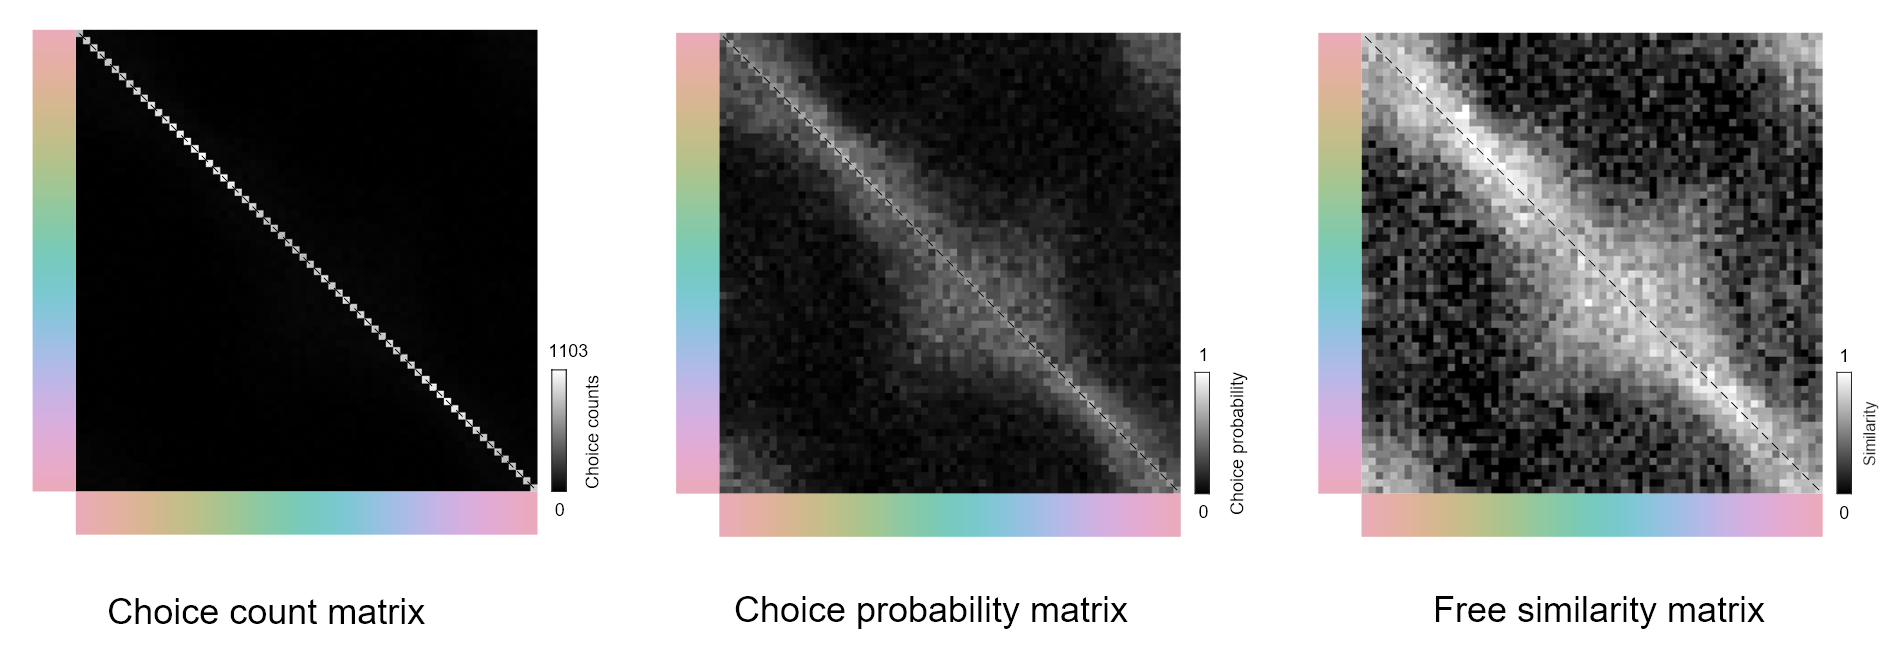
\includegraphics[width=\textwidth+4cm]{Outputs/Paper/Figures/flat/F7_choiceProbVsSim.png}
           \caption{\textbf{Comparison of Choice Count Matrices, Choice Probability Matrices, and Similarity Matrices}.
           Choice count matrices describe the number of times a specific choice is made. 
           Choice probability matrices normalise for the number of times a particular choice was available as a choice option. 
           Similarity matrices are created through model fitting and represent the perceptual similarity between stimuli, and are beneficial since they are not influenced by mixed viability of distractors (see text for further details).
           Plots shown are for the combined monkey data. For individual data, see Figure S5 and S6.}
		\label{fig:choiceProbVsSim}
    \end{fullwidth}
\end{figure}

A choice probability matrix is a graphical representation of the probability that choice $y$ will be chosen given cue $x$.
To construct such a matrix, one counts the choices which were made in response to each cue, producing what we can refer to as a choice count matrix, and then divides each cell by the number of times that each cue/choice combination was presented. 
This normalizes for the possibility that some cue/choice combinations were presented more than other combinations. 
This process disregards any information about what the unchosen distractors were on a given trial.

In paradigms which use a continuous response space the set of choices is the same on each trial – the full set of possible choices. 
This is not the case for our reduced AFC paradigm, and this introduces a potential issue which needs consideration.

Imagine a trial with three distractors which are all close to one another (let's say that they are 5, 6, and 7 colorimetric units away from the cue).
On another trial, imagine that one distractor is a much more viable choice option than the other two (let's say the choices are 5, 25 and 26 units away from the cue).
The odds of picking the distractor that is 5 units away is different on these two trials - it is more likely on the second trial, because the other distractors are less viable options. 
This becomes a potential issue because to counterbalance trials such that each cue is shown with the full set of possible distractors would require roughly 2.5 million trials (nchoosek(63,3) * 64).
Without counterbalancing, it is not possible to disentangle differences in choice probability which arise due to perceptual similarity (which is what we are aiming to measure) vs differences in distractor viability.

We avoid having to collect a complete set of 2.5 million trials by employing the concept of a similarity matrix.
A similarity matrix is the core component of a TCC-v model, and maps the similarity between cues and choices. 
Using it, the similarity between the cue and each of the choices on a particular trial (and also the similarity between each of the choices themselves) can be used to compute the probability of each choice being selected.
While we can compute the choice probability matrix rather simply, as described above, the creation of a similarity matrix requires a model-fitting approach – a similarity matrix is randomly initialized with values, and the likelihood of the data given that matrix is computed, then the matrix is randomly perturbed and the likelihood of the data is recomputed, and then perturbed again in whatever directions seem to increase the likelihood of the data, setting forth an iterative process whereby the similarity matrix is perturbed until a maximum in likelihood is reached, and our best estimate of the underlying similarity matrix is thus settled upon.
This is a computationally intensive process, and for datasets with many choices (such as those with a continuous response space), we have been unable to fit similarity matrices. 
Thankfully, there is a trade-off: data collected with continuous response spaces see less benefit of a similarity matrix over a probability matrix. 
For such datasets, as the number of trials increases the probability matrix increasingly approximates the similarity matrix.
It is expected that choice probability matrices and similarity matrices will be highly correlated and show the same structure.

A related issue, also addressed by employing the concept a similarity matrix, is the artifact caused by the inclusion of a direct match on every trial in our paradigm. 
This can be thought of as an unequal counterbalancing which no number of repeated trials would be able to balance out, but it is necessary for our training of the monkeys (since there needs to be a clear rubric for what choices are "correct" and thus rewarded).
Note how the choice count matrices and choice probability matrices for our data appear to show an elevated diagonal. 
The reason this exists in the choice count matrix is clear – those option are simply presented more frequently, but the reason this survives the normalization (by the number of times that each cue/choice combination was presented) is less obvious: any non-match choice which is close to the direct match will always have a viable competitor (the match), whereas the match choice won't always have a viable competitor (since it is possible that the distractors are all distant on a particular trial).
This leads to an increased probability of selecting the matching choice relative to an incorrect choice. This issue only affects choice probability matrices; it does not affect similarity matrices.

\paragraph{Quantitative Model Comparison}
To compare the relative performance of models, we computed Bayesian Information Criterion (BIC) values for each model from the NLL. 
The BIC values provide a unit by which we can assess whether the differences between NLL are meaningful, penalizing for number of parameters and number of trials. 
BIC also allows us to compare models with differing numbers of parameters (though note that the "cognitive bias" and "stimulus-space non-uniformity" models have the same number of parameters).

\begin{equation}
    \text{BIC} = k\ln(n)-2\ln(\hat{L})
\end{equation}

Where $\hat{L}$ is the maximised likelihood of the model, $n$ is the number of trials, and $k$ is the number of parameters.

To compare the relative performance of the cognitive bias and stimulus-space non-uniformity models we performed 100 bootstrap iterations of the analysis. 
Each bootstrap drew 24526 trials from the total number of completed trials for each animal (24526 was the minimum number of trials of completed trials among the 4 animals). 
Both models were then fit to each bootstrap iteration, and the BIC values were computed (see Figure 4d).

\paragraph{Reverse-engineering a uniform color space from the macaque color-matching data}

The present results imply that CIELUV is perceptually non-uniform; that is, that it samples with variable density the true underlying perceptual colorspace. 
The parameters of the stimulus-space non-uniformity model describe the relative positions of the stimuli, as determined empirically. 
After converting from inter-neighbor relative distances to polar angles, these can be thought of as the hue angles for the stimuli that we used, represented now in a behaviorally derived color space which we refer to as the Macaque Uniform Color Space (MUCS) (Figure 6b). 
The inverse transformation is also possible; we can define a set of hue angles that are uniformly distributed in MUCS and convert them into CIELUV. 
For example, if we define hue angle $i$ in MUCS, we can reparameterize that hue angle such that it is defined by its angle relative to the two experimental stimuli on either side of it (hue angle $i$ is at y\% of the angular distance on the path between experimental stimuli $a$ and $b$). 
We can then plot MUCS hue angle $i$ in CIELUV by plotting it at the location which is y\% along the path between experimental stimuli $a$ and $b$ in CIELUV. 
Such a set of hue angles is shown in Figure 6c. 

The MATLAB script MUCS.m will generate a user-defined number of colors sampled evenly from the behaviorally generated color space.


\printbibliography[title=Methods References]
\end{refsection}

\section{Acknowledgments}

Joshua Fuller-Deets adapted code from Shay Ohayon to create the experimental paradigm; Rosa Lafer-Sousa collected pilot data; Whitney Teagle and Shriya Awasthi assisted data collection. 
Funding was provided by the Intramural Research Program of the National Eye Institute. 
We are thankful to the animal care team lead by Denise Parker and Hayden Warnock and to the veterinary staff of the NEI for excellent animal care. 
We thank members of the Laboratory of Sensorimotor Research, attendees of the Colour Group of Great Britain’s January Vision Meeting (2022), the Vision Sciences Society (2022, 2023), the Society for Neuroscience (2023), and the Color Workshop sponsored by the University of Giessen (Summer 2023) for helpful feedback. 
We thank Thorsten Hansen and David Brainard for consultation on color conversions, Ramon Bartolo for mathematical assistance, Hendrikje Nienborg, Christian Quaia, Corey Ziemba, and anonymous reviewers, for comments on the manuscript, and Karl Gegenfurtner for the initial prompt to think about testing for color categories in macaques.

\section{Author contributions}

% table? e.g. https://twitter.com/AnneEUrai/status/1361356189284581387
% made previously, Danny didn't have the headspace to show to Bevil: https://github.com/NEI-LSR/MacaqueColorCategories/commit/8b63cd3800d6faa46e5404dd7c43a1fee113a8b5
% 'CRediT' (https://casrai.org/credit/)

Conceptualization: BRC, DJG\newline
Data curation: DJG\newline
Formal Analysis: DJG, HMS, ALYC\newline
Funding acquisition: BRC\newline
Investigation: all authors\newline
Methodology: all authors\newline
Project administration: BRC\newline
Resources: BRC\newline
Software: DJG, HMS, ALYC\newline
Supervision: BRC\newline
Validation: DJG\newline
Visualization: all authors\newline
Writing – original draft: BRC, DJG\newline
Writing – review \& editing: BRC, DJG\newline


%%%%%%%%%%%%%%%%%%%%%%%%%%%%%%%%%%%%%%%%%%%%%%%%%%%%%%%%%%%%
%%% SUPPLEMENTARY MATERIAL / APPENDICES
%%%%%%%%%%%%%%%%%%%%%%%%%%%%%%%%%%%%%%%%%%%%%%%%%%%%%%%%%%%%

% modified from: https://tex.stackexchange.com/a/611819/169285
\newcommand{\supplementarysection}{%
  \setcounter{figure}{0}% Reset figure counter
  \let\oldthefigure\thefigure% Capture figure numbering scheme
  \renewcommand{\thefigure}{S\oldthefigure}% 
}

\supplementarysection

\begin{figure}
    \centering
    \begin{fullwidth}
    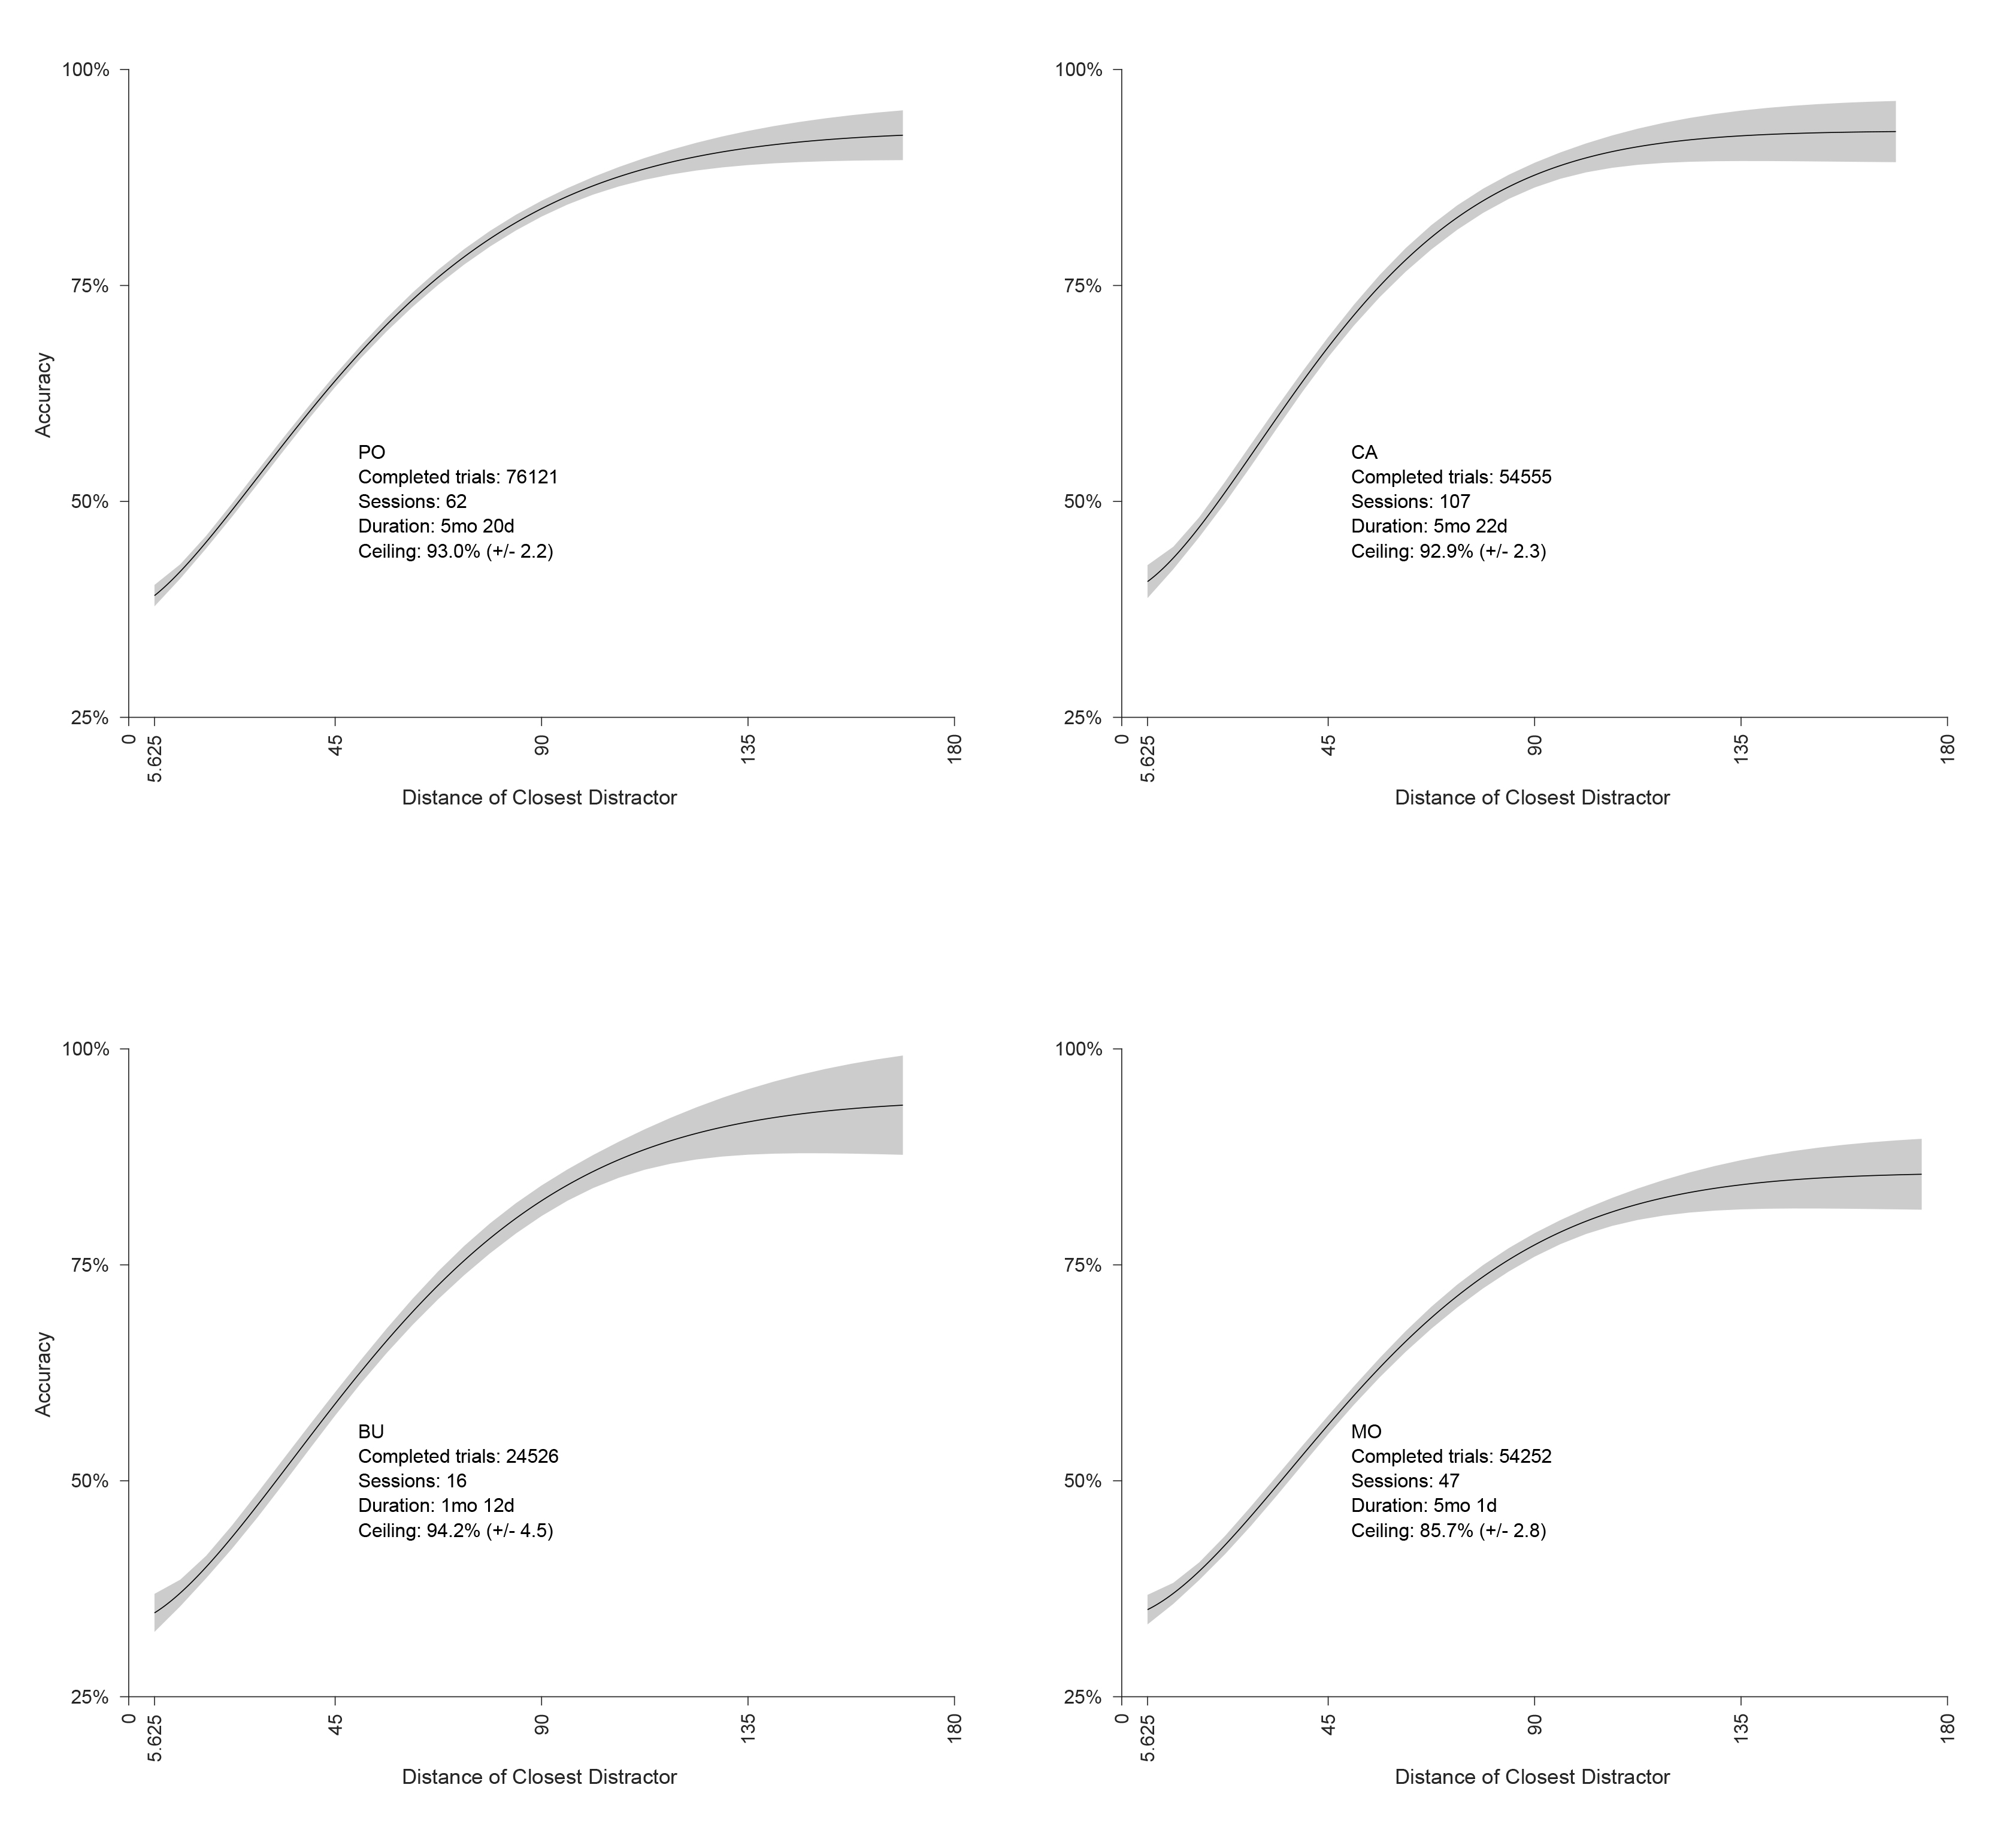
\includegraphics[width=\textwidth+4cm]{Outputs/Paper/Figures/flat/SI1_psychometric.jpg}
    \caption{\textbf{Psychometric functions for the four individual animals (PO, CA, BU, MO) on the color-matching task illustrated in Figure 1.}
    Completed trials for the four animals were: 76121; 54555; 24526; 54252.
    } 
    \label{fig:IndiDiff}
    \end{fullwidth}
\end{figure}

\begin{figure}
    \centering
    \begin{fullwidth}
    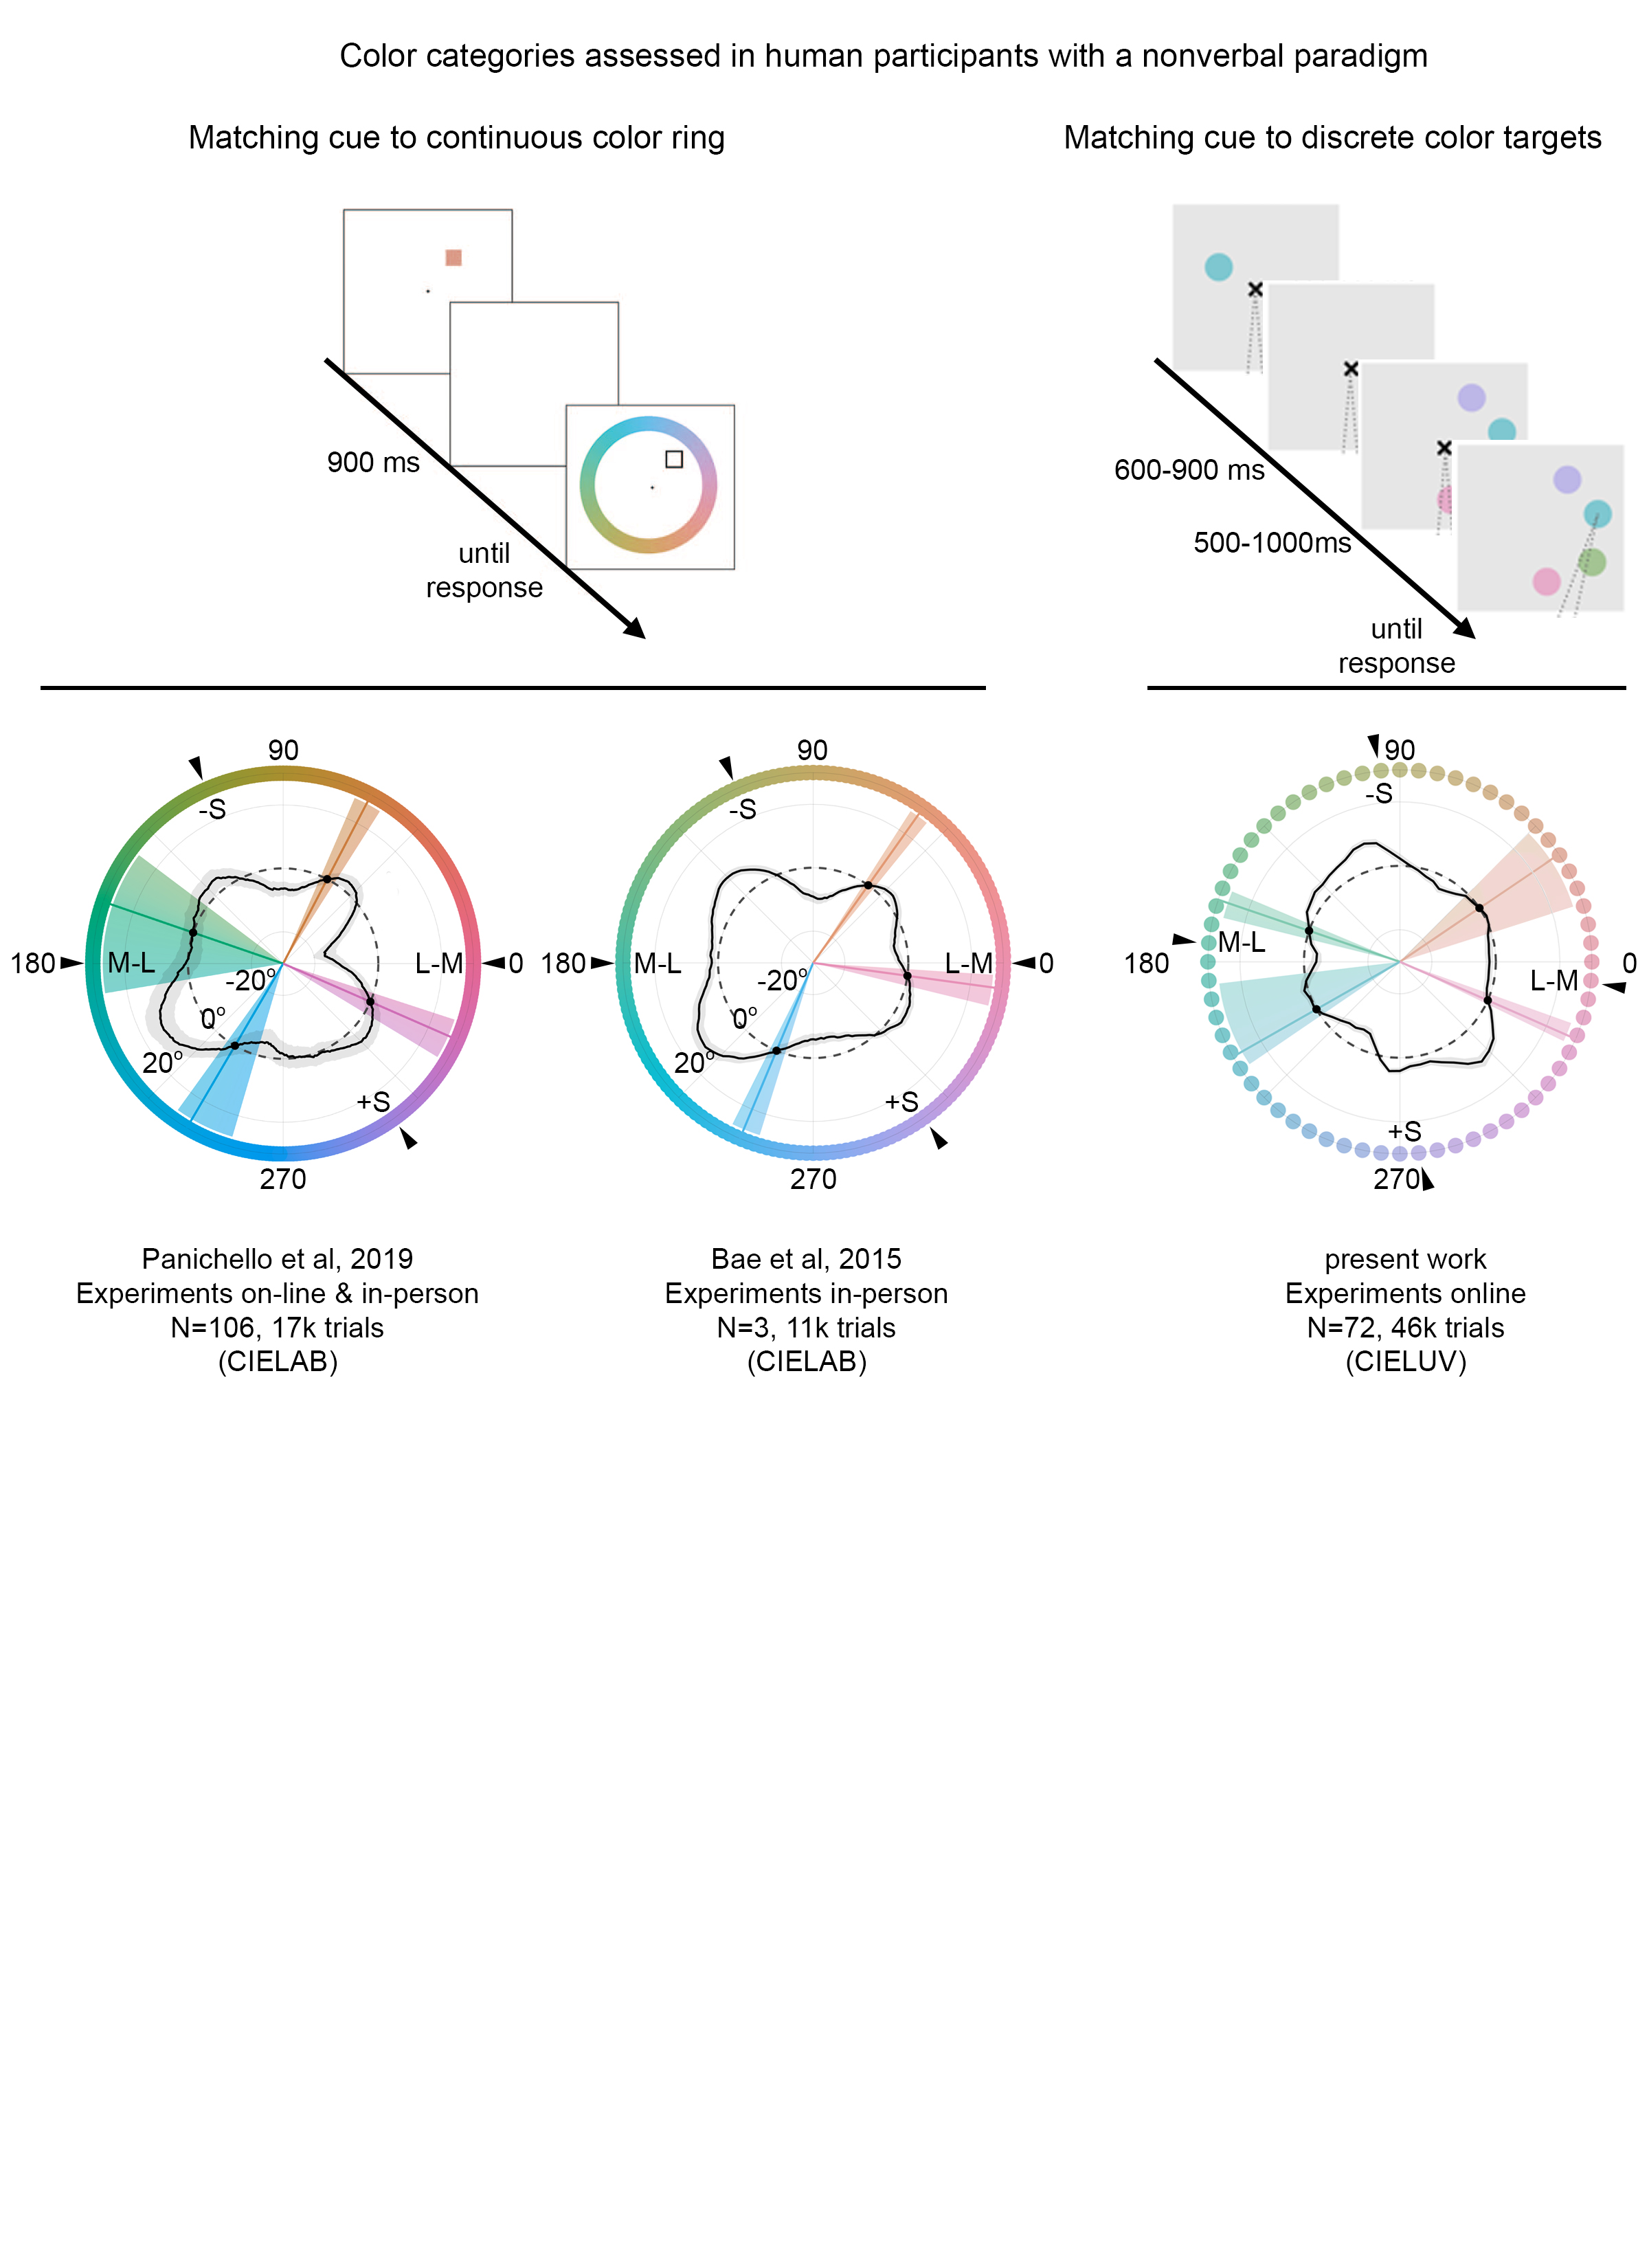
\includegraphics[width=\textwidth+4cm,trim={0 11cm 0 0},clip]{Outputs/Paper/Figures/flat/SI_Human_2.jpg}
    \caption{\textbf{Color categories assessed in human participants with a nonverbal paradigm. }
    Prior work by \citet{bae_why_2015} and \citet{panichello_error-correcting_2019} has used a task in which participants match the color of a cue to a continuous ring of colors; those published results were obtained with a combination of in-person experiments and on-line experiment, with a memory delay and without. The results are broadly consistent, recovering four color categories by mixture-model analysis, corresponding to blue, green, orange and pink. 
    Note that the data from \citep{bae_why_2015} shown in the figure were from just three participants, engaged in a task that had a memory delay; those authors confirmed the results in more subjects with a version of the task that omitted the memory delay period (the cue and the match-option color wheel were presented simultaneously). The present work adapted the paradigm so that the match options in each trial were four discrete targets randomly drawn from 64 colors sampling the color space. The data shown in this figure were obtained in human participants, with experiments conducted online with Amazon Mechanical Turk. These results are again broadly consistent with the prior work using the continuous-matching ring in recovering, by mixture analysis, four significant categories corresponding to blue, green, orange, and pink. We note that the discrete-matching task recovers a trend for a fifth category that would correspond to "purple"; close inspection of the results in \citep{bae_why_2015, panichello_error-correcting_2019} and in studies of human infants \citep{skelton_biological_2017} also show evidence of this trend. The stimuli in the \citep{bae_why_2015, panichello_error-correcting_2019} were defined in CIELAB, while the stimuli in the present work were defined in CIELUV; this difference in color space is associated with a slight clockwise rotation of the cone-opponent axes. The S axis poles provide a useful landmark; they are associated with positive slopes in all three data sets.
    } 
    \label{fig:Human}
    \end{fullwidth}
\end{figure}

\begin{figure}
    \centering
    \begin{fullwidth}
    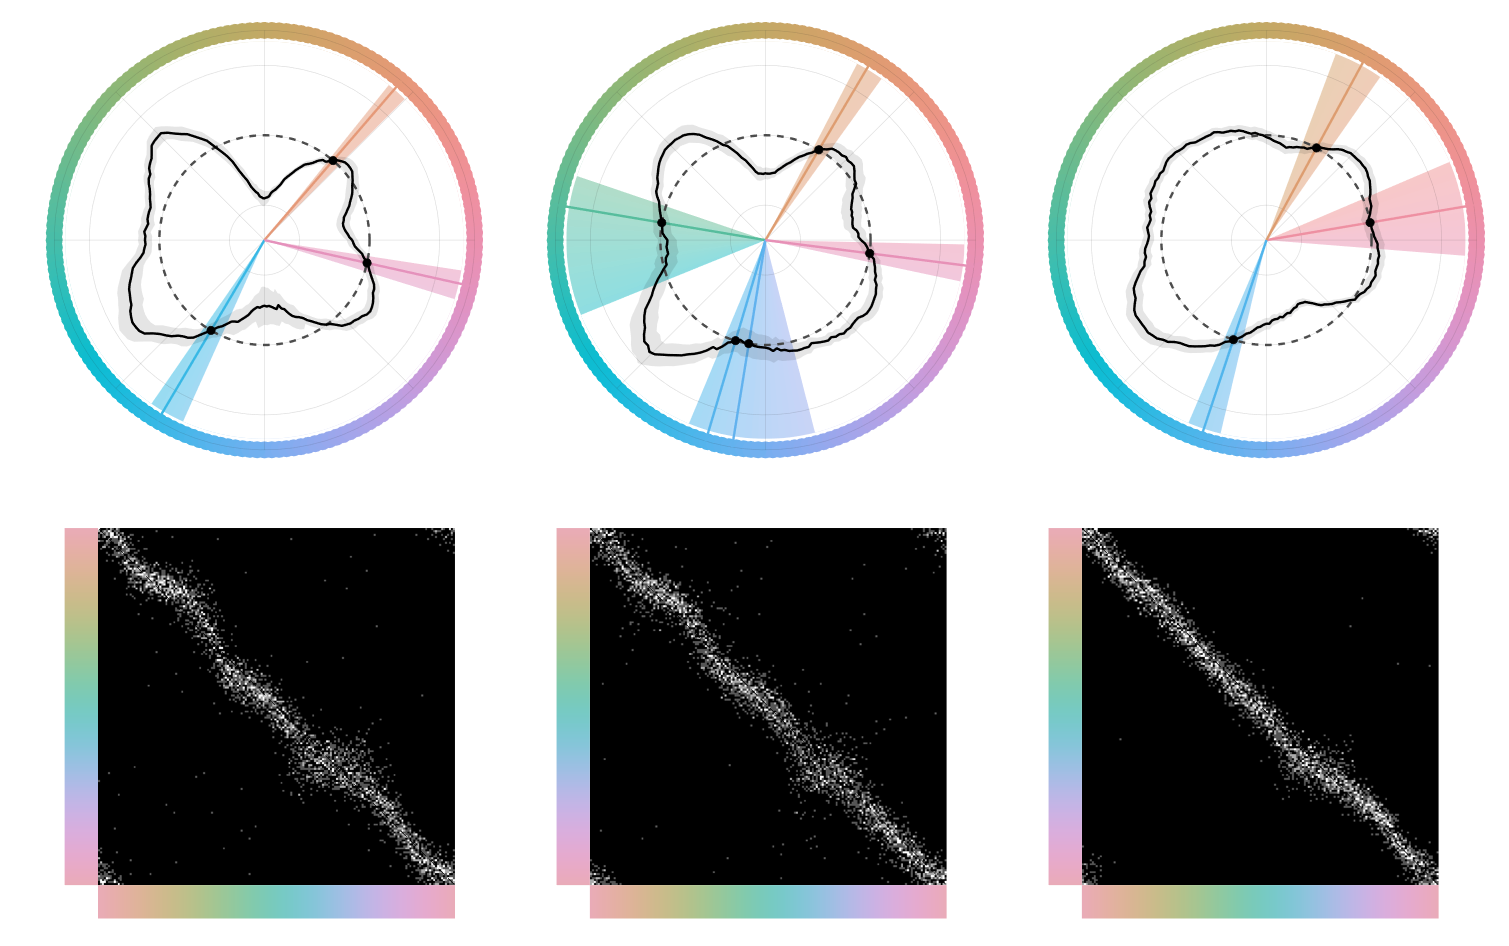
\includegraphics[width=\textwidth+4cm]{Outputs/Paper/Figures/flat/SI_Bae_indi.png}
    \caption{\textbf{Models fit to the individual data of \citet{bae_why_2015} (delayed).}
    The delayed data of \citep{bae_why_2015} consists of data from 3 participants, who completed 3600 trials each, providing sufficient data for a meaningful individual-level analysis.
    We present individual-level mixture models and choice probability matrices.
    The third observer (right) appears to have somewhat diminished cognitive biases compared to the other observers.
    Prior work (such as \citep{bae_why_2015}) has focused on the analysis of aggregated data, partly because this suits the hypotheses they (and we) have sought to test, but also due to technical limitations - using current methods a large amount of data is required, and collecting smaller amounts of data from individuals and then combining it is often a more palatable solution than collecting vast amounts of data from individuals.
    Future work which considers individual differences will be valuable, in part because it is an open question how consensus terms are created within a culture. For example, cognitive biases might only emerge at the group level as a combination of the biases of many individuals, in the same way that a rich representation of color categories is evident in a distributed fashion across human populations that appear to have relatively low informative color-naming systems \citep{lindsey_hunter-gatherer_2015,gibson_color_2017}.
    } 
    \label{fig:Bae_indi}
    \end{fullwidth}
\end{figure}

\begin{figure}
    \centering
    \begin{fullwidth}
    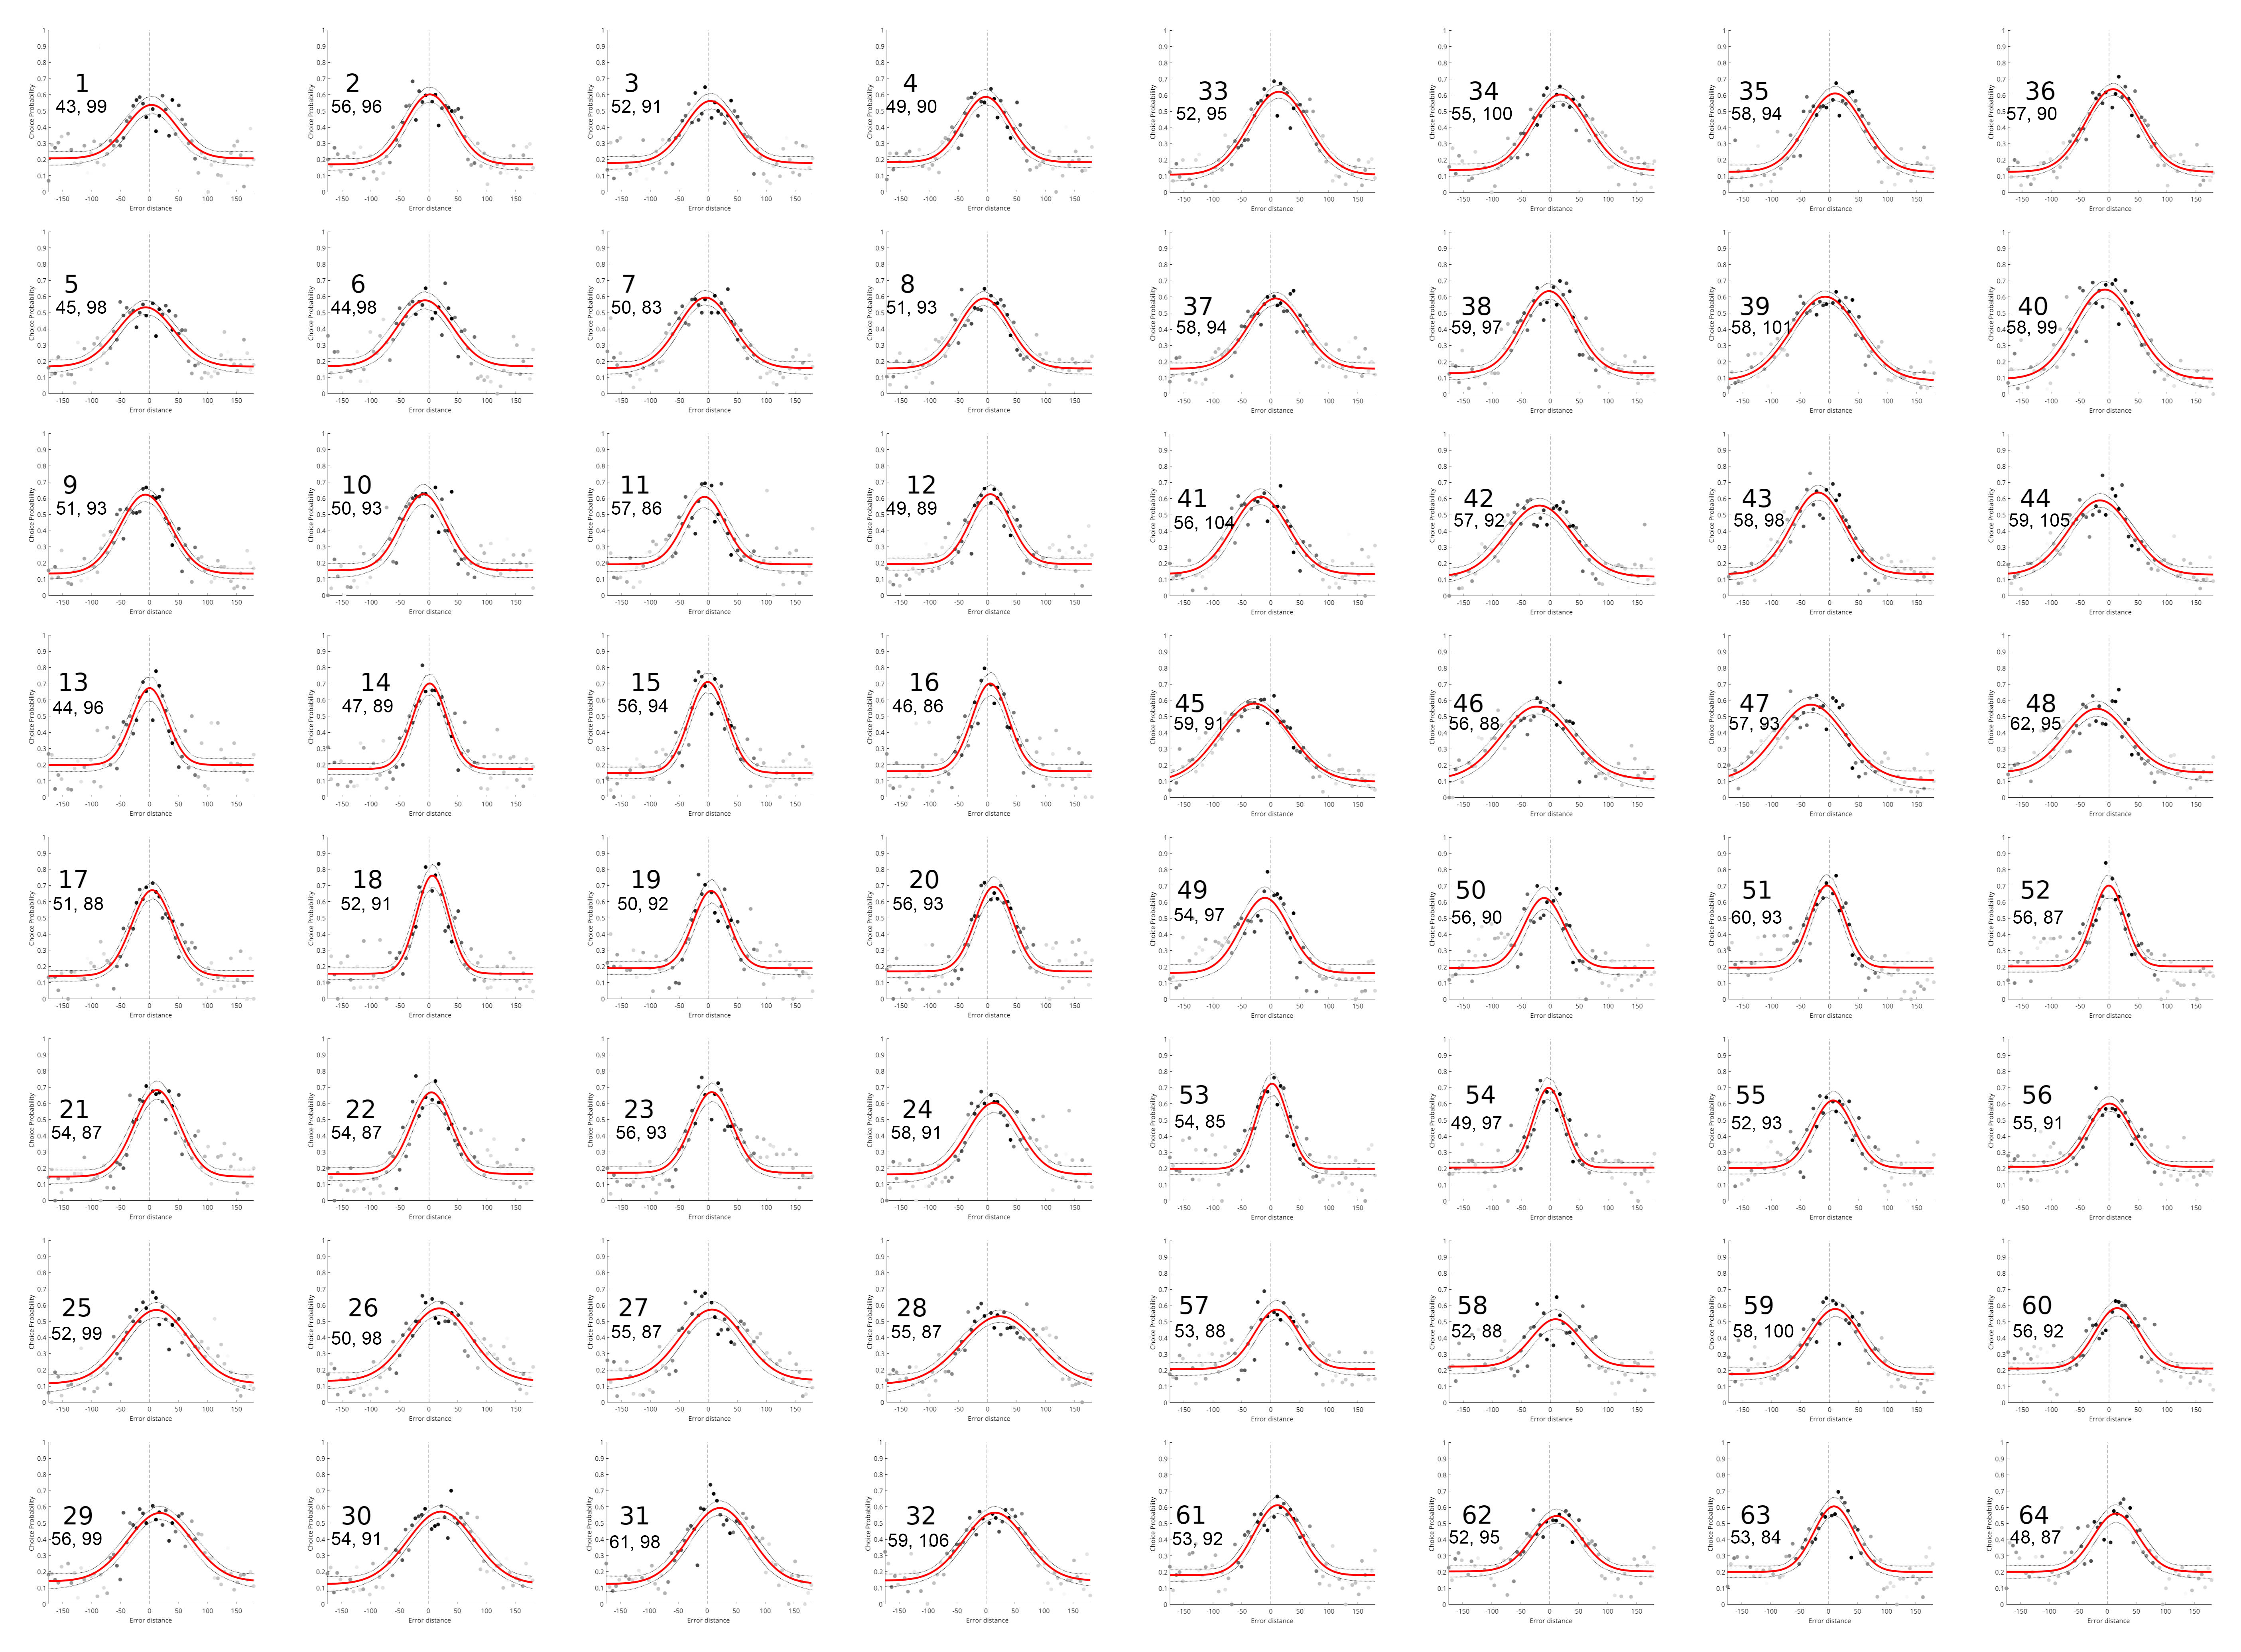
\includegraphics[width=\textwidth+4cm]{Outputs/Paper/Figures/flat/SI3_MMBreakOut_2.jpg}
    \caption{\textbf{Gaussian fits from the Mixture Model.}
    Each trace shows the Gaussian fit for one of the 64 target colors (large number in each panel corresponds to the cue color) used in the color-matching task, as per Equation 1; data averaged over four animals. The extent to which each data point is black versus white indicates the number of trials that provided that choice option, normalized for each cue (the pair of smaller numbers below the cue-color number provides the range: the larger number corresponds to the black symbol, and the smaller number to white); see Methods for how the curves were fit to the data. 
    } 
    \label{fig:MMBreakOut}
    \end{fullwidth}
\end{figure}

\begin{figure}
    \centering
    \begin{fullwidth}
    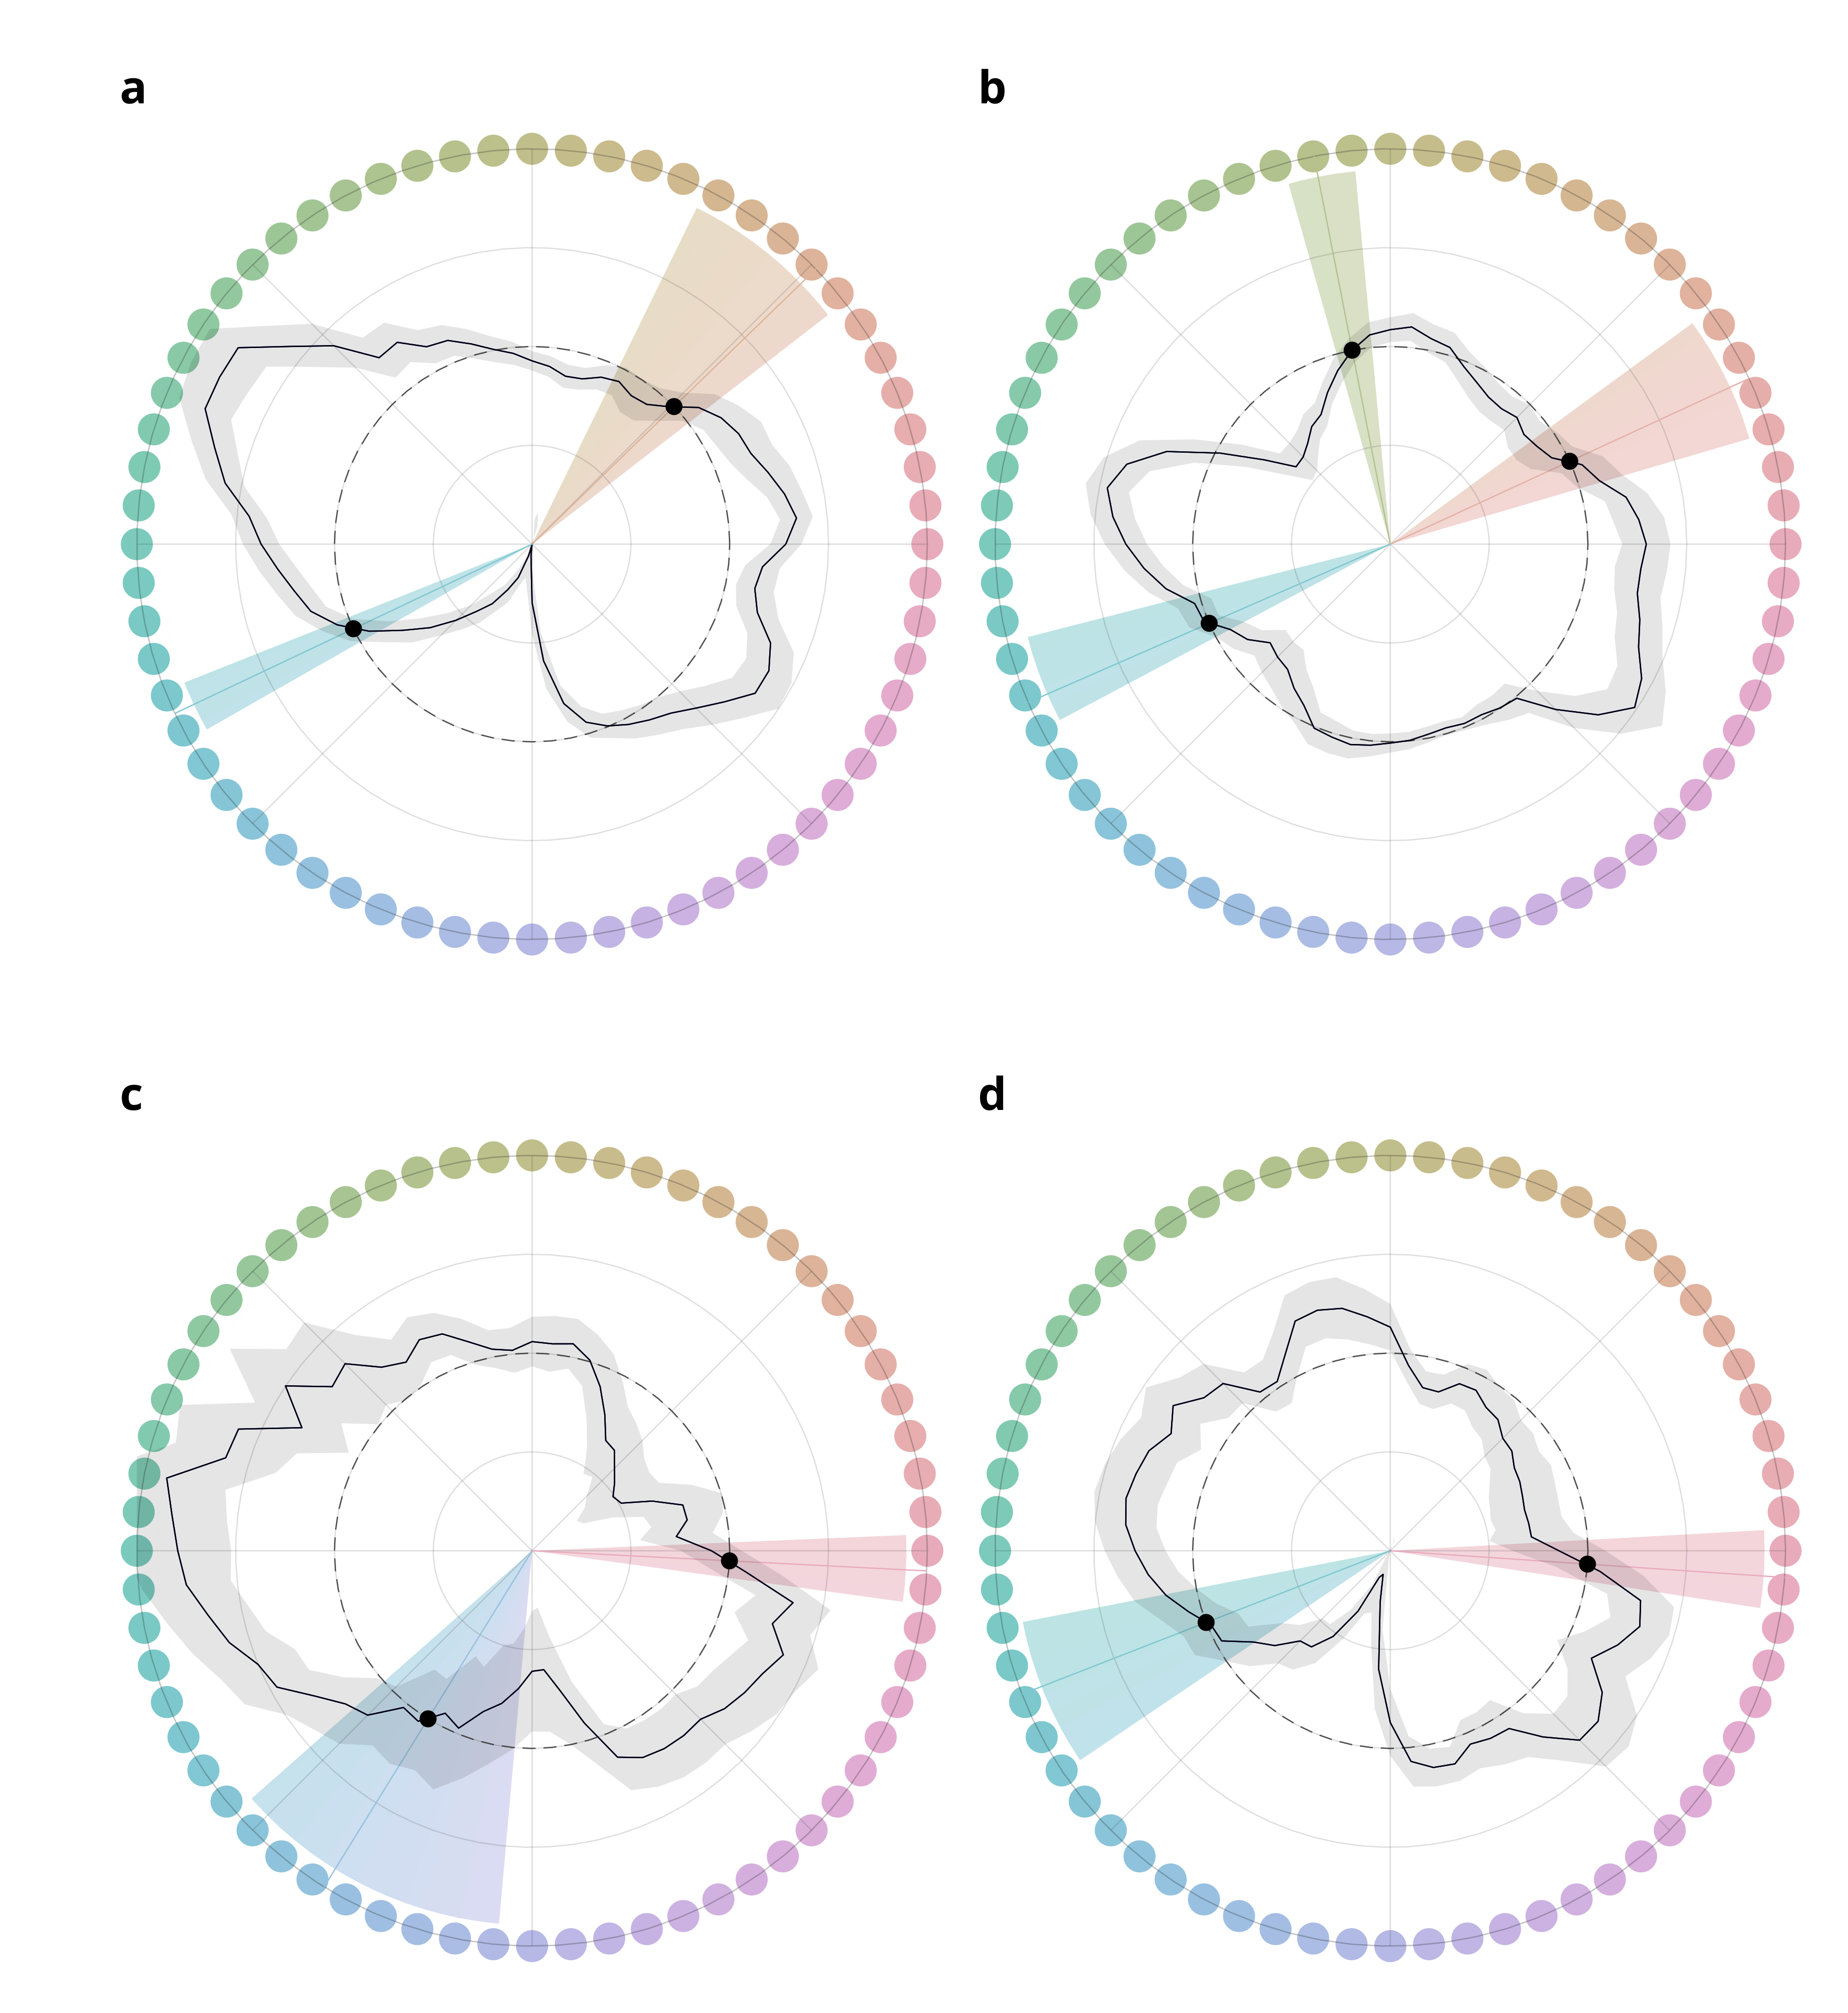
\includegraphics[width=\textwidth+4cm]{Outputs/Paper/Figures/flat/SI4_MM.jpg}
    \caption{\textbf{Mixture-model analysis of the individual data for the four animals in the color-matching task.}
    Data shown in the same format as Figure 2c.
    All data for each animal is included (in contrast to Figures 2bc where data were subsampled to ensure equal contributions from each animal).
    } 
    \label{fig:IndiMM}
    \end{fullwidth}
\end{figure}

\begin{figure}
    \centering
    \begin{fullwidth}
    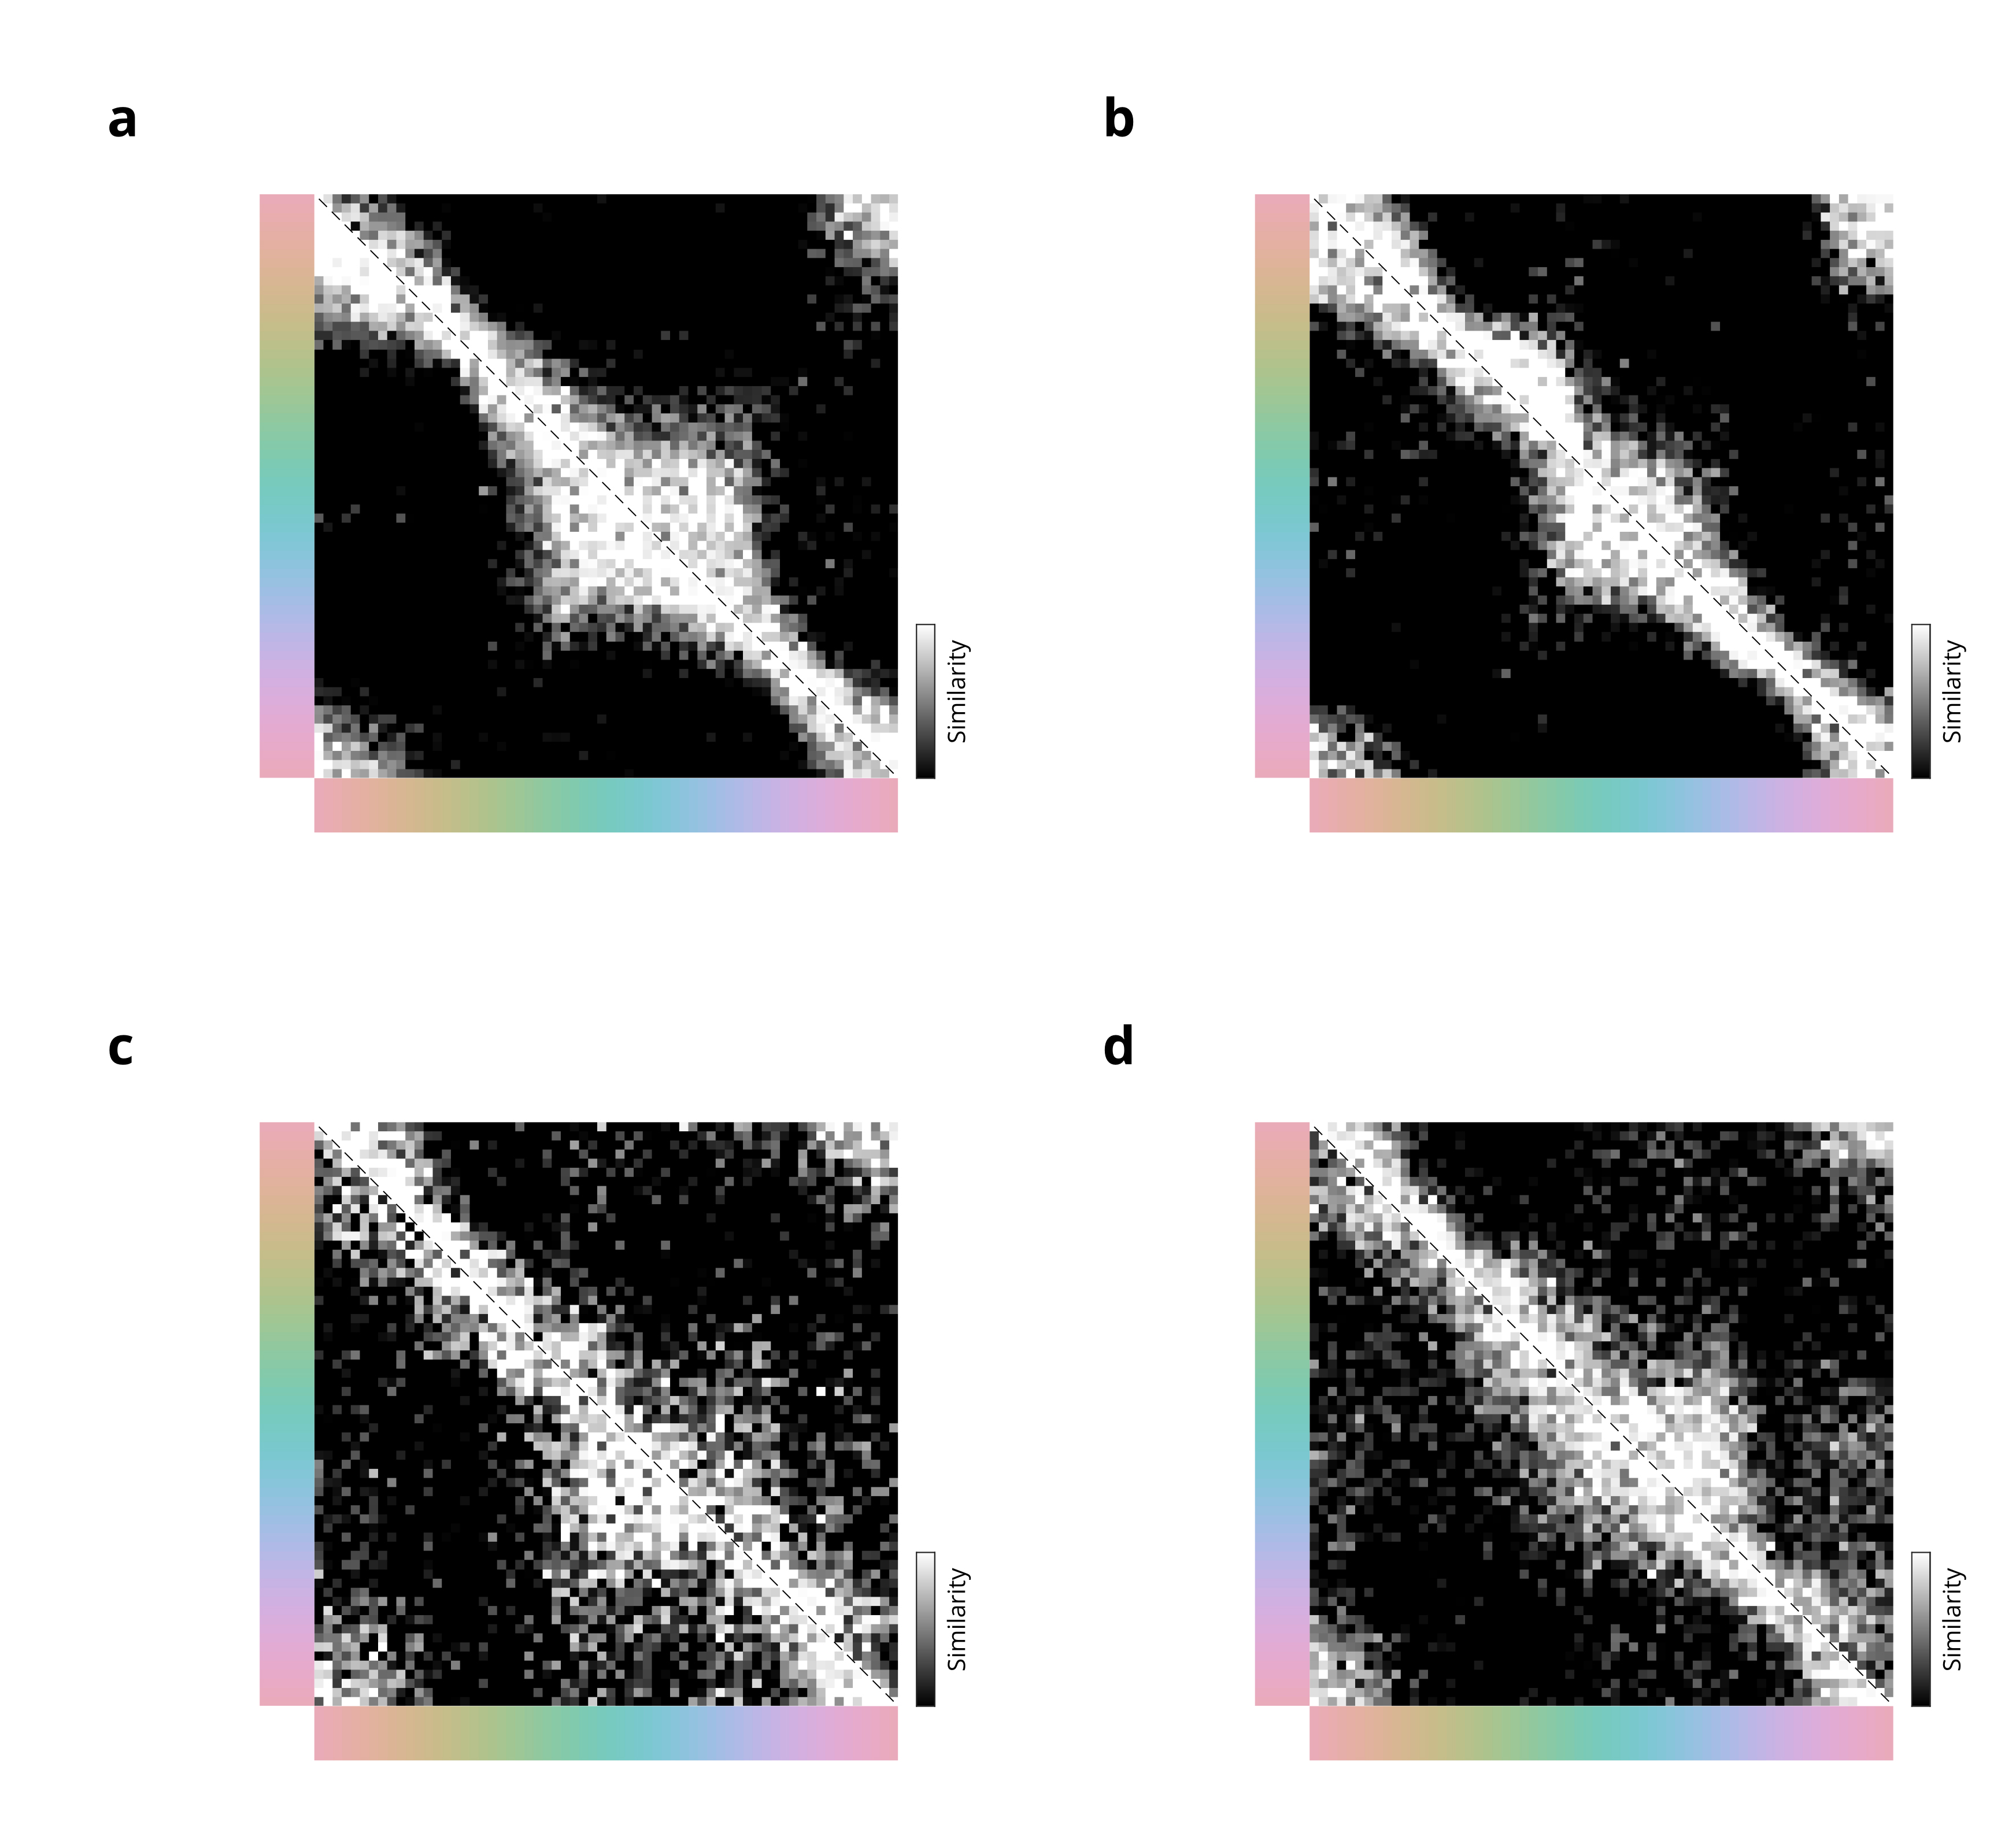
\includegraphics[width=\textwidth+4cm]{Outputs/Paper/Figures/flat/SI5_IndTCCv.jpg}
    \caption{\textbf{Similarity matrices for free similarity matrix models, fit to individual data.}
    The order of the plots is the same as the order in other figures, PO, CA, BU, MO. 
    These plots use the full set of data for each animal.
    See Figure 3ab for data averaged across animals, with data subsampled to ensure the same amount of data per animal.
    } 
    \label{fig:IndiTCC}
    \end{fullwidth}
\end{figure}

\begin{figure}
    \centering
    \begin{fullwidth}
    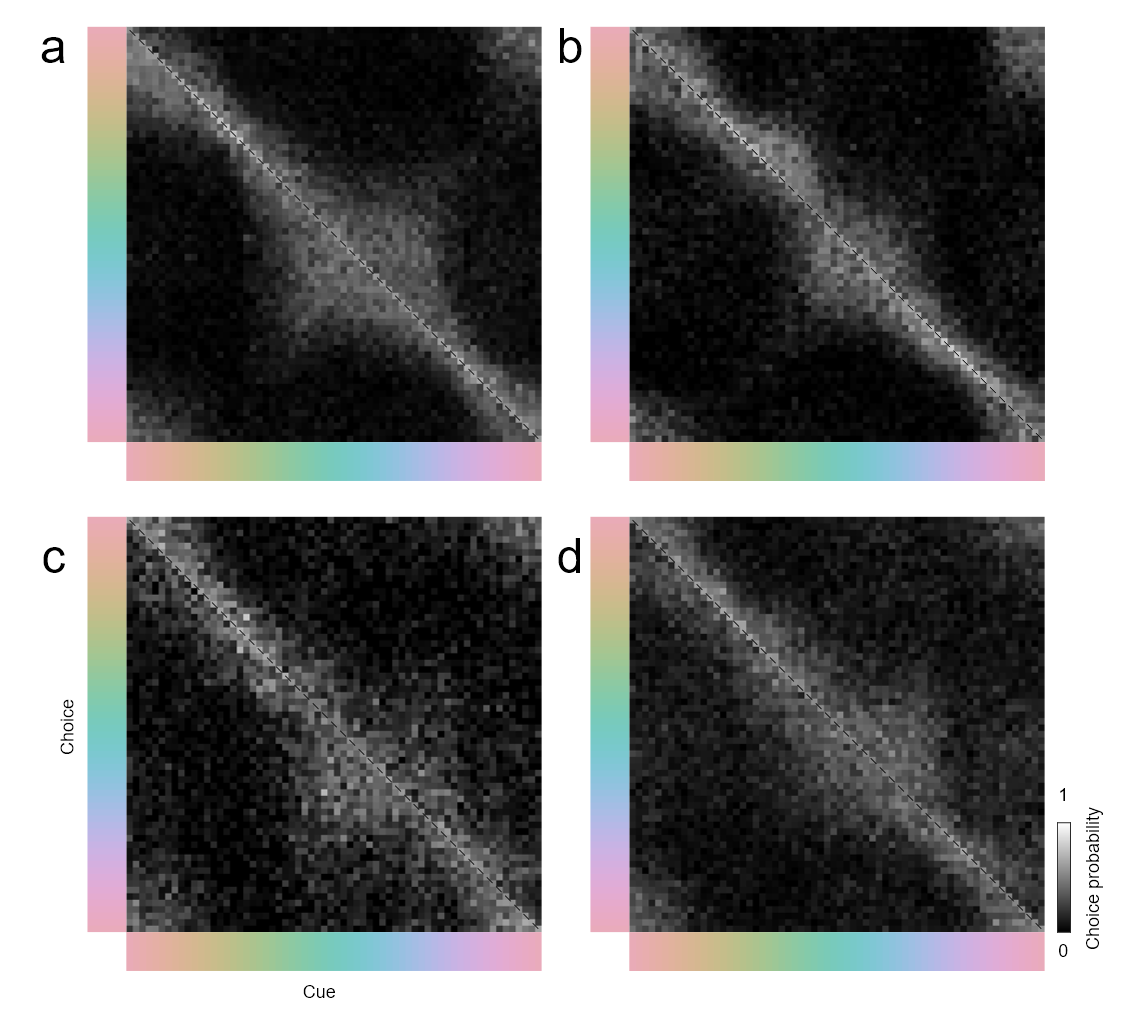
\includegraphics[width=\textwidth+4cm]{Outputs/Paper/Figures/flat/SI6_choiceMatrices.png}
    \caption{\textbf{Choice probability matrices for free similarity matrix models, for the four individuals.}
    As per the similarity matrices presented, each column represents a cue, and each row represents a choice. 
    Here, however, rather than the similarity between cue/choice pairs we show the probability of selection. 
    Whereas the similarity matrix is the output of model fitting, this matrix is derived more directly from the data: each cell is simply the number of times a particular choice was made divided by the number of times that choice was an option. 
    The identity line, representing correct options, appears artificially inflated (see Methods for further information).
    } 
    \label{fig:choiceProbabilityMatrices}
    \end{fullwidth}
\end{figure}

\begin{figure}
    \centering
    \begin{fullwidth}
    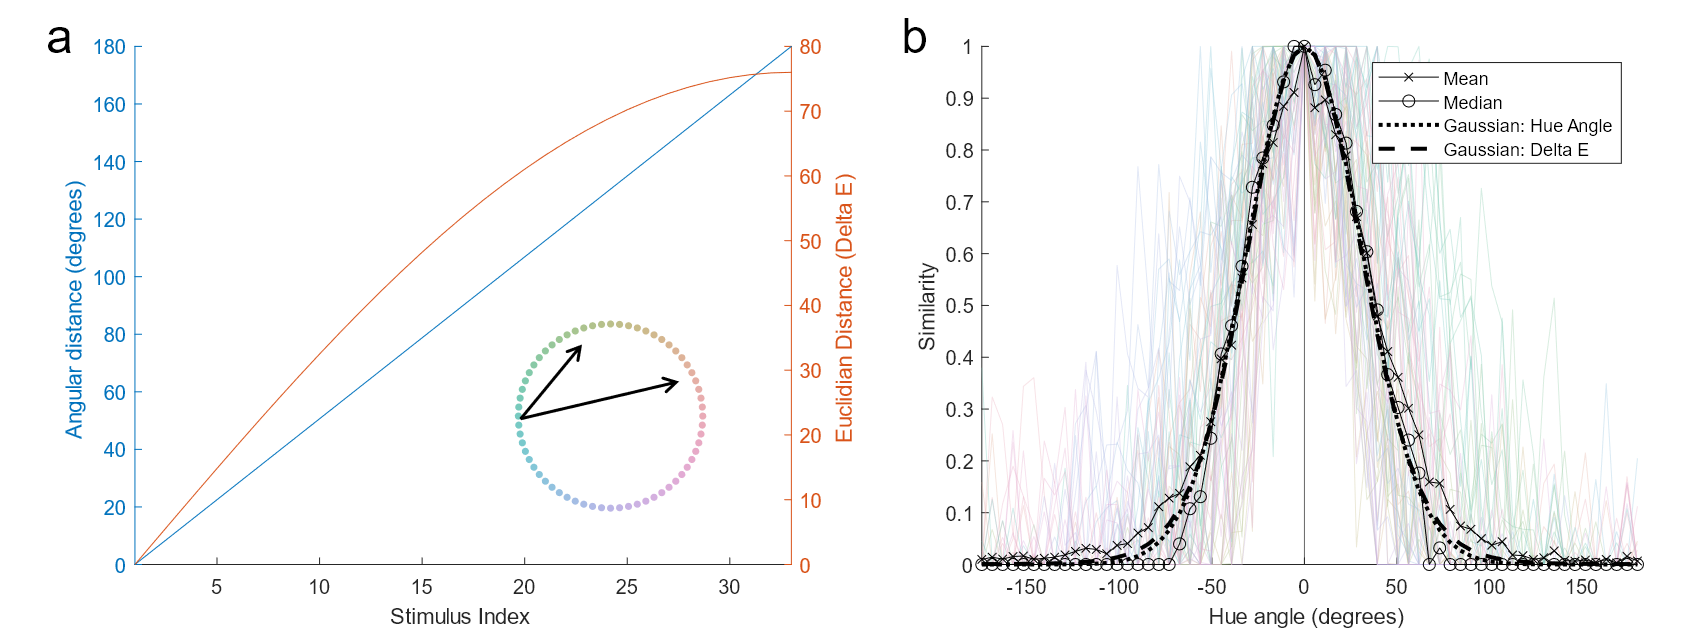
\includegraphics[width=\textwidth+4cm]{Outputs/Paper/Figures/flat/SI7_distanceMetricComparison.png}
    \caption{\textbf{Comparing distance metrics: angular distance vs Euclidean distance.}
    We inherit the practice of using angular distance as our distance metric from prior work \citep{bae_why_2015,panichello_error-correcting_2019}, but another reasonable distance metric exists: the Euclidean distance in CIELAB and CIELUV is referred to as "Delta E". 
	These two metrics are closely correlated at lower values, diverging increasingly at higher values. 
	Using either in our model makes negligible difference, and so in this paper we choose to use angular distance. 
	However, if one were to use a TCC-v model to analyse multi-dimensional data (as opposed to our one-dimensional ring of stimuli) Delta E it seems reasonable that a switch to Delta E would be a sensible path.
	\textbf{a}, Angular distance (hue angle difference) and cartesian distance (Delta E) as a function of stimulus index difference. 
	\textbf{b}, Gaussian fits parameterized by each distance metric. 
	Translucent colored lines are the columns from F4a/b, colored by cue. 
	Dotted and dashed lines are Gaussian fits where the Gaussian is computed as a function of hue angle and Delta E respectively. 
	Note how they diverge, but only slightly, and that both align well with the mean and the mode.
    } 
    \label{fig:distanceMetricComparison}
    \end{fullwidth}
\end{figure}








%%%%%%%%%%%%%%%%%%%%%%%%%%%%%%%%%%%%%%%%%%%%%%%%%%%%%%%%%%%%
%%% ARTICLE END
%%%%%%%%%%%%%%%%%%%%%%%%%%%%%%%%%%%%%%%%%%%%%%%%%%%%%%%%%%%%

\end{document}




